\documentclass[final, a4paper,masters,en,listoffigures,listoftables,norwegiandates]{NMBU}
% Limitation: at this stage, the template is designed only for a4 size paper.

% If you'd like to use chapters instead of sections, add 'book' to the options, as \documentclass[book,...]{NMBU}. Recall that you now have to use \chapter{} and then \section{}, \subsection{}, ... 

\usepackage[nohyperlinks]{acronym} % If you need a List of Acronyms, consider using this package

%\documentclass[final,...]{NMBU} % use "final" when you are done with your thesis (with XeLaTeX)! 

% \usepackage[font=small]{caption} % if you prefer smaller captions
% \captionsetup{width=0.9\linewidth} 

% The NMBU style package is designed to help you write the cover and back page automatically. Make sure to include the information below to generate your title. You can set the language you are writing in with "en" for english, "bm" for bokmål, or "nn" for nynorsk.

% A table of contents is automatically included. If you have more than one figure, you need a list of figures by adding "listoffigures" to the documentclass parameters. If you have more than one table, you need a list of tables by adding "listoftables" to the documentclass parameters.

% If you would like to have a bibliography with named authors, organised alphabetically, add "namedauthors" to the parameters of the document class.
\usepackage{comment}
\usepackage{minted}
\usepackage{xcolor}
\usepackage[utf8]{inputenc}
\usepackage{newunicodechar}
\usepackage{tikz}
\newunicodechar{─}{\textemdash}

\setminted{
  linenos,
  frame=lines,
  fontsize=\small
}


\addbibresource{bib.bib} % here you include the bibliography file. 

% If you are using Norwegian dates in your bibliography, add "norwegiandates" to the document class.

% When you finish your thesis, you can activate the "final" parameter in the document class and switch the LaTeX compiler from pdfLaTeX to XelaTeX (on Overleaf, "Menu"->"Compiler"). This is for 2 reasons: 1) to produce your front page with the Arial font; 2) XeLaTeX produces better fonts and (usually) smaller PDFs. Every kilobyte of space we save helps reduce CO2 emissions :)

% Good luck with your thesis! If you get in trouble with LaTeX stuff, write to me: leonardo.rydin@gmail.com

% In your .tex file, you need to include the following information to produce the first page of your thesis

\title{Investigating the Impact of Axon Activity on Measured Brain Potentials}
\author{Ole Josef Pinaas}
\thesisyear{2025}
\credits{30}
\faculty{Faculty of Science and Technology}
\supervisor{Torbjørn Vefferstad Ness and Gaute Tomas Einevoll} % Include the name of the supervisor or supervisors (this is added to the metadata of the PDF)
%\engtitle{} % Only if you write a thesis in a Scandinavian language

% You should also use the "\abstract" and "\sammendrag" to produce those. If you are writing in a Scandinavian language, the sammendrag will appear first.

\abstract{
This thesis investigates the impact of axonal activity on measured brain potentials, emphasizing the biophysical mechanisms underlying electroencephalography (EEG) and electrocorticography (ECoG) signals. Through computational modeling and simulation using detailed neuron models in the NEURON simulation environment and extracellular potential computations with LFPy, the study explores how action potentials (APs) generated in axons contribute to extracellular potentials. Specifically, the influence of axonal signals on the amplitude and waveform of recorded extracellular potentials was systematically examined across varying neuron populations and electrode configurations. Results indicate that axonal activities can affect both the shape and amplitude of measured signals, especially under conditions resembling experimental EEG and ECoG recordings, for synchronized and large populations. The study highlights important implications for interpreting electrophysiological data, particularly regarding source localization and the biophysical basis underlying brain imaging techniques. Additionally, limitations such as the idealized modeling assumptions and recommendations for future research are discussed.
}

\sammendrag{
Denne masteroppgaven undersøker hvordan aksonal aktivitet påvirker målte hjernepotensialer, med særlig vekt på biofysiske mekanismer bak signaler fra elektroencefalografi (EEG) og elektrokortikografi (ECoG). Gjennom datamodellering og simulering med detaljerte nevronmodeller i NEURON-simuleringsmiljøet, samt beregning av ekstracellulære potensialer med verktøyet LFPy, utforskes det hvordan aksjonspotensialer (AP) generert i aksoner bidrar til ekstracellulære potensialer. Spesielt undersøkes systematisk hvordan aksjonspotensialer påvirker amplituden og bølgeformen til registrerte ekstracellulære potensialer for ulike nevronpopulasjoner og elektrodeoppsett. Resultatene indikerer at aksonal aktivitet kan påvirke både form og amplitude av målte signaler, spesielt under forhold som ligner eksperimentelle EEG- og ECoG-målinger med store og synkroniserte populasjoner. Studien belyser viktige implikasjoner for tolkning av elektrofysiologiske data, særlig med hensyn til kildelokalisering og det biofysiske grunnlaget for hjerneavbildningsteknikker. I tillegg diskuteres begrensninger knyttet til idealiserte modelleringsforutsetninger, samt anbefalinger for fremtidig forskning.
}


\acknowledgements{
This thesis marks the end of my (first) 5 years at the Norwegian University of Life Sciences. It is the culmination of many nights and some days spent studying chiefly at home, but also in different lectures and study-groups around campus. First I would like to thank my supervisor Dr Torbjørn V. Ness. Things didn't always look very promising, but here we are. Thank you for your great answers, questions, suggestions, and critical comments. I am very grateful for the time you committed (both during and outside of office hours) to guiding me through this project. A special thank you also for my secondary advisor Prof. Gaute T. Einevoll who introduced me to this field with your excellent and enthusiastic teaching of FYS388 - Computational Neuroscience here at NMBU. 
\newline
\newline
I would also like to say thank you to all my fellow students and especially my roommates for both your critical thoughts and great companionship. A special thank you to Richard. Without your "stupid" questions, frequent sanity checks and great feedback this thesis would not be possible. Also, thank you for taking care of me with all the amazing food. :)
\newline
\newline
I also have a lot of gratitude to my family and friends. Without your support, both in the form of proofreading, pity, encouraging words, and sometimes a kind "man up and get it done" this thesis would not have been finished on time. 
\newline
\newline
My biggest thank you goes to you Inga. You have been my light at the end of the tunnel and for that I will be forever grateful.
\begin{flushleft}           
\vspace{1.5cm}             
Ås, \today        
\\[1cm]                    
\makebox[5cm]{\hrulefill}  
\\[0.2cm]                 
\text{Ole Josef Pinaas}  
\end{flushleft}

}


 %You can add acknowledgements here. In Scandinavian languages, use "\foreword{}" (or if in English you prefer Foreword to Acknowledgements). The foreword comes before the abstract.

\begin{document}

\section*{List of Acronyms}
\begin{acronym}
    \acro{AI}{Artificial Intelligence}
    \acro{AP}{Action Potential}
    \acro{CSF}{CerebroSpinal Fluid}
    \acro{ECoG}{ElectroCorticoGraphy}
    \acro{EEG}{ElectroEncephaloGraphy}
    \acro{EPSP}{Excitatory PostSynaptic Potential}
    \acro{ERP}{Event Related Potential}
    \acro{fMRI}{functional Magnetic Resonance Imaging}
    \acro{IPSP}{Inhibitory PostSynaptic Potential}
    \acro{LFP}{Local Field Potential}
    \acro{MEG}{MagnetoEncephaloGraphy}
    \acro{PET}{Positron Emission Tomography}
    \acro{PSP}{PostSynaptic Potential}
\end{acronym}

\startthesis % This command will separate the Roman-numbered pages above and the Arabic-numbered pages below as well as create the table of contents, list of figures, and list of tables.


\section{Introduction} \label{sec: introduction}
Since the dawn of consciousness, humans have tried to understand others and themselves. What makes us human is a question best left to philosophers, but understanding the physical mechanics of the brain is an enigma that scientists have been unraveling for centuries \cite{finger1994origins}. Although the field has advanced a lot since we first started exploring the human brain, there are still more questions than answers.

The importance of the brain was first known as far back as Ancient Egypt, when it was described by scholars of the 17th century BC in the \textit{Edwin Smith Papyrus}. This medical text focused on the scientific side of medicine which, at the time, was usually rooted in the belief in magic. It detailed several neurological symptoms such as dysphasia and seizures, as well as describing the surface of the brain and the surrounding tissues \cite{kandel2021principles}. Further theories on brain function were incorporated in \textit{The Hippocratic Corpus} based on the teachings of Hippocrates, who is widely regarded as the father of western medicine \cite{Hippocratesinfluenceontheoriginsofneurosurgery, Koutserimpas2024hippocrates}. The document references the divided structure of the cerebrum, conventionally recognized as the brain, as well as describing the meninges, a layer of protective membranes around the brain and brainstem \cite{breitenfeld2014hippocrates}. In reality the brain is composed of many different parts. The most basic division is outlined in Figure \ref{fig:Brainparts} and includes the two halves of the cerebrum, as well as the brain stem, and the cerebellum \cite{Swanson2000}.

\begin{figure}[h]
    \centering
    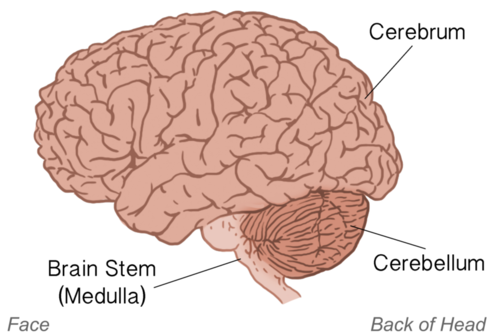
\includegraphics[width=0.5\linewidth]{Figures/3_major_parts_of_the_brain.png}
    \caption{The three major parts of the human brain: cerebrum, cerebellum, and brain stem. Image by Laura Guerin / CK-12 Foundation, licensed under \href{https://creativecommons.org/licenses/by-sa/3.0/}{CC BY-SA 3.0}. Source: \href{https://commons.wikimedia.org/wiki/File:3_major_parts_of_the_brain.png}{Wikimedia Commons}.}
    \label{fig:Brainparts}
\end{figure}

Neural signals are fundamentally electrical, a concept first demonstrated in the 18th century by Luigi Galvani through experiments on muscle contractions in frogs \cite{PICCOLINO1998AnimalElectricity}. Modern neuroscience has since confirmed that neurons communicate via rapid electrical impulses called action potentials. These arise from ion flows across the cell membrane, primarily involving sodium and potassium ions moving through voltage-gated channels \cite{hodgkin1952quantitative}. The neuron's membrane behaves like a circuit element, enabling voltage changes that allow signals to travel along axons. In addition to these fast spikes, slower electrical fluctuations occur in dendrites during synaptic activity, contributing to the brain's overall extracellular electric field \cite{Halnes2024ElectricBrainSignals}.

The realization that these electrical signals could be detected from outside the skull marked a turning point in neuroscience. In 1924, German psychiatrist Hans Berger made the first successful recording of the brain’s electrical activity from the human scalp. Using a string galvanometer and electrodes made from silver wires, he observed rhythmic voltage fluctuations that reflected ongoing brain processes. Most notably, what he called the alpha rhythm \cite{berger1929elektroenkephalogramm}. Berger’s work provided the first direct evidence that the brain’s electrical activity was not only measurable but also patterned and meaningful. Although initially met with skepticism, his findings were soon replicated, establishing electroencephalography (EEG) as a revolutionary tool in brain research \cite{Halnes2024ElectricBrainSignals, finger1994origins, kandel2021principles}. 

Following Berger’s discovery, EEG technology advanced rapidly in both methodology and application. Key discoveries and technological breakthroughs in this rapid evolution is outlined in Figure \ref{fig:timeline}. During the mid-20th century, improvements in amplifier design, electrode materials, and signal processing enabled more accurate and widespread use of EEG in clinical and research settings \cite{Friston2009Modalities, Benbadis2020, BIASIUCCI2019R80}. The technique proved particularly valuable in diagnosing neurological conditions such as epilepsy, sleep disorders, and brain injuries \cite{Joshi2021}. By the 1960s and 70s, researchers began using EEG to study cognitive processes, giving rise to event-related potentials (ERPs)—voltage changes time-locked to specific stimuli or tasks. In recent decades, advances in computing and signal analysis have further refined EEG, allowing for sophisticated modeling, source localization, and integration with other neuroimaging methods \cite{MULERT200483, Halnes2024ElectricBrainSignals}. Today, EEG remains a cornerstone of both basic and applied neuroscience due to its high temporal resolution, non-invasiveness, and relative affordability.

\begin{figure}[h]
    \centering
    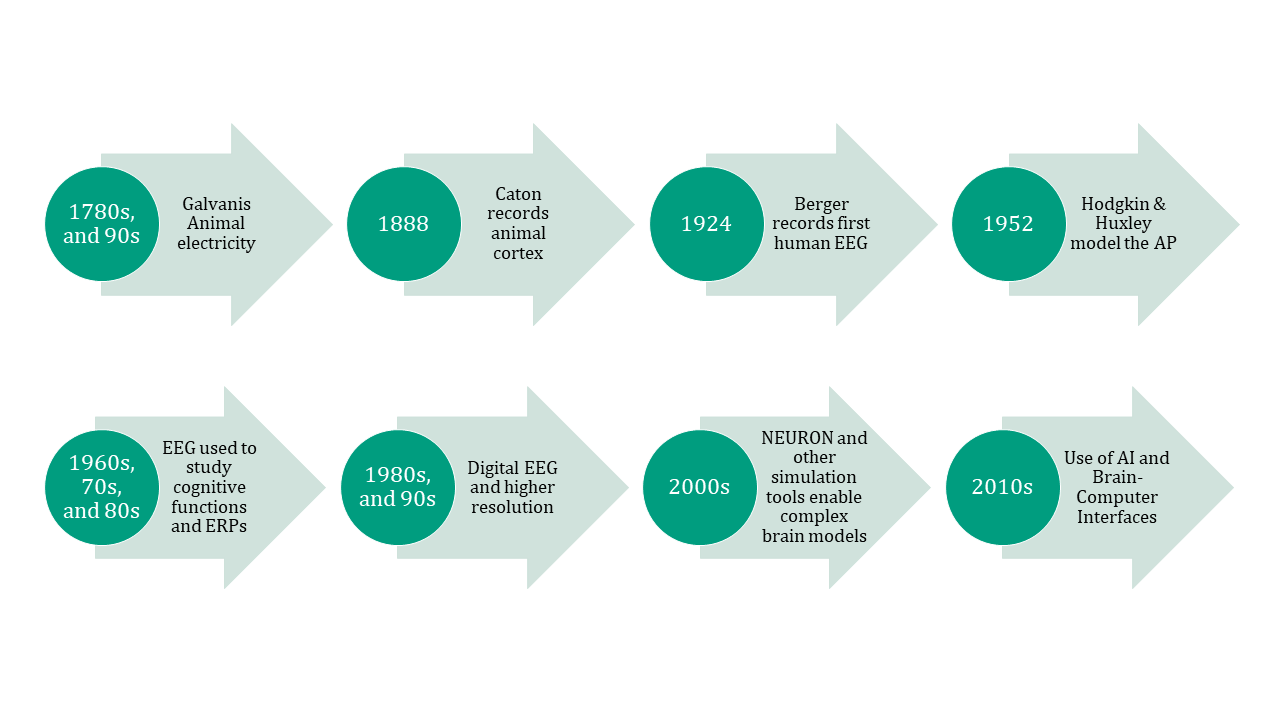
\includegraphics[width=\linewidth]{Figures/TimelineDiscoveries.png}
    \caption{A timeline of important milestones in the field of neuroscience focusing especially on advancements important to this thesis.}
    \label{fig:timeline}
\end{figure}

While EEG is one of the most widely used methods for measuring brain activity, several other modalities offer complementary insights into neural function. Magnetoencephalography (MEG) detects the magnetic fields generated by electrical currents in neurons, providing excellent temporal resolution similar to EEG, but with better spatial precision under certain conditions. Electrocorticography (ECoG) involves placing electrodes directly on the surface of the cortex, typically during neurosurgical procedures, yielding high-resolution recordings with superior signal-to-noise ratios compared to scalp EEG. These modalities are also outlined in Figure \ref{fig:modalities} that illustrates the different placements and measuring locations. Functional magnetic resonance imaging (fMRI), by contrast, measures blood-oxygen-level-dependent (BOLD) signals, offering high spatial resolution but limited temporal precision due to the sluggish nature of hemodynamic responses. Other techniques like positron emission tomography (PET) and intracranial recordings (depth electrodes) further expand the toolbox available for investigating brain function, each with its own trade-offs between invasiveness, resolution, and interpretability \cite{Friston2009Modalities}. Together, these methods provide a multidimensional view of brain activity, with EEG standing out for its unique combination of non-invasiveness, portability, and temporal resolution.


\begin{figure}[h]
    \centering
    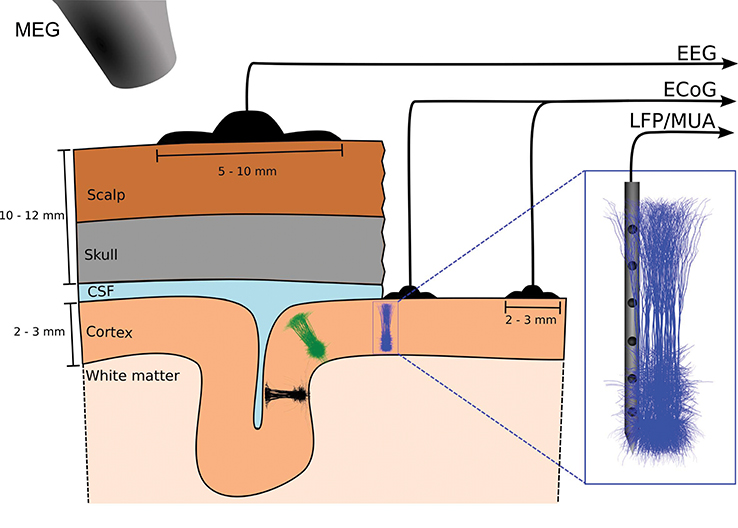
\includegraphics[width=0.7\linewidth]{Figures/modalities.jpg}
    \caption{Illustration of different modalities for measuring brain activity, including magnetoencephalography (MEG), electroencephalography (EEG), electrocorticography (ECoG), and local field potentials/multi-unit activity (LFP/MUA).
    The diagram shows the relative electrode placements and anatomical barriers (scalp, skull, cerebrospinal fluid, cortex, white matter), with approximate distances indicated. MEG sensors measure magnetic fields outside the scalp, EEG electrodes are placed on the scalp, ECoG electrodes rest directly on the cortical surface, and LFP/MUA electrodes penetrate into the brain tissue. The blue, black, and green markings in the cortex illustrate populations of pyramidal cells. 
    \footnotesize Adapted from Hagen et al. \cite{Hagen2018} Licensed under CC BY 4.0.}
    \label{fig:modalities}
\end{figure}



This thesis focuses on the EEG modality as a tool for measuring brain activity, with particular emphasis on the contribution of axons to brain potentials and EEG signals. The central research question is:
\textbf{What contribution do axons have to brain potentials and/or EEG signals?}
To explore this, the project builds on the theoretical framework and methodologies presented in the book Electric Brain Signals by Halnes et al. \cite{Halnes2024ElectricBrainSignals}, which offers a detailed foundation for simulating and interpreting extracellular neural signals. Simulations are conducted using computational models implemented in LFPy, allowing for controlled comparisons between neuronal compartments and population-level effects. The goal is to assess whether axons, often considered negligible in EEG modeling, may in fact have a measurable impact under realistic conditions.

\clearpage
\section{Theory} \label{sec:theory}
This section outlines the required background knowledge required to understand the basics of biophysical modeling of neurons. It also touches upon the current assumptions around forward modeling of brain potentials, both for EEG and for closer field measurements.  
\subsection{Biophysical Models of Neuronal Dynamics} \label{subsec: biophysical models}

Neuronal activity can be described using biophysical models that simulate how voltage signals propagate along the complex morphology of neurons. One of the foundational frameworks in this context is cable theory, which models dendrites and axons as cylindrical cables that transmit electrical signals with both spatial and temporal attenuation. This theory, first proposed to understand dendritic processing, forms the basis for many modern computational models of neuronal dynamics \cite{rall1959branchingdendrites, koch1999BiophysicComputation, Halnes2024ElectricBrainSignals}.

In its one-dimensional form, the cable equation is derived from the principles of current conservation and passive electrical circuit theory. It is expressed as:

\begin{equation} \label{eq: cable equation}
\lambda^2 \frac{\partial^2 V(x,t)}{\partial x^2} = \tau \frac{\partial V(x,t)}{\partial t} + V(x,t),
\end{equation}

where $V(x,t)$ is the membrane potential at position $x$ and time $t$, $\lambda$ is the space (or length) constant, and $\tau$ is the membrane time constant. The equation describes how a voltage disturbance spreads and decays along a cable-like neuronal process.

Biophysical models can be broadly categorized into \textit{passive} and \textit{active} models. Passive models include only linear, ohmic conductances and membrane capacitance. These models are sufficient for describing subthreshold membrane dynamics and are often used in modeling the contributions of dendritic and synaptic currents to extracellular potentials such as local field potentials (LFPs) and electroencephalography (EEG) signals \cite{Halnes2024ElectricBrainSignals}.

Active models incorporate voltage-gated ion channels, which introduce nonlinear dynamics and enable the neuron to generate action potentials. The classical Hodgkin-Huxley model quantitatively describes these active processes, accounting for sodium and potassium currents responsible for the rapid depolarization and repolarization of the membrane during a spike \cite{hodgkin1952quantitative}. Active models are essential for capturing phenomena like backpropagating action potentials, axonal spike propagation, and associated return currents, which can significantly influence extracellular signals under certain conditions.

In modern computational neuroscience, neurons are modeled as multicompartmental systems using simulation tools such as NEURON. Each segment (compartment) of the neuron is treated as a node in an electrical circuit, with its own set of differential equations describing voltage and current dynamics. This approach allows for spatially resolved modeling of transmembrane currents and their contributions to extracellular fields, which is crucial for interpreting EEG and ECoG signals.

Although traditional EEG modeling has emphasized dendritic contributions, recent work suggests that axonal compartments, particularly during synchronous activity or in the presence of myelination, may also play a measurable role in shaping extracellular potentials \cite{ness2016subthreshold, Halnes2024ElectricBrainSignals}. As such, accurate modeling of both passive and active neuronal properties is necessary when assessing the full range of sources contributing to macroscopic brain signals.

\subsection{Structure and Function of Cortical Pyramidal Neurons}

\subsubsection{Basic Neuron Structure} 
Neurons come in a variety of shapes and sizes, commonly classified by their morphology. Examples include star-shaped \textit{stellate cells} and the quintessential \textit{pyramidal cells} of the cortex \cite{Bear2015}. Despite their diversity, most neurons share the same basic anatomical components: a cell body, dendrites, and an axon. The cell body, or \textit{soma}, contains the nucleus and major organelles, similar to other mammalian cells \cite{Nelson2004}. Extending from the soma are the \textit{dendrites} – branching structures that receive input from other neurons. Most neurons have an elaborate dendritic tree that increases the surface area for synaptic contacts. At the opposite end of the neuron, emerging typically from the soma or proximal dendrite, is the \textit{axon}: a long, thin process that carries the neuron's output signal. Axons can extend a considerable distance and often give off branches, allowing one neuron to transmit information to multiple targets \cite{kandel2021principles}. This arrangement of dendrites and axon imparts a functional polarity to the neuron, with dendrites acting as the input region and the axon as the output pathway.

Synaptic connections are formed when the axon terminal of one neuron contacts the dendrite (or soma) of another. Such contacts, called \textit{synapses}, are the primary sites of interneuronal communication. At excitatory synapses onto cortical neurons, the contact is often made onto specialized small protrusions on the dendrites known as \textit{dendritic spines} \cite{Spruston2008}. These spines densely cover the dendrites of pyramidal neurons and serve as discrete postsynaptic compartments for receiving neurotransmitter signals. The morphology of spines (with a bulbous head connected by a narrow neck) is thought to help isolate and modulate synaptic inputs, contributing to synaptic plasticity and computational properties of the neuron \cite{Spruston2008}. Inhibitory synapses, in contrast, commonly target the dendritic shaft or the soma directly. The spatial arrangement of synapses – excitatory inputs mostly on distal dendritic spines and inhibitory inputs often on or near the soma – is important for how signals are integrated by the neuron. Overall, the structural design of neurons, with branched dendrites converging onto a central soma and a single projecting axon, allows them to integrate thousands of incoming signals and convey the processed output to other cells.

\subsubsection{Neuronal Signaling Mechanisms} Neurons are unique in their ability to rapidly propagate electrical signals. This capability arises from the electrical excitability of their cell membrane, which is regulated by ion channels. At rest, a neuron maintains a voltage difference across its membrane (the \textit{resting membrane potential}) of about $-65$ to $-70$~mV inside relative to outside, due to unequal ion distributions \cite{kandel2021principles}. When a synapse is activated, the presynaptic neuron releases neurotransmitter molecules into the synaptic cleft. These neurotransmitters bind to receptors on the postsynaptic membrane, typically causing ion channels to open. Excitatory synapses (for example, glutamatergic synapses onto pyramidal neurons) allow positive ions into the cell, producing a small depolarization called an \textit{excitatory postsynaptic potential} (EPSP). Inhibitory synapses (for example, GABAergic synapses from interneurons) usually allow negative chloride ions in or positive potassium ions out, causing a hyperpolarization or \textit{inhibitory postsynaptic potential} (IPSP). Each EPSP or IPSP by itself is usually only a few millivolts in size and localized in the dendrite, but neurons typically receive a barrage of such inputs which sum together in the dendrites and soma \cite{Dayan2001}. If the cumulative depolarization at the soma (especially at the axon hillock/initial segment) reaches a critical \textit{threshold}, the neuron will fire an \textit{action potential}.

The action potential is a rapid, all-or-none electrical spike that propagates down the axon. Hodgkin and Huxley first described the ionic mechanism of the action potential in the giant squid axon: a transient influx of $\text{Na}^+$ followed by an efflux of $\text{K}^+$ drives the membrane potential quickly upward and then back down, in a stereotyped waveform \cite{hodgkin1952quantitative}. In neurons, the axon initial segment is densely populated with voltage-gated $\text{Na}^+$ and $\text{K}^+$ channels, making it the usual trigger zone for the spike. Once initiated, the action potential travels along the axon without decrement, thanks to the regenerative opening of channels along the membrane. In myelinated axons, the impulse jumps between nodes of Ranvier, speeding its propagation. When the action potential reaches the axon terminals, it causes voltage-gated $\text{Ca}^{2+}$ channels to open, leading to neurotransmitter release into synapses. This chemical transmission converts the electrical signal back into a synaptic potential in the next neuron, and the cycle continues. In this way, neurons transmit information: dendrites and soma perform an analog integration of inputs, and the axon conveys a digital (all-or-none) output signal to downstream neurons. A single neuron can form thousands of synapses onto other cells via its axonal branches, and conversely can receive thousands of synaptic inputs onto its dendrites and soma \cite{kandel2021principles,Dayan2001}. This convergence and divergence are the basis for complex neural circuit function.

\subsubsection{Characteristics of Cortical Pyramidal Neurons}
Within the cerebral cortex, the principal excitatory neurons are the \textit{pyramidal cells}. These neurons (first described by Santiago Ramón y Cajal in the late 19th century) have a characteristic pyramid-shaped cell body and a distinct arrangement of dendrites: a single \textit{apical dendrite} that extends from the apex of the soma straight toward the cortical surface, and multiple \textit{basal dendrites} that radiate in all directions from the base of the soma \cite{Spruston2008}. Pyramidal neurons are \textit{spiny neurons}, meaning their dendrites are densely covered in spines (the sites of excitatory synapses). They use glutamate as their neurotransmitter and are thus excitatory in their effect on downstream targets \cite{Bear2015}. In contrast, the minority of cortical neurons that are GABAergic interneurons are generally non-pyramidal (often lacking spines) and serve inhibitory functions. Pyramidal cells make up roughly 70–80\% of the neurons in the neocortex \cite{Harris2015}, underscoring their importance in cortical processing. They are found in all cortical areas and in several layers of the cortex (principally layers II/III, V, and VI, with layer V containing some of the largest pyramidal cells). The most prominent pyramidal neurons, such as the \textit{Betz cells} of the primary motor cortex (layer V), can have very large somata and long, thick apical dendrites extending up to layer I.

One defining feature of pyramidal neurons is that they are \textit{projection neurons}: their axons typically extend long distances to reach other regions of the cortex or other brain structures. For example, pyramidal neurons in layer V of motor cortex send axons down the corticospinal tract to the spinal cord, while pyramidal neurons in layer III may send axons through the corpus callosum to the contralateral hemisphere or to other cortical areas \cite{kandel2021principles}. In general, layer V pyramidal cells tend to project to subcortical targets (such as thalamus, brainstem, or spinal cord), whereas layer II/III pyramidal cells mainly mediate intracortical communication, connecting different cortical columns or areas. Despite these long-range projections, pyramidal neurons also maintain local connections: they give off recurrent collaterals that synapse onto neighboring excitatory neurons and local interneurons within the same cortical area \cite{Harris2015}. This means each pyramidal neuron participates in local microcircuit processing even as it sends information to distant targets. A single pyramidal cell can receive on the order of ten thousand synaptic inputs on its extensive dendritic arbor \cite{Spruston2008,Dayan2001}, integrating signals from a host of presynaptic partners. Intriguingly, different parts of the dendritic tree often receive functionally distinct inputs. For instance, basal dendrites (near the soma) might receive feed-forward sensory inputs from the thalamus or local horizontal connections, while the apical dendritic tuft in layer I might receive feedback inputs from higher-order cortical areas or modulatory inputs from the thalamus and other regions. The electrical properties of the dendrites, including the presence of voltage-gated channels, allow pyramidal neurons to perform complex integrative operations (such as non-linear synaptic summation and dendritic spike generation) that shape their output firing patterns \cite{Spruston2008}.

An important aspect of cortical pyramidal neurons is their geometric and biophysical polarity. Because pyramidal cells in a cortical column are all oriented similarly (with apical dendrites pointing outward toward the cortical surface and axons descending into deeper layers), they exhibit an aligned arrangement of their transmembrane currents during activation. When a pyramidal neuron is excited, current flows across its membrane in a directed fashion: positive current entering through synapses on the dendrites will exit via the soma/axon, or vice versa for inhibitory inputs. This separation of charge along the cell’s extended axis effectively creates a microscopic current dipole \cite{Halnes2024ElectricBrainSignals}. In the cortex, the synchronous activation of many pyramidal neurons with parallel alignment can lead to summation of these dipole currents in the surrounding extracellular space. As a result, pyramidal neurons are thought to be the predominant source of large-scale extracellular field potentials recorded from the cortex. In summary, cortical pyramidal neurons—with their densely spined apical and basal dendrites aligned perpendicular to the cortical surface, singular long axon, and highly polarized morphology—form coherent current dipoles whose synchronous activation generates the bulk of extracellular field potentials measured as EEG, ECoG, and LFP signals. Their extensive dendritic arbor and glutamatergic excitatory output not only integrate local and global inputs within cortical microcircuits but also drive the propagation of signals across distant brain regions.

\subsection{Sources of Extracellular Potentials}

Extracellular potentials recorded in the brain, such as the EEG, arise from transmembrane currents generated by neuronal activity. These include synaptic currents, intrinsic ionic currents, action potentials, and return currents associated with intracellular signaling. While multiple types of neural events contribute to the overall extracellular field, they do not do so equally. A central insight from decades of both experimental and modeling work is that \textit{postsynaptic potentials (PSPs)} in dendrites are the primary contributors to low-frequency extracellular signals like the EEG \cite{kandel2021principles, Halnes2024ElectricBrainSignals, BIASIUCCI2019R80}.

Postsynaptic potentials result from the flow of ions across the membrane in response to synaptic input—excitatory or inhibitory. Unlike action potentials, which are brief and transient, PSPs can persist for up to tens of milliseconds and often overlap in time across different neurons. This extended duration allows them to summate temporally, while their occurrence across aligned populations of neurons enables spatial summation. In particular, pyramidal neurons in the neocortex—with their apical dendrites aligned perpendicular to the cortical surface—form what is known as an \textit{open-field configuration}. When these neurons receive synchronous input, their transmembrane currents produce a spatially aligned set of sources and sinks, creating measurable potential fields at distances far from the source, including at the scalp \cite{Halnes2024ElectricBrainSignals, Bear2015, BIASIUCCI2019R80}. The net result is that slow, synchronized synaptic activity in dendrites dominates the EEG signal.

In contrast, action potentials are brief (typically 1–2 ms) and highly localized events initiated at the axon initial segment and propagated down the axon. While the ionic currents involved in an action potential—such as sodium influx and potassium efflux—can produce strong extracellular fields nearby, these fields decay rapidly with distance due to their high spatial compactness and biphasic or triphasic shape. Furthermore, because spikes are rarely synchronized across large populations of neurons under normal physiological conditions, their contributions to EEG tend to average out \cite{Telenczuk2015, BIASIUCCI2019R80}.

A second reason postsynaptic potentials (PSPs) dominate scalp EEG is both spectral and geometric. The large, synchronously activated PSP currents of cortical pyramidal neurons generate $\mu$V‑scale field potentials whose power is concentrated below $\sim100~\mathrm{Hz}$—the band in which standard EEG amplifiers achieve their best signal‑to‑noise ratio. Individual action potentials are far briefer and more spatially compact; although their spectra extend into the kilohertz range, they create extracranial fields of only tens of nanovolts at the dura \cite{Telenczuk2015}. Because field strength falls steeply with distance and the skull introduces additional resistive attenuation, those spike-related signals are further diminished at the scalp, where they are easily masked by instrumental noise and myogenic artifacts \cite{kandel2021principles, Telenczuk2015}. Even a population of perfectly synchronized spikes therefore contributes far less to conventional EEG than the slower, larger, and more coherent PSPs.

However, this does not mean that spikes and axonal signals are always irrelevant. Under specific conditions, such as during epileptiform activity or in cortical states that feature tightly synchronized bursting, the summated effects of many nearly simultaneous action potentials can contribute measurably to extracellular potentials. Modeling work by Thio and Grill \cite{Thio2023} has demonstrated that in such cases, synchronous spiking can account for up to 20\% of the EEG signal in certain configurations, with the remaining 80\% still attributable to PSPs. Additionally, afterpotentials and return currents associated with spike propagation can have a slower time course than the action potential itself, potentially contributing to EEG-relevant frequencies under specific conditions \cite{ness2016subthreshold, Telenczuk2015}.

Furthermore, the spatial relationship between the recording site and the source is key. While spikes are generally negligible in scalp EEG, they may play a larger role in local field potentials (LFPs) and electrocorticography (ECoG) signals recorded closer to the brain surface. Because these electrodes are placed within millimeters of the source neurons, they can capture higher-frequency components that would be filtered out in scalp EEG. For instance, LFP recordings can reflect multi-unit activity and high-gamma oscillations that are associated with synchronous firing across small ensembles of neurons \cite{BIASIUCCI2019R80, Halnes2024ElectricBrainSignals}.

Any trans-membrane current—whether driven by synaptic input, sub-threshold voltage-gated channels, or the ionic fluxes underlying an action potential—must be balanced by an equal and opposite \emph{return current} in the surrounding volume conductor to satisfy charge conservation and Kirchhoff’s current law.  In a propagating spike, for example, axial intracellular current is accompanied by extracellular return loops whose far-field signature is predominantly \emph{quadrupolar} rather than dipolar \cite{Pettersen2008,Bedard2014}.  Similar return paths accompany dendritic synaptic currents and passive cable charging; hence return currents are \emph{ubiquitous} and are not confined to (nor accurately labeled as) purely passive or active processes.

Geometric factors can, however, give axonal return currents a small net dipolar moment.  In unmyelinated fibers, at branch points, or within tightly packed, synchronously active axon bundles, broken symmetry can generate dipole- or octupole-like fields that make modest contributions to the local extracellular potential.  Such conditions are rare at the scalp–electrode distances typical of EEG but can matter in laminar or intracortical recordings taken in the near field.

Active conductances that remain below spike threshold—e.g.\ dendritic $I_{\mathrm h}$ or sub-threshold Na$^{+}$ and Ca$^{2+}$ channels—also inject trans-membrane currents with obligatory return loops.  Because these channels are voltage-dependent, they add low-frequency power to the local field; modeling studies show that such sub-threshold currents, especially in dendrites, can noticeably shape both LFP and EEG spectra \cite{ness2016subthreshold, Ness2018}.

In summary, although axonal action potentials and return currents can in principle contribute to extracellular fields, their effect is typically thought to be small in non-invasive recordings such as EEG. The dominant source remains the summated postsynaptic activity of dendrites, especially in the aligned pyramidal neurons of the neocortex. This is a key point in understanding both the biophysics and interpretation of EEG signals. The forward models and dipole-based approximations that underpin EEG simulation efforts rely on this fundamental insight, and these and their limitations will be discussed in detail in the sections that follow.


\subsection{Electroencephalography and Volume Conduction}

Electroencephalography (EEG) is a non-invasive method for recording the brain’s electrical activity from electrodes placed on the scalp. First demonstrated by Hans Berger in 1929 \cite{berger1929elektroenkephalogramm}, EEG has become an essential tool in both research and clinical practice. It offers a unique combination of portability, high temporal resolution (on the order of milliseconds), and non-invasiveness \cite{kandel2021principles}. In a standard EEG setup, electrodes are positioned according to a defined scheme (e.g., the international 10--20 system) to provide approximately uniform coverage of the scalp. Each electrode measures the difference in electric potential between its location and a reference, capturing the summed activity of millions of neurons underneath. Because of the resistive skull and the dispersive nature of the tissues in between, scalp EEG signals have relatively small amplitudes (typically tens of microvolts) and represent the collective activity of large brain regions \cite{BIASIUCCI2019R80}. EEG oscillations in various frequency bands reflect synchronized neuronal population dynamics, but due to signal attenuation and mixing the spatial specificity of EEG is limited compared to more invasive recordings.

Volume conduction refers to the passive spread of electrical currents through the brain’s volume and surrounding tissues. Neural activity generates extracellular currents that propagate through the conductive media of brain, cerebrospinal fluid (CSF), skull, and scalp before reaching the EEG electrodes. These media act as a volume conductor described (to a first approximation) by Ohm’s law in a resistive, homogeneous medium \cite{Halnes2024ElectricBrainSignals}. In practice, the head is not homogeneous – notably, the skull has a much lower conductivity than brain tissue (on the order of one-tenth or less) – and this causes significant attenuation and spatial smoothing of the signals by the time they reach the scalp \cite{Nunez2006}. In other words, the voltage distribution measured on the scalp is a blurred, filtered version of the underlying neural sources. The skull effectively works as a spatial low-pass filter, spreading out local potentials and preferentially damping fast, small-scale voltage fluctuations \cite{Buzsaki2012}. Consequently, a single EEG electrode picks up activity from an extended cortical area (estimations suggest on the order of 10~cm$^2$ of cortex contributes to each scalp electrode signal) rather than pinpointing a tiny region. This volume conduction effect explains why EEG has relatively poor spatial resolution: different electrode channels often show overlapping information due to the broad spread of currents. Increasing the number of electrodes and employing source modeling can improve spatial resolution to some extent by mathematically “unmixing” these overlapping signals, but the fundamental smoothing imposed by the volume conductor remains a limiting factor \cite{Buzsaki2012}. It is also worth noting that volume conduction of quasi-static fields is essentially instantaneous (no significant phase delays with distance) and linear, meaning that contributions from different neuronal sources simply add up at the electrodes \cite{Halnes2024ElectricBrainSignals}. This linear superposition principle underlies most EEG forward modeling techniques.

To interpret EEG signals, it is crucial to understand the models of the head as a volume conductor. Volume conductor models range from simple homogeneous approximations to detailed multilayer head models. In the simplest model, one assumes an infinite homogeneous conductor – a reasonable first approximation for brain tissue – in which case the electric potential from a point current source falls off as $1/r$ with distance $r$ from the source (and the field of a current dipole falls off roughly as $1/r^2$ in the far-field) \cite{Nunez2006}. While such a model yields analytic insights, it neglects boundaries and conductivity differences. A slightly more realistic model is the concentric spherical head model, consisting of nested layers representing brain, skull, and scalp (each with different conductivities). Classic volume conduction theory using a three-sphere or four-sphere model can compute the expected EEG potentials from a current dipole source, taking into account the resistive skull barrier \cite{Nunez2006}. These models show that the skull’s low conductivity shunts and spreads the currents, reducing scalp potential amplitudes by roughly an order of magnitude compared to intracranial (epidural) potentials. Modern EEG forward modeling typically employs even more detailed volume conductors derived from magnetic resonance imaging (MRI), using either boundary-element or finite-element methods to solve Poisson’s equation for the head’s realistic geometry \cite{Halnes2024ElectricBrainSignals}. By accounting for the layered structure of the head (gray matter, white matter, CSF, skull, scalp), as seen in Figure \ref{fig:modalities}, and their conductivity values, such models improve the accuracy of EEG source localization. Regardless of the modeling approach, the key effect of volume conduction is that distance and intervening tissue greatly influence the recorded signal: currents emanating from a source deep in the brain or heavily insulated by skull will produce much weaker scalp potentials than the same source located superficially under a thin bone.

Another important factor in EEG is the orientation of the underlying current sources (often conceptualized as current dipoles). The cerebral cortex is organized in layers, and pyramidal neurons in the cortex are oriented roughly perpendicular to the cortical surface. When a population of these pyramidal cells is synchronously activated, for example by synaptic input onto their apical dendrites, the resulting transmembrane currents form an “open field” configuration that behaves like a current dipole oriented normal to the cortical surface \cite{Buzsaki2012}. In an open-field arrangement, the currents from individual neurons add up rather than cancel out, enabling a measurable field to propagate to the scalp. By contrast, neurons arranged in a closed-field geometry (for instance, if their dendritic orientations are randomly distributed or symmetric around a point) will produce extracellular currents that largely cancel one another out, yielding little to no signal at a distance \cite{kandel2021principles}. EEG is therefore predominantly sensitive to structures that generate dipoles with a coherent orientation. In the human cortex, this generally means that dendritic currents in vertically oriented pyramidal cells (in cortical layers II/III and V) are the primary generators of the scalp EEG signal \cite{BIASIUCCI2019R80}. These dipoles are typically oriented either radially (emanating outward toward the skull, as on the gyri crowns) or tangentially (aligned along the cortical surface, as in the sulcal walls) with respect to the head. This can also be seen in Figure \ref{fig:modalities}, where a tangential population is highlighted in black and a radial population is highlighted in blue. The orientation relative to the scalp affects the scalp potential pattern. A radially oriented dipole tends to produce a more localized potential on the scalp (with a peak roughly above the source), whereas a tangential dipole produces a dipolar pattern with positive voltage on one region and negative in an adjacent region on the scalp surface \cite{Nunez2006}. Notably, because we assume the medium is isotropic, both radial and tangential source orientations can, in principle, be detected by EEG. This is in contrast to magnetoencephalography (MEG): MEG is primarily sensitive to currents oriented tangentially to the skull and is relatively insensitive to purely radial currents \cite{Baillet2001}. Thus, EEG and MEG provide complementary views of the same neural currents, with EEG detecting the radial component as well as tangential, and MEG detecting mainly the tangential component. Crucially, in all cases the neuronal sources must be synchronously active in large numbers for their fields to summate and overcome background noise. If neural activity is asynchronous or spatially misaligned, the resulting cancellation will usually prevent a discernible EEG signal.

As stated earlier, the distance between the source and the electrode is another critical determinant of EEG signal amplitude. In the context of the head, this means that superficial cortical sources (just under the skull) will have a much larger effect on scalp EEG than deep sources (e.g., in the midbrain or deep nuclei) of equivalent strength. In fact, EEG is largely blind to activity from deep brain structures unless that activity is exceptionally strong and synchronous over a large area. Most of the time, deeper signals dissipate within the brain and do not significantly contribute to scalp recordings. This is why the EEG is said to primarily reflect cortical dynamics \cite{Halnes2024ElectricBrainSignals}. Additionally, the presence of the skull exaggerates the attenuation with distance: as currents spread outward, much of the voltage drops across the high-resistance skull, further reducing the amplitude of signals that reach the scalp \cite{BIASIUCCI2019R80}. Quantitatively, potentials recorded on the cortical surface (for instance, with subdural ECoG electrodes) can be an order of magnitude larger than those recorded for the same activity at the scalp, due to the distance and skull in between \cite{Buzsaki2012}. The strong distance-related attenuation also justifies an important simplification in EEG modeling: at distances of several millimeters or more from a neural source, the detailed multipolar structure of the source is thought to be less important than its overall dipole moment. In other words, a complex arrangement of many microscopic current sources can usually, at sufficient distance, be well-approximated by an equivalent current dipole (characterized by location, orientation, and magnitude) that produces a similar far-field pattern \cite{Nunez2006, Næss2015}. This forms the basis for the ubiquitous “current dipole” model in EEG source analysis. However, if the electrode is very close to the source, higher-order details matter. For example, one modeling study found that for electrodes several millimeters away, a single neuron’s contribution to the potential was almost identical whether one modeled the neuron in full multicompartment detail or replaced it with an ideal dipole source, whereas at sub-millimeter distances the dipole approximation failed to capture the true potential \cite{Næss2015}. This result underscores that while scalp EEG (a far-field measurement) can be effectively described by dipole sources, near-field recordings like electrocorticography (ECoG) require more detailed source representations.

The characteristics of EEG signals—electrode placement on the scalp, the use of volume conductor models, the orientation of neural sources, and the distance-dependent attenuation of signal amplitude—are all interrelated factors governed by the physics of volume conduction in the head. EEG primarily captures the aggregated activity of cortical neuron populations aligned in an open-field configuration, and the signals are significantly shaped by their passage through brain and skull tissue. These factors must be accounted for when analyzing EEG data or constructing computational models. The next section builds upon these principles to examine forward modeling of EEG signals, where volume conduction theory is used to predict EEG measurements from known neural source configurations.


\subsection{Forward Modeling of EEG Signals}

Electroencephalography (EEG) forward modeling refers to predicting the electric potentials at recording electrodes given known neural current sources in the brain \cite{Næss2015}. In other words, it is the “forward problem” of EEG (as opposed to the inverse problem of source localization), and it requires two key components: a model of the neural current sources and a model of volume conduction in the head. We adopt a biophysical forward modeling framework following established approaches in computational neuroscience \cite{Halnes2024ElectricBrainSignals, Holt1999}. In particular, the process naturally divides into two steps: (1) simulate the neuronal activity (e.g., synaptic and action potential currents) using a detailed compartmental neuron model, and (2) compute the resulting EEG signal by solving the volume conduction problem for those current sources \cite{Halnes2024ElectricBrainSignals}. This scheme, described by Holt and Koch (1999) \cite{Holt1999} and others, provides a principled way to link microscopic neural events to macroscopic EEG signals. It builds on the fact that EEG signals predominantly reflect synchronized transmembrane currents in large populations of cortical pyramidal neurons \cite{Buzsaki2012} – primarily the postsynaptic currents in those neurons’ dendrites \cite{Halnes2024ElectricBrainSignals}. Notably, these currents sum across many cells; EEG can be thought of as an aggregate “snapshot” of thousands or millions of neuronal currents \cite{kandel2021principles}. By leveraging biophysical models of neurons and volume conduction, forward modeling allows us to predict what EEG waveform a given neural activity will produce \cite{Næss2015, Halnes2024ElectricBrainSignals}.

\subsubsection{Compartment-Based Neuronal Source Modeling}

In our forward model, individual neurons (such as cortical pyramidal cells) are represented as multicompartmental cable models, as introduced in Section \ref{subsec: biophysical models}. Each neuron’s morphology is discretized into small isopotential segments (compartments) connected in a circuit, enabling us to simulate voltage dynamics and transmembrane currents with high spatial resolution \cite{Halnes2024ElectricBrainSignals}. Importantly, because electric \emph{charge} is conserved, any ionic current that enters one region of the membrane is balanced either by ionic current leaving elsewhere \emph{or} by the capacitive (displacement) current that charges the membrane; consequently, the surface–integrated membrane current equals $-\mathrm{d}Q_{\mathrm{intra}}/\mathrm{d}t$ and vanishes only under steady-state conditions \cite{kandel2021principles}. Thus, every active compartment acts as a current \textit{sink} (where positive charge enters the cell) paired with source currents (where that charge exits the cell along the membrane or into adjacent segments). In a multicompartment model, these source–sink pairs are distributed along the neuron’s structure, forming a complex three-dimensional pattern of current injection into the extracellular space. This pattern is often termed the \textit{current source density} (CSD) distribution of the neuron. At any instant, the \emph{total ionic $+$ capacitive} trans-membrane current integrated over the whole cell is zero only when the net intracellular charge is not changing ($\mathrm{d}Q/\mathrm{d}t = 0$).  During transients—such as synaptic charging or the up-stroke of an action potential—that integral equals $-\mathrm{d}Q/\mathrm{d}t$ and is therefore non-zero; what is conserved is charge, not instantaneous current balance.
 However, the \textit{distribution} of those currents in space and time is what generates extracellular potentials that can be picked up by electrodes.

The compartment-based (CB) modeling scheme for forward modeling is well-established. For instance, Næss (2015) demonstrated a detailed CB forward model using the LFPy simulation tool to compute extracellular potentials from neuron models \cite{Næss2015}. By simulating the contribution of each compartment’s transmembrane current to the electric field, one can build up the overall EEG signal from first principles.

\begin{figure}[ht]
  \centering
  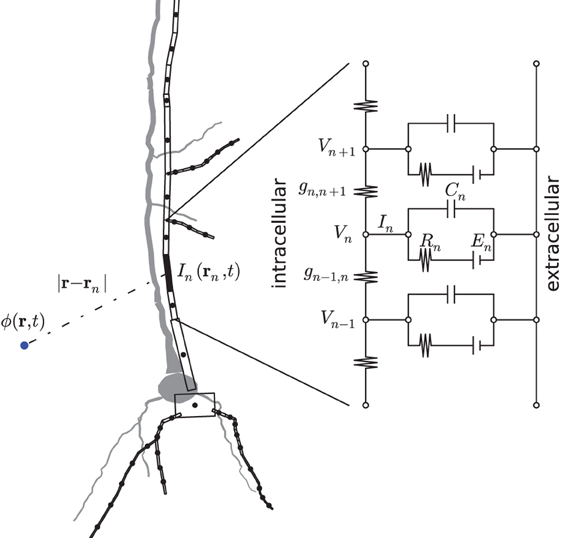
\includegraphics[width=0.7\linewidth]{Figures/linden2014_fig2A.png}
  \caption{Principle of compartment‑based forward modeling.
           Each compartment (index $n$) is treated as a point current
           source at position $\mathbf r_n$, and the potential at an
           electrode $\mathbf r$ is 
           ${\displaystyle \phi(\mathbf r)=\sum_n
           \frac{I_n}{4\pi\sigma|\mathbf r-\mathbf r_n|}}$. This is the same as equation \ref{eq:pointSource} but for a specific timestep. 
           \textit{Reproduced from} Lindén \emph{et al.}\ (2014), Fig.~2A,
           \href{https://creativecommons.org/licenses/by/4.0/}{CC‑BY 4.0}.}
  \label{fig:compartment_forward_linden}
\end{figure}

Each compartment in the neuron model contributes to the extracellular potential as a point current source or sink. Under the standard volume conductor assumptions, the contribution from a small compartment $n$ at position $\mathbf{r}_n$ to the potential at an observation point $\mathbf{r}$ (e.g., an electrode) is given by the classical formula:

\begin{equation}
\phi_n(\mathbf{r}, t) = \frac{1}{4\pi\sigma} \frac{I_n(t)}{\lvert \mathbf{r} - \mathbf{r}_n \rvert},
\label{eq:pointSource}
\end{equation}

where $I_n(t)$ is the time-varying \textit{transmembrane current} leaving compartment $n$ into the extracellular space, and $\sigma$ is the electrical conductivity of the surrounding medium (assumed constant). This relationship is a consequence of \textit{volume conductor theory} in the quasi-static regime: at EEG frequencies, inductive and capacitive displacement effects in tissue are negligible, so the extracellular space behaves like an ohmic (purely resistive) medium \cite{Nunez2006}.

In such a medium, the electric potential satisfies Poisson’s equation $\nabla \cdot (\sigma \nabla \phi) = -I_{\text{ext}}$, whose solution in an infinite homogeneous volume leads to a $1/r$ dependence. Figure \ref{fig:compartment_forward_linden} illustrates this compartment-based forward modeling setup: each compartment acts as a point source at location $\mathbf{r}_n$, and an electrode at position $\mathbf{r}$ sees a contribution $\phi_n$ that decays with the inverse distance. Because the tissue is approximately linear (ohmic), contributions from all compartments \textit{superpose linearly}. Thus, the total extracellular potential $\phi(\mathbf{r},t)$ at the electrode is the sum of contributions from all $N$ compartments of all active neurons:

\begin{equation}
\phi(\mathbf{r}, t) = \frac{1}{4\pi\sigma} \sum_{n=1}^{N} \frac{I_n(t)}{\lvert \mathbf{r} - \mathbf{r}_n \rvert}.
\label{eq:superposition}
\end{equation}

This formula (a summation of Coulomb-like contributions) is the core of forward modeling of brain potentials. It inherently assumes a \textit{point-source approximation} for each compartment, meaning the compartment is treated as a point where current enters or leaves the extracellular space. In reality, neuronal compartments have finite length, so a more accurate model for nearby electrodes is the \textit{line-source integration} along the compartment’s length. The line-source model integrates the contribution of current distributed over the compartment and results in a modified expression that converges to the point-source formula at distances much larger than the compartment length. In practice, for electrodes that are far from the neuron (such as scalp EEG electrodes, which are centimeters away), the point-source approximation is usually very good and close to line-source models.

\subsubsection{Current Dipole Representation}

An important simplification in EEG forward modeling is the use of \textit{equivalent current dipoles} to represent distributed neural sources. In essence, a group of nearby source–sink pairs can be mathematically summarized by a single dipole moment vector $\mathbf{p}$, which is the first-order term in a multipole expansion of the current distribution. For example, a single neuron’s transmembrane currents, which include many tiny sources and sinks, have an overall dipole moment that can be computed by summing $I_n \mathbf{r}_n$ over all compartments (with appropriate reference). The \textit{dipole-based} (DB) forward model assumes that this net dipole (or a collection of dipoles) is the source for EEG, rather than tracking every compartment. This approximation is widely used in EEG source modeling, especially for representing synchronous activity in a patch of cortex.

The rationale is that at sufficiently large distances (far-field), the detailed multi-polar structure of the source is not resolved – the field from a complex source distribution will fall off as if it were a single dipole to first order. Indeed, computational studies have found that for electrodes on the scalp, a neuron’s full compartment model and its equivalent dipole produce very similar EEG signals \cite{Næss2015}. Næss (2015) showed that a single neuron’s contribution to a distant electrode could be well-approximated by the neuron’s current dipole moment, with errors becoming negligible at distances of a few millimeters and beyond. This justifies the prevalent use of dipole sources in EEG forward models. However, it should be emphasized that the dipole model is an approximation. The dipole simplification fails to capture the true potential field. Thus, while we will often speak of “current dipoles” as the sources of EEG, one must remember this is a convenient summary of many distributed currents. 
Forward modeling of EEG signals involves simulating neural activity in biophysical neuron models and then computing the resulting scalp potentials via volume conduction theory. The compartmental modeling approach provides a detailed current source density for each neuron, which can be summed up (or simplified to dipoles) to predict the EEG. Thanks to the linearity of Maxwell’s equations in conductive media, contributions from many neurons superpose to generate the complex EEG waveforms observed. This theoretical framework – as laid out by Halnes et al. (2024) in \textit{Electric Brain Signals} – underpins the analyses in this thesis \cite{Halnes2024ElectricBrainSignals}.

\subsection{Current Dipole Moments and Their Limitations} \label{subsec: CDM limitations}

Electroencephalographic source modeling often relies on the \textit{equivalent current dipole} as a first-order approximation of distributed neural currents. In a multipole expansion of any localized current distribution with zero net charge, the dipole moment is the lowest-order (non-zero) term. Treating a cluster of neural sources as a point dipole greatly simplifies forward calculations and is justified under certain conditions. In particular, when the recording electrode is far from the neural source region (the \textit{far-field} regime), fine spatial details of the current distribution become indistinguishable. The distant electric field depends primarily on the total dipole moment rather than the exact arrangement of individual sources and sinks \cite{Halnes2024ElectricBrainSignals}. This is the basis for representing, e.g., an active cortical patch or a single neuron by a dipole vector $\mathbf{p}$ in EEG models \cite{Næss2015}. Even in realistic layered media (brain, cerebrospinal fluid, skull, scalp), the far-field condition holds: a localized current source can be replaced by an equivalent dipole without loss of accuracy in predicting scalp potentials, aside from overall scaling and smearing effects introduced by the layers \cite{Nunez2006}. Consequently, the equivalent dipole approximation is widely and successfully used in both EEG forward modeling and inverse source localization \cite{Nunez2006, Buzsaki2012}.

However, the current dipole approximation comes with important \textit{limitations}. As a point source model, it cannot capture the true spatial complexity of neural currents in the \textit{near-field} regime. When a recording electrode is very close to the generating neurons (as in intracortical recordings, electrocorticography (ECoG), or subdural grid electrodes), higher-order moments of the source distribution significantly influence the measured potential. In this regime, treating the source as a simple dipole can lead to large errors. Computational studies by Næss (2015) found that for electrodes within about a millimeter of a neuron (ECoG-like distances), the dipole model \emph{failed} to reproduce the compartment-based potentials, whereas at several millimeters it succeeded. In other words, a point dipole is too coarse a representation for near-field recordings, which are sensitive to the neuron's multipolar structure. The breakdown occurs because the electrode begins to “see” the separate contributions of current entering and leaving different parts of the neuron, rather than just the net effect. In such cases, contributions from higher-order terms (e.g. quadrupoles) do not cancel out and must be considered. For instance, a single pyramidal neuron with synaptic input at mid-apical dendrite can momentarily act like a current quadrupole: with a sink and source in close vertical proximity and opposite pairs of return currents. At a distance of 100 µm or 200~µm (typical ECoG electrode separation from cortex), these complex source geometries produce appreciable potential differences that a lone dipole cannot capture. Thus, while scalp EEG (far-field) can be modeled accurately enough with equivalent dipoles, subdural and intracortical recordings demand more detailed source models. This constraint is fundamentally tied to scale: if the spatial extent of the source is not negligible compared to the source-to-sensor distance, the dipole approximation will be incomplete. Notably, human cortical pyramidal cells are larger (they have longer apical dendrites) than those of smaller mammals, meaning their dipole lengths are greater and require even larger observation distances for the dipole model to remain valid. In summary, the dipole idealization holds for scalp EEG but loses accuracy for electrodes in close proximity to the neural generators, necessitating higher-fidelity modeling in those contexts \cite{Næss2015}.

Another limitation of the dipole moment model is that it implicitly assumes the dominant sources of EEG are arranged in an open-field dipolar configuration—historically identified with synchronous postsynaptic currents in aligned dendrites of cortical pyramidal neurons. This assumption leaves out other contributions that do not neatly sum into a single dipole. In reality, neurons generate currents across various compartments (soma, dendrites, and axon), and not all of these currents reinforce one another in the far-field. The classic view in EEG theory has been that action potential currents (largely flowing in axons and the soma) contribute minimally to scalp recordings. There are several reasons for this belief: a single action potential is extremely brief (1–2 ms) and produces rapidly changing source–sink configurations that tend to cancel out, effectively forming a small current loop (a closed field or higher-order multipole) whose distant field is weak. Additionally, spikes across neurons are typically asynchronous, and any high-frequency components they generate are strongly attenuated by tissue and skull filtering. As a result, traditional models focus on the lower-frequency, prolonged synaptic currents in dendrites as the primary generators of EEG signals \cite{Buzsaki2012}. In the dipole approximation framework, one essentially assumes that these dendritic currents create a net dipole and that other currents (e.g. those associated with axonal or somatic activity) either cancel out or are too small/fast to matter at the scalp. This simplifying assumption has been productive, but it is not universally accurate – especially for signals recorded nearer to the brain or when considering high-frequency EEG components. If a neuron’s non-dendritic currents do not align with the orientation of the dominant dipole (for example, if axonal currents form a different dipole or a more complex pattern), a single dipole moment might miss their effect entirely. In essence, the standard dipole model acts as a spatial low-pass filter: it captures the coarse, length-scale $\sim$1~cm contributions (the dendritic open-field currents) while filtering out finer-scale source patterns such as those from thin axonal processes or tightly coupled source-sink pairs. This is a reasonable approximation for classical scalp EEG rhythms (dominated by synchronous dendritic currents in cortical columns), but it may underrepresent phenomena where axonal currents play a role.

Recent evidence and theoretical developments suggest that these “hidden” contributions, though individually small, could become significant under certain conditions. For instance, when many neurons fire synchronously, the usually-cancelling fields from action potentials can summate to produce a detectable signal. Teleńczuk \textit{et al.} (2015) provided a striking demonstration of this: by averaging the epidural EEG signal time-locked to single cortical neuron spikes (spike-triggered averaging), they identified a reproducible waveform associated with an action potential \cite{Telenczuk2015}. This shows that even the rapid axonal and somatic currents of a spike can imprint on extracellular potentials if observed with sufficiently high bandwidth and proximity. Moreover, while the spike itself primarily generates high-frequency oscillations, the simultaneous return currents and afterpotentials can last up to tens of milliseconds, overlapping with the lower-frequency bands of EEG. These afterpotentials (e.g. the slow afterhyperpolarization following a burst of spikes) can produce field effects comparable in duration to synaptic currents and thus may contribute to what is traditionally considered the EEG frequency range. In light of such findings, the once-clear boundary between “dendritic (EEG-relevant) currents” and “axonal (EEG-irrelevant) currents” has started to blur. While it remains true that postsynaptic dendritic currents are the primary source of scalp EEG signals \cite{Buzsaki2012}, other sources are not strictly zero. Modeling work by Ness et al. (2016) and Halnes et al. (2024) further indicate that under conditions like strong synchronous firing or certain cellular configurations, membrane currents outside the dendrites (for example, currents in the axon initial segment or Nodes of Ranvier during action potentials) can measurably influence the local field \cite{ness2016subthreshold, Halnes2024ElectricBrainSignals}. These influences might be especially relevant for ECoG recordings or high-density EEG, where electrodes are closer to cortical sources or have higher sensitivity to fast transients. The conservative approach of using a single dipole per source, while robust for many purposes, could thus omit subtle but potentially important contributions from axonal pathways.

In summary, the current dipole moment is an extremely useful abstraction in EEG modeling – it encapsulates the essence of how distributed neural currents project to distant electrodes. It works well for far-field recordings in a volume conductor and provides a tractable link between neural activity and scalp signals. However, it is fundamentally a first-order approximation. Its validity deteriorates when the electrode is in the \emph{near field}––that is, when the source-to-sensor distance is not large relative to the linear dimensions of the current distribution––or when the generators contain appreciable higher-order multipole components.  A prototypical case is the axial and return currents that accompany a propagating action potential along a straight axon: their spatial pattern is predominantly \emph{quadrupolar}, so a single equivalent dipole cannot capture their contribution to the field \cite{McColgan2017}. This realization motivates the development of \textit{axon-aware} forward models and other higher-resolution approaches. By incorporating axonal currents and other higher-order effects into our forward model, we can improve the biological realism of EEG predictions. In practice, this could mean supplementing dipole models with additional source elements or using full multicompartment neuron models to compute contributions from dendrites \emph{and} axons. Embracing such complexity is especially important for bridging the gap between conventional EEG theory (focused on cortical columns as dipoles) and new research questions—like the one at the heart of this thesis—about the role of axonal activity. Indeed, as Halnes et al. (2024) emphasize, a comprehensive understanding of “electric brain signals” requires accounting for all major current-generating elements of neurons, not just dendritic synaptic currents \cite{Halnes2024ElectricBrainSignals}. Therefore, having acknowledged the strengths and weaknesses of the dipole approximation, we now turn our attention to the specific contributions of axons to extracellular potentials.

\subsection{Axonal Contributions to EEG Signals}\label{subsec:AxonalContributions}

Section \ref{subsec: CDM limitations} highlighted that the prevailing \emph{current dipole approximation} – which aggregates neuronal currents into an equivalent dipole at the soma – succeeds for far-field predictions under certain assumptions, but it neglects the extended structure of neurons. In particular, conventional EEG models often ignore \emph{axonal} currents, assuming their contributions to scalp signals are negligible. This assumption stems from the fact that action potentials (APs) in axons are extremely brief (1–2 ms) and form traveling source–sink pairs whose fields tend to cancel out at a distance. In essence, a single myelinated axon spike generates a closely spaced sink at an active node of Ranvier and source in the adjacent internodes (due to return current), approximating a small current quadrupole. Unless many such events occur in unison, the net far-field effect averages out. Thus, for decades EEG theory has emphasized postsynaptic dendritic currents as the dominant generators of EEG signals, treating axonal spikes as inconsequential noise \cite{McColgan2017}. Indeed, presynaptic terminal currents (at axon endings) have been estimated to require astronomically large numbers of synchronous events to register at the scalp (on the order of $10^{12}$ terminals for a 100~nA·m signal), underscoring why they are usually omitted in forward models \cite{Thio2023}.

Nevertheless, a growing body of evidence – theoretical, computational and experimental – now suggests that under specific conditions, axonal contributions to EEG signals can become significant \cite{Thio2023, McColgan2017, Brake2025}. A key insight is that the impact of any neuronal current on the EEG critically depends on the spatial organization and temporal synchrony of the sources. If axonal currents are synchronously activated across many neurons with a favorable geometry, their contributions can constructively sum rather than cancel. For example, modeling work by \textcite{Murakami2006} demonstrated that synchronous firing of on the order of $10^4$ cortical neurons could produce appreciable far-field signals. In their simulations, action potential bursts in a local population (layer V pyramidal neurons) contributed up to $\sim$20\% of the total EEG dipole moment, with the remaining $\sim$80\% coming from postsynaptic currents. This challenges the old notion that spikes contribute only a negligible fraction. The large contribution in such models arises because the spike currents were synchronized in time and aligned in space (since pyramidal cell axon initial segments are roughly parallel and normal to the cortical surface, like their dendrites). Under these conditions, the extracellular fields from individual axons no longer cancel out, but instead add up coherently.

The geometry of axonal arbors also plays a crucial role in determining their field effect. When many axons terminate in the same locale, they can form an effective current dipole layer. A theoretical and experimental study by \textcite{McColgan2017} showed that an \emph{axonal terminal zone} – a region where numerous axons branch and end in close proximity – can generate a prominent dipolar field in the surrounding medium. Their model of the avian auditory brainstem (nucleus laminaris) predicted a polarity inversion across the terminal layer: synaptic termini acted as a synchronized current sink, while the portions of axons proximal to the termini served as distributed current sources due to return currents flowing out of the axonal membrane. This source–sink configuration produces a clear dipole field pattern, much like a classic postsynaptic dipole but generated by axonal activity. Notably, the low-frequency component of the signal (below $\sim$1~kHz, reflecting the slower envelope of the compound spike activity) carried most of the dipole moment and radiated to the far field. Higher-frequency components associated with the fast AP upstroke, on the other hand, attenuated rapidly with distance. These findings were confirmed by multi-electrode recordings \emph{in vivo} in the owl brainstem: the observed local field potentials showed the predicted dipolar profile and amplitude, demonstrating that synchronized axonal spikes can indeed produce mesoscopic field potentials of considerable strength. In contrast, when axonal currents lack such organization e.g., if axons fire at random times or their orientations are uniformly distributed, their contributions will largely cancel out and appear as high-frequency noise, consistent with the negligible impact assumed in conventional models.

Another factor that can enhance axonal contributions is the presence of prolonged or repetitive spiking activity. An individual action potential is followed by afterpotentials (including the afterhyperpolarization) that last for tens of milliseconds, effectively extending the duration of the current imbalance. These afterpotentials generate slower varying currents comparable in duration to synaptic currents, and can therefore contribute power in the EEG-relevant frequency bands (tens of Hz or lower). \textcite{Bean2007} notes that post-spike afterhyperpolarizations can reach amplitudes similar to postsynaptic potentials, meaning a single spike is not purely a transient blip of current but has a significant low-frequency tail. If a neuron fires a burst of several spikes in quick succession, these afterpotential “tails” can overlap and summate, producing a more sustained dipole moment. Rhythmic high-frequency burst firing (for instance, a population of neurons firing spike bursts phase-locked to a theta rhythm) can thus generate an oscillatory field. Experimental observations have linked certain EEG oscillations to underlying spike bursts – for example, the high-frequency (“fast”) spindle oscillations during sleep are associated with rhythmic burst firing of cortical neurons. Similarly, increases in the EEG high-gamma band (60–200~Hz) correlate with heightened multi-neuron spiking activity. These correlations suggest that under conditions of synchrony, axonal spikes and their afterpotentials do imprint on extracellular signals. Recent computational work reinforces this point: \textcite{Brake2025} found that while isolated, asynchronous spikes contribute negligibly to the typical $1/f$ EEG background, synchronous spiking can produce detectable narrowband power at high frequencies (up to the hundreds of Hz). In their biophysical simulations, action potentials alone (in the absence of synaptic input) could generate measurable oscillatory signals when many neurons fired in synchrony, though the overall power contributed by spikes in normal conditions was only on the order of $\sim$1\% of the total EEG spectrum. Thus, axonal contributions tend to remain hidden unless there is either a high degree of synchronization or repeated firing that shifts some power into lower frequencies.

It is under extreme synchronous conditions that axonal signals become most apparent. In pathological states such as epilepsy, for instance, large neuronal ensembles may fire action potentials nearly simultaneously. The prototypical \emph{interictal epileptic spike} observed in EEG is a sharp voltage transient often followed by a slower wave. Computational models of epileptic discharges indicate that the fast “spike” component can result from the summated extracellular fields of many synchronous action potentials, whereas the subsequent slow wave reflects synaptic and intrinsic currents following the spike burst. In a neural network model replicating human hippocampal epileptic spikes, a brief synchronous burst of APs was required to produce the large-amplitude (~mV) transient observed in intracranial EEG, supporting the idea that pathologically high synchrony can drive spike-dominated field events. Even in less extreme scenarios, strong synaptic input can induce coherent spiking across a local population, effectively momentarily “boosting” the population dipole moment via axonal currents. In evoked responses (for example, the brainstem auditory evoked potential), the early peaks (latency <10 ms) are known to originate from synchronous volley-like firing in peripheral and brainstem axonal pathways, demonstrating that well-timed axonal activity can produce identifiable far-field signals.

In summary, while the quasi-static dipole approximation (centered on dendritic currents) is generally valid for EEG under typical conditions, there are important exceptions where axonal currents contribute non-negligibly. Theoretical analyses show that the synchrony of firing and the arrangement of axons can elevate spike contributions from a vanishingly small fraction to a significant portion of the source signal. Likewise, other's simulations and experiments confirm that action potentials – especially when occurring in bursts or in organized fiber tracts – can generate detectable EEG potentials. These findings motivate the development of \emph{axon-aware} forward models for EEG. By incorporating axonal geometry and active spike currents into our source models, we can improve the biological realism of EEG simulations. In the later sections these effects are investigated using my own simulations of neurons and axons.

\clearpage
\section{Methods}
To investigate the contribution of axons to measurable brain potentials, I compare the extracellular fields generated by canonical pyramidal neurons (Hay et al.) and isolated axons (Hallermann et al.). By simulating various population sizes and spatial configurations in LFPy, I aim to identify under which conditions axons may contribute significantly to ECoG or EEG signals.

\subsection{Computational Modeling Tools}

The simulations in this study were conducted using the NEURON simulation environment and the LFPy Python library, following a compartment-based forward modeling approach. NEURON served as the core engine for simulating neuronal dynamics, while LFPy was used on top of NEURON to calculate the resulting extracellular field potentials (local field potentials and EEG-like signals). I have not developed any new simulation libraries/tools; instead, I leveraged these established tools with their standard settings, as described below. Most code was adapted from or heavily inspired by the notebooks for figures from the \textit{Electric Brain Signals} book \cite{Halnes2024ElectricBrainSignals}. The code I've written and used for the simulation can be found in appendix \ref{app:simcode} as well as the GitHub repository associated with this thesis.

\subsubsection{NEURON Simulation Environment}
NEURON is a widely used simulation platform for modeling biophysical neurons with high anatomical detail \cite{Hines1997}. It allows neurons to be represented as multi-compartment cable models, in which each segment of the neuron is divided into small electrical compartments as explained in Section \ref{subsec: biophysical models}. NEURON numerically solves the membrane dynamics (ionic currents and membrane voltages) in each compartment by integrating the cable equations with Hodgkin--Huxley-type ion channel kinetics. This provides an accurate representation of how action potentials and synaptic potentials propagate throughout a neuron’s morphology. In my simulations, I imported morphologically detailed neuron models into NEURON via LFPy and used NEURON’s built-in mechanisms for membrane physiology (ion channels, passive properties, etc.). During each simulation, NEURON computed the transmembrane current $I_m(t)$ in every compartment at each time step. These transmembrane currents are the fundamental source signals that drive the extracellular potentials observed at electrodes.

\subsubsection{Extracellular Potential Calculation with LFPy}
LFPy is an open-source Python toolkit that runs on NEURON and enables forward-modeling of extracellular recordings \cite{Linden2014}. It provides high-level classes to set up neuron models, apply synaptic inputs, and place recording electrodes in the simulated extracellular space. Using LFPy, I instantiated the neuron model (\texttt{LFPy.Cell}) and attached synaptic input sources (\texttt{LFPy.Synapse}) to drive neuronal activity. I also defined an array of virtual recording electrodes (\texttt{LFPy.RecExtElectrode}) at specified locations in the simulation, at various distances above the neurons, to record the extracellular potential.

After running the NEURON simulation via LFPy’s \texttt{Cell.simulate()} method, LFPy computed the extracellular field by summing contributions from all compartments to each electrode’s potential. This calculation implements the standard volume-conductor formula: each compartment’s transmembrane current acts as a current source, contributing a potential $\phi_n = \frac{1}{4\pi\sigma}\frac{I_n(t)}{|\mathbf{r}-\mathbf{r}_n|}$ at an observation point $\mathbf{r}$, where $I_n(t)$ is the current in compartment $n$ and $\mathbf{r}_n$ its location \cite{Linden2014}. By superposing these contributions from every active compartment $n$, LFPy yields the total extracellular potential $\phi(\mathbf{r},t)$ at each electrode. In practice, LFPy’s implementation uses a line-source approximation (based on Holt and Koch 1999\cite{Holt1999}) for increased accuracy when electrodes are very close to the neuron, but for my purposes the simpler point-source model (all current emanating from the compartment center) was sufficient. The output of these calculations is a time series of voltage for each virtual electrode, effectively simulating the LFP or EEG signal that would be measured by those electrodes.

\subsubsection{Volume Conductor Assumptions}
The forward modeling in this thesis adopts the \emph{quasi-static volume-conductor approximation}. 
Brain tissue is treated as an infinite, homogeneous and isotropic \emph{ohmic} conductor with scalar conductivity $\sigma = 0.3\;\mathrm{S/m}$ (LFPy default). Under these assumptions displacement currents and inductive effects are negligible; hence the extracellular potential $\phi$ obeys
\begin{equation}
  \nabla\!\cdot\!\bigl(\sigma\nabla\phi\bigr) = \rho_{\text{ext}}, 
  \qquad\text{with}\qquad
  \mathbf{E} = -\nabla\phi .
  \label{eq:quasistatic}
\end{equation}
Because the medium is linear and time-invariant, the principle of superposition applies: 
the potentials produced by individual neuronal compartments can be summed to obtain the total potential at a recording point, as implemented in \texttt{RecExtElectrode} \cite{PlonseyHeppner1967,Hamalainen1993}.

I also assume a point-source representation for each compartment’s current, as noted above. That is, each compartment injects current into the extracellular space at a point (its center). This point-source approximation is inherent in the $1/(4\pi\sigma r)$ formula and is valid when the electrode is sufficiently far from the neuron that each compartment’s extent is negligible relative to the distance. For electrodes in very close proximity, a line-source model would be more accurate, but in this study most recording electrodes are placed either in the cortical near-field or far-field at distances where the point-source assumption holds well. Moreover, my simulations do not include complex head geometry or layered conductivity—rather, the focus is on the idealized case of an infinite uniform volume conductor. These assumptions are consistent with the established models in the literature for calculating LFP and EEG signals from neuronal activity \cite{Linden2014}. 

\subsubsection{Other Tools and Libraries Utilized}
My code relies on several different libraries for python. NumPy \cite{NumPy} was essential for controlling the data and saving simulations for plotting and analysis in the future. It is also a requirement for LFPy. Matplotlib \cite{Matplotlib} was used for the visualization of simulation data and for creating many of the figures in this thesis. SciPy \cite{SciPy} is also a dependency for LFPy, but it was not directly utilized in the newly written code for this thesis. 
I did not modify any source code of NEURON or LFPy. All simulations were performed using LFPy’s standard functions. By using these well-validated tools without custom modifications, I ensured that my results are directly comparable to prior studies and grounded in a tested modeling framework.

\subsection{Simulating Populations}\label{subsec:populationMethod}
For the simulations of populations of cells a density of 100 000 neurons/mm³ was used. This is in accordance with prevailing estimates of the average density of neurons in the mouse brain. Keller et al. found that the density of neurons was on average 92,616 cells/mm³ with a standard deviation of $\pm$ 25,000 cells/mm³ \cite{Keller2018densities}. This estimate was also used in a study by Thunemann et al. in simulating ECoG signals in mice to evaluate the validity of Windansee electrode grids \cite{Thunemann2022Windansee}.
In order to reduce the required computing power to run the simulations, the cell was only simulated one time and then copied according to the number of cells required in the population. The cells were placed in a cylinder with normally distributed positions around the center of the bottom of the cylinder as seen in Figure \ref{fig:popcylinder}. The radius of the cylinder was varied according to the population in order to keep the same density of the population. 
\newline
All cells were then moved together such that the tallest possible part of the tallest cell was 10 $\mu$m below the defined surface of the brain at 87 mm. This ensures that the closest electrode was always at least 10 $\mu$m above the population of cells. The cylinder the cells were distributed in had a constant height of 25 $\mu$m and the cells were uniformly distributed across this height-interval. As such all the cells were at most $10 \mu m + 25\mu m= 35\mu m$ down from the electrode. All cells also got a random rotation around the z axis, meaning all axons and apical dendrites always pointed radially out of the brain, but other parts of the cell were rotated around its central axis. The first cell was always placed at the bottom center of the cylinder and given a rotation of 0. New random populations were created for every simulation. Figures \ref{fig:popmorphs} and \ref{fig:Axonpopmorphs} show examples of different populations of Hay cells and axons used for some of the simulations.

\begin{figure} [h]
    \centering
        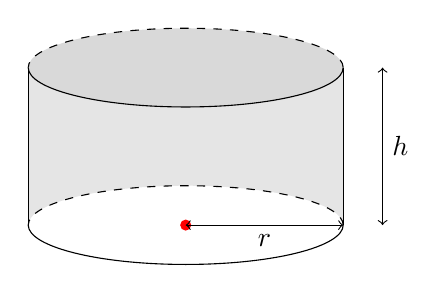
\begin{tikzpicture}[scale=1]
          % ------- parameters -------
          \def\R{2cm}      % radius
          \def\H{2cm}      % height  ( = \R )
          \def\EY{0.5cm}   % vertical radius of ellipses (perspective)
        
          % ------- cylinder side surface -------
          \path[fill=gray!20]
                (-\R,0) -- (-\R,\H)
                arc[start angle=180,end angle=360,
                    x radius=\R,y radius=\EY]
                -- (\R,0)
                arc[start angle=0,end angle=180,
                    x radius=\R,y radius=\EY]
                -- cycle;
        
          % ------- top disk -------
          \path[fill=gray!30]
                (-\R,\H) arc[start angle=180,end angle=180+360,
                             x radius=\R,y radius=\EY]
                -- cycle;
        
          % ------- outlines -------
          \draw (-\R,0) -- (-\R,\H);              % left edge
          \draw (\R,0)  -- (\R,\H);               % right edge
          \draw (-\R,\H) arc[start angle=180,end angle=360,
                             x radius=\R,y radius=\EY];       % front half, top
          \draw[dashed] (\R,\H) arc[start angle=0,end angle=180,
                                    x radius=\R,y radius=\EY]; % back half, top
          \draw (-\R,0) arc[start angle=180,end angle=360,
                            x radius=\R,y radius=\EY];        % front half, bottom
          \draw[dashed] (\R,0) arc[start angle=0,end angle=180,
                                   x radius=\R,y radius=\EY];  % back half, bottom
        
          % ------- center point -------
          \fill[red] (0,0) circle (2pt);
        
          % ------- radius and height arrows -------
          \draw[<->] (0,0) -- (\R,0)
                node[midway,below] {$r$};
          \draw[<->] (\R+0.5cm,0) -- ++(0,\H)
                node[midway,right] {$h$};
        \end{tikzpicture}
    \caption{Cylinder with constant height h and variable radius r. The red spot marks where the soma of the first cell is placed, and the others are normally distributed around this. For axons, the lowest segment was used in place of the soma (segment idx 0). See the functions \texttt{find\_pop\_radius} and \texttt{simulate} in appendix \ref{app:simcode} for more details.}
    \label{fig:popcylinder}
\end{figure}

\begin{figure}[htbp]
    \centering
    \makebox[\linewidth]{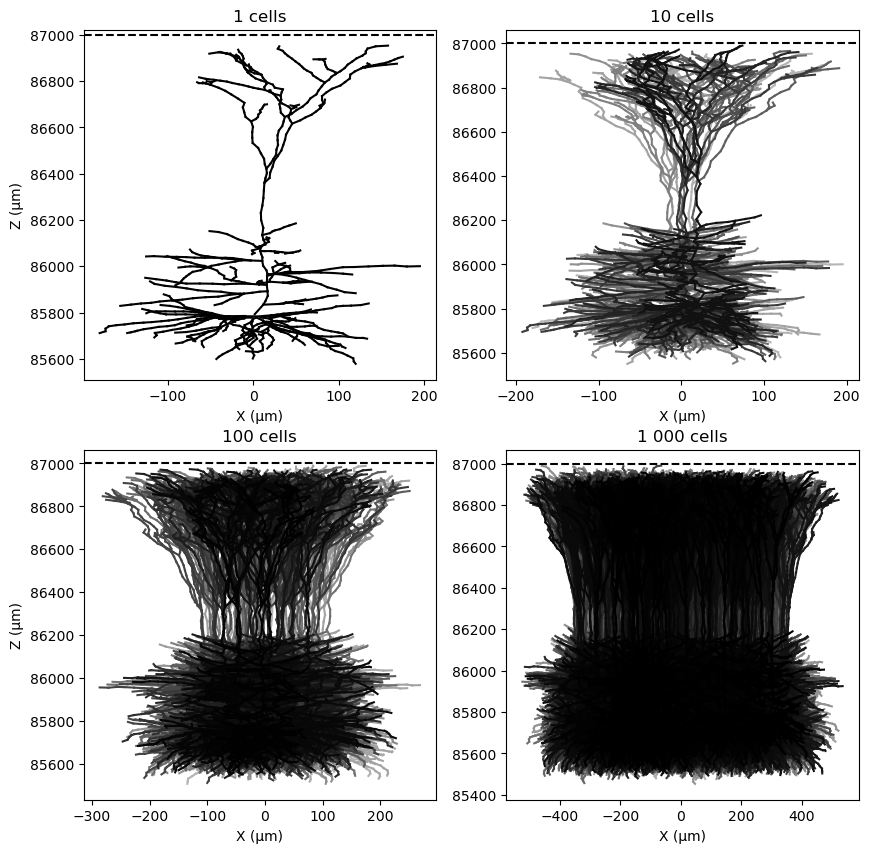
\includegraphics[width=1.2\linewidth]{Figures/popmorphs.png}}
    \caption{Example plot of the morphologies of different cell populations showing how populations of different sizes might look. Each population was created entirely for from scratch for their respective simulations. Each plot has all cells from the simulation plotted in the x and z direction where z is depth in the brain and x is the radial width. The stippled line at 87 000 $\mu m$ is the surface of the brain. The populations pictured are for complete cells from Hay et al. \cite{Hay2011}. The 10 000 cell population size is omitted for being too computationally expensive to plot.}
    \label{fig:popmorphs}
\end{figure}

\begin{figure}[htbp]
    \centering
    \makebox[\linewidth]{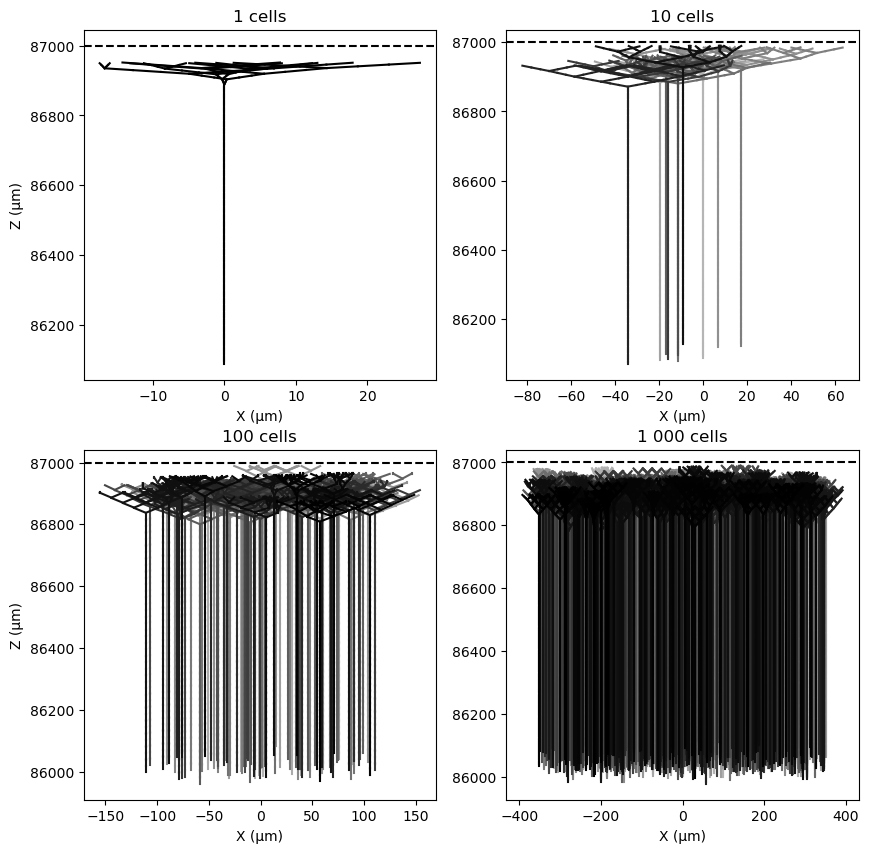
\includegraphics[width=1.2\linewidth]{Figures/AxonPopMorphs.png}}
    \caption{Same as Figure \ref{fig:popmorphs} but for axons.}
    \label{fig:Axonpopmorphs}
\end{figure}

\subsubsection{Changes Made During Testing} \label{subsubsec:CodeChanges}
After simulating all parameters with this code, the results seemed quite strange. Therefore, an adjustment was made to the code. Originally, \texttt{numpy.random.normal()} was used to get population offsets for height. Furthermore, the tallest cell was always placed 10 $\mu$ below the surface of the brain. This had the unfortunate side effect that the depth of the cells in each population varied greatly. As a consequence, the measured potentials were a lot lower than expected because of the greater distance. For simulations used in the results and the rest of this thesis the method to pick heights was changed to \texttt{numpy.random.uniform()}. The first cell was also always placed in the center of the population and 10 $\mu$m + the height of the population down from the surface level of the brain. As such, the scaling effects of larger populations were more predictable and realistic. See NumPy documentation for more details \cite{numpyDocumentation}.

\subsection{Electrode Placement}\label{subsec:Electrodes}
For all simulations, a set of electrodes was used to take measurements of the evoked potentials. The electrodes were placed at varying distances above the cell populations centered in the center of the disc the populations were distributed across. All electrodes were simulated with the same extracellular conductivity of 0.3 $S/m$ using the LFPy \texttt{RecExtElectrode} class. This class uses a simplified point source model for computing extracellular potentials. Some simulations also used the \newline \texttt{FourSphereVolumeConductor} class. This class takes into account the different conductivities of different tissues when calculating the resulting signal. These distances and conductivities can be found in Table \ref{tab:foursphereparams}. Figure \ref{fig:elecpos} shows the placement of the electrodes above an example population. The different distances were pseudo-logarithmically spaced as described in Table \ref{tab:elecdist}. The closest and furthest electrodes approximate ECoG and EEG respectively. The distances used were based on earlier simulations by Næss et al. 2021 \cite{Naess2021} and approximations derived from Slutzky et al. \cite{Slutzky2010}.

\begin{table}[h]
    \centering
    \begin{tabular}{|c|c|c|}
        \hline
        Tissue type & conductance (S/m) & thickness (mm) \\
        \hline
        Brain & 0.276 & 87 \\
        \hline
        CSF & 1.65 & 2 \\
        \hline
        Skull & 0.01 & 5 \\
        \hline
        Scalp & 0.465 & 5 \\
        \hline
    \end{tabular}
    \caption{Parameters used for the \texttt{FourSphereVolumeConductor} class electrode. Note that the class takes radii as an input and not thicknesses as is expressed in this table.}
    \label{tab:foursphereparams}
\end{table}

\begin{table}[h]
    \centering
    \begin{tabular}{|c|c|}
        \hline
         Electrode number & Distance in $\mu$m  \\
         \hline
         1 (ECoG) & 10  \\
         \hline
         2 & 30 \\
         \hline
         3 & 100    \\
         \hline
         4 & 300 \\
         \hline
         5 & 6000 \\
         \hline
         6 (EEG) & 12 000 (12 mm) \\
         \hline
         7 (EEG with sphere approximation) & 12 000 (12 mm)\\
         \hline
         8 (EEG with FourSphere) & 12 000 (12 mm) \\
         \hline
    \end{tabular}
    \caption{Distances from the top of the highest axon in the population where electrodes were placed. Electrodes 1 and 2 are in the ECoG range while electrodes 6, 7, and 8 are in approximate locations for EEG electrodes.}
    \label{tab:elecdist}
\end{table}

\begin{figure}
    \centering
    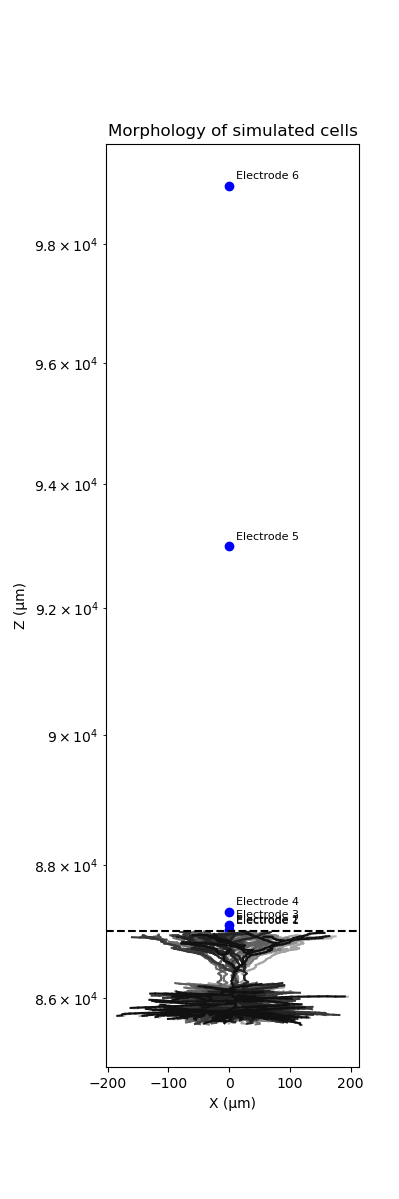
\includegraphics[width=0.5\linewidth]{Figures/Elecpos.png}
    \caption{Diagram of placement of electrodes above a population of 10 Hay pyramidal cells. Each blue dot is an electrode and at the furthest electrode both the EEG-like high conductivity \texttt{RecExtElectrode} and \texttt{FourSphereVolumeConductor} electrodes are placed.}
    \label{fig:elecpos}
\end{figure}
\subsubsection{Finding Conductance for Four Sphere Approximation} \label{subsubsec: find sigma}
The \texttt{FourSphereVolumeConductor} class should be a more accurate electrode, but it is very computationally expensive. In order to speed up simulations, this electrode was omitted for the larger populations (all populations where n\_cells >= 100). Instead, a \texttt{RecExtElectrode} class electrode was used with a different conductance in order to approximate the \texttt{FourSphereVolumeConductor} electrode. To approximate a layered volume conductor as a single homogeneous medium, an adjusted value for the conductance was found by placing the two types of electrodes at the same spot and simulating different conductances until a relatively closely matching signal was achieved. Through this trial and error process, a value of 1 $S/m$ was found to approximate the four sphere model for all cell models utilized in this thesis. This simplified value reflects the dominant attenuating effect of the skull, which has been shown to lower scalp potentials by an order of magnitude compared to intracranial recordings. An electrode with this higher assumed conductivity was placed in the same locations as the furthest electrode (12 mm).
This hybrid approach allows realistic modeling of both near- and far-field extracellular potentials while maintaining compatibility with simulations sensitive to fine-scale contributions from axons and spikes, and also being computationally light enough to simulate.

\subsubsection{Calculating Equivalent Conductance for Four Sphere Approximation} \label{subsubsec: calc sigma}
A different way to approximate a layered volume conductor is by using an equivalent conductivity calculated from the conductivities of the layers. In this section, I calculate an effective conductivity that preserves the same total resistance across the structure. Assuming a one-dimensional geometry with constant cross-sectional area, the resistance of each layer \( R_i \) per unit area is given by:
\begin{equation}
    R_i = \frac{l_i}{\sigma_i},
\end{equation}
where \( l_i \) is the thickness of the \( i \)-th layer (in meters) and \( \sigma_i \) is its conductivity (in siemens per meter, S/m).

The total resistance per unit area for layers connected in series is:
\begin{equation}
    R_{\text{total}} = \sum_{i=1}^{4} R_i = \sum_{i=1}^{4} \frac{l_i}{\sigma_i}.
\end{equation}

The effective conductivity \( \sigma_{\text{eq}} \) of a single homogeneous layer with total thickness \( l_{\text{total}} \) is then:
\begin{equation}
    \sigma_{\text{eq}} = \frac{l_{\text{total}}}{R_{\text{total}}},
\end{equation}
where
\begin{equation}
    l_{\text{total}} = \sum_{i=1}^{4} l_i.
\end{equation}

Given the parameters of approximate thicknesses for different parts of the head (see Figure \ref{fig:modalities} from Hagen et al. 2018\cite{Hagen2018}) and conductances from figure 1.1 in \textit{Electric Brain Signals} \cite{Hagen_ElectricBrainSignals_repo}:
\begin{align*}
    \text{Layer Thicknesses:} \quad & l = [1000, 1000, 5000, 5000]\ \mu\text{m} = [0.001, 0.001, 0.005, 0.005]\ \text{m}, \\
    \text{Conductivities:} \quad & \sigma = [0.276, 1.65, 0.01, 0.465]\ \text{S/m},
\end{align*}
the resistances of the individual layers are:
\begin{align*}
    R_1 &= \frac{0.001}{0.276} = 0.0036232\ \Omega\cdot \text{m}^2, \\
    R_2 &= \frac{0.001}{1.65} = 0.0006061\ \Omega\cdot \text{m}^2, \\
    R_3 &= \frac{0.005}{0.01} = 0.5\ \Omega\cdot \text{m}^2, \\
    R_4 &= \frac{0.005}{0.465} = 0.0107527\ \Omega\cdot \text{m}^2.
\end{align*}

Thus, the total resistance per unit area is:
\begin{equation}
    R_{\text{total}} = 0.0036232 + 0.0006061 + 0.5 + 0.0107527 = 0.51498\ \Omega\cdot \text{m}^2,
\end{equation}
and the total thickness is:
\begin{equation}
    l_{\text{total}} = 0.001 + 0.001 + 0.005 + 0.005 = 0.012\ \text{m}.
\end{equation}

The effective conductivity is then:
\begin{equation}
    \sigma_{\text{eq}} = \frac{0.012}{0.51498} \approx 0.0233\ \text{S/m}.
\end{equation}

Hence, the homogenized medium can be approximated with an effective conductivity of:
\begin{equation}
    \boxed{ \sigma_{\text{eq}} \approx 0.0233\ \text{S/m} }.
\end{equation}

In order to be on the safe side, this was rounded down to 0.02 $S/m$ for use in simulations. This simplified value reflects the dominant attenuating effect of the skull, which has been shown to lower scalp potentials by an order of magnitude compared to intracranial recordings. Electrodes with this lower assumed conductivity were placed in the same locations as the furthest electrode (12 mm). 

\subsection{Comparing Cell Models}\label{subsec:cellmodels}
Two different cell models were used for the simulations used in this thesis. For the effects of complete cells a layer 5 pyramidal neuron modeled by Hay et al. was used \cite{Hay2011}. This model was chosen for its state-of-the-art accuracy in real active processes and its accurate morphology \cite{ness2016subthreshold}. The model was also widely used for the simulations in the \textit{Electric Brain Signals} book \cite{Halnes2024ElectricBrainSignals}.

For axonal simulations a part of the Hallermann cell model was used \cite{Hallermann2012}. The authors of \textit{Electric Brain Signals} have coded a method to extract only the axon of the cell and included it in the repository for the code of the examples used in the book \cite{Hagen_ElectricBrainSignals_repo}. The same method and cell model was used in this thesis for axon-focused simulations. This was done in order to isolate the axonal contribution to the measured brain potentials. 

Both the Hallermann and Hay cells are models based on layer 5 pyramidal cells in the rat visual cortex \cite{Hallermann2012, Hay2011}. The two models focus on different aspects of cell function. Hay et al. focus on dendritic integration and spike backpropagation, whereas Hallermann et al. focuses on energy efficiency and axonal activity. This makes each model suitable for its respective simulations. The different configurations of each cell can be found in their respective constructor functions in appendix \ref{app:simcode} and were as follows:

\subsubsection{Passive Hay Soma (\texttt{hay\_soma})}
\label{sec:passive_hay_soma}
A full Hay pyramidal morphology but with all active channels disabled (purely passive membrane). A single fast \texttt{Exp2Syn} synapse (weight \(0.1\), \(\tau_1 = 0.1\ \mathrm{ms}\), \(\tau_2 = 1\ \mathrm{ms}\)) was placed at the soma (segment index 0) with an input at \(5\ \mathrm{ms}\). This configuration isolates the purely postsynaptic current generated by a somatic input under AMPA‐like kinetics. Using a passive cell ensures that no action potential is initiated in this case.

\subsubsection{Hallermann Axon (\texttt{hallermann\_axon})}
\label{sec:hallermann_axon}
The Hallermann et al.\ (2012) axon model was used in two variants: unmyelinated and myelinated. A brief current pulse (0.05 nA for 0.3 ms) was injected into the axon hillock (segment index~0) to trigger a spike. This configuration tests how axonal spike currents alone contribute to the extracellular signal.

\subsubsection{Hay Single Apical Dendritic Input (\texttt{hay\_single\_apical\_exp})}
\label{subsubsec:hay_single_apical}
This configuration reuses the Hay et al. (2011) morphology (passive) but places one Exp2Syn synapse (weight 0.1) at a randomly chosen apical dendritic segment ($700<z<\infty$ µm) with a spike at 5 ms.  It tests the minimal dipole generated by a distal input to quantify how single tuft events contribute to local and far‐field potentials.

\subsubsection{Distributed Apical Tuft Drive (\texttt{hay\_apical})}
\label{sec:hay_apical}
Using the passive Hay morphology, ten small \texttt{Exp2Syn} synapses (each weight \(0.01\)) were distributed over the apical tuft (segments with (z > 700\ $\mu$m) and activated simultaneously at (5 ms). This configuration simulates a strong, synchronous distal drive, as might occur during cortical UP-states or synchronized sensory input to layer~1. The reduced per-synapse weight maintains a reasonable total conductance while avoiding saturation of the cell.

\subsubsection{Active Hay Soma Model (\texttt{hay\_active\_soma})}
\label{subsubsec:hay_active_soma}
Finally, I restore the full set of active conductances in the Hay cell (voltage‐gated Na\textsuperscript{+}, K\textsuperscript{+}, etc.) and place an Exp2Syn synapse at the soma (weight 0.1, 5 ms). This tests how intrinsic action‐potential currents interact with synaptic inputs in shaping extracellular signals.

\subsection*{}
Each configuration was simulated under identical volume conductor assumptions, allowing us to compare the magnitude and waveform of the extracellular potentials they produce. Together, these setups isolate purely passive somatic input, axonal spikes (with or without myelin), localized distal dendritic input, distributed tuft input, and active-soma spiking.

\subsection{Combined Cell Models} \label{subsubsec:combinedcell}
In order to simulate more realistic combined signals, the Hallermann axon and the Hay cell were combined. This was inspired by an article from Rossel et al., more specifically Figure 1D in their article \cite{ROSSEL2023}. Here the authors theorize that the small positive deflection before the larger negative deflection is the AP-spike while the longer negative deflection is the PSPs. Figure \ref{fig:rossel} is taken directly from their article and will serve as the target signal for these simulations for ECoG-like electrodes. 
Technically, this was done by placing the two cells in the same location for x and y, as well as placing them the same distance from the brain surface level. This placement is illustrated in Figure \ref{fig:combinedmorph}. The \texttt{hallermann\_axon} was activated as soon as the simulation started, and then the synapses of the \texttt{hay\_apical} model were activated after a set delay to allow for the spike to propagate up the axon. This approximates two neurons connected through 10 synapses in the apical dendrites of the pyramidal neuron. The delay between firing was the time for the spike to propagate, plus an additional 1 ms to account for delay in the synapse. When measuring these combined cells, the axon and the cell were measured in their own array to enable scaling and shifting later. This was done in order to account for synapse weighting after the fact, in place of searching for a fitting weight. The axon signals were scaled by a factor of $2$ for measurements with a population size of 10,000 and myelinated axons to approximate the signals from Rossel et al. \cite{ROSSEL2023}. For unmyelinated axons, the scaling was left at $1$. To get closer to the signature from Figure \ref{fig:rossel} the 1 ms delay was also removed by shifting the spike closer to the activation of the synapses. More details can be found in the \texttt{runcombined} function in Appendix \ref{app:simcode}.

\begin{figure}[htbp]
    \centering
    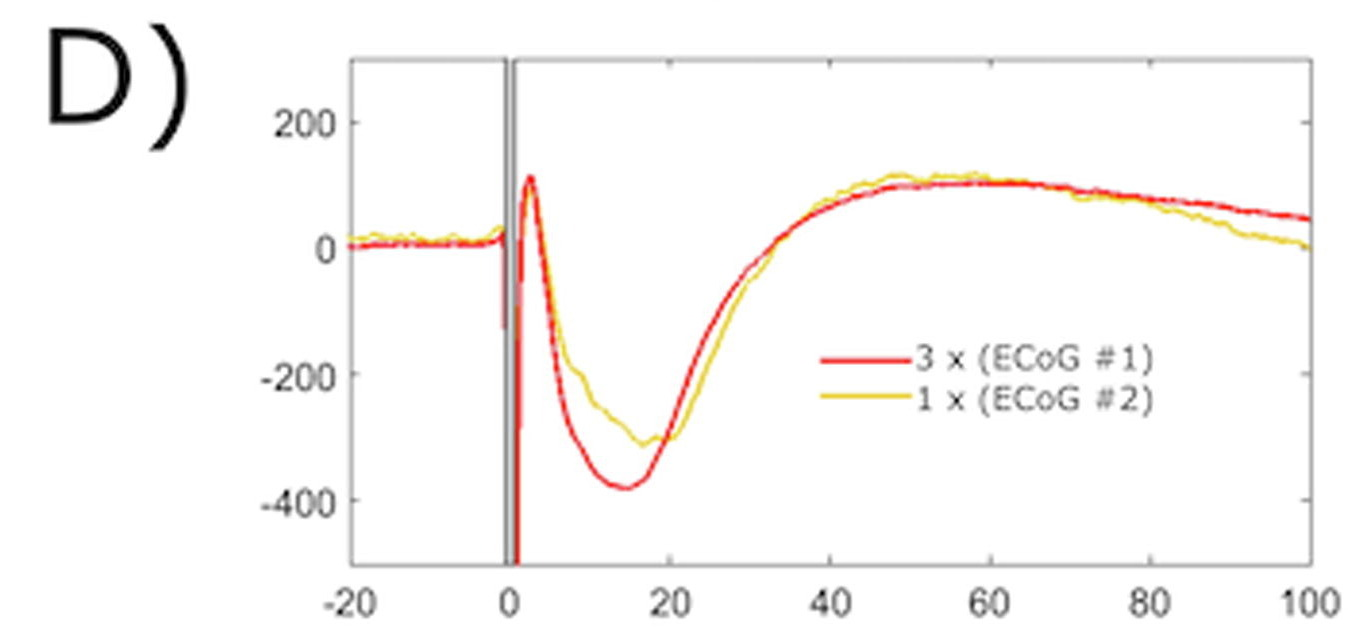
\includegraphics[width=\linewidth]{Figures/Rosselfig1d.jpg}
    \caption[ACEP waveform hotspot (Rossel et al., 2023) ]{%
    Figure 1D from Rossel et al. (2023) illustrating the hotspot waveform of an axono-cortical evoked potential.%
    \footnotesize Reprinted from Rossel et al. \cite{ROSSEL2023} Reproduced under the STM permissions guidelines.
    }
    \label{fig:rossel}
\end{figure}

\begin{figure}[htbp]
    \centering
    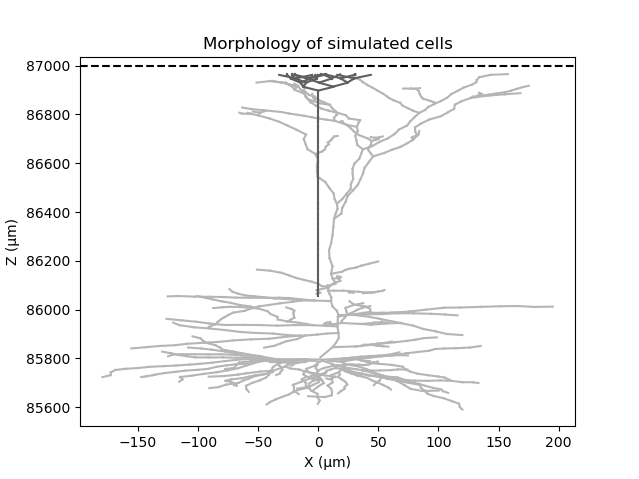
\includegraphics[width=\linewidth]{Figures/singlecombined.png}
    \caption{The morphology of the axon and hay cell as used in the combined plots. the straight line with bifurcations on the top is the axon while the larger cell behind is the complete Hay pyramidal cell.}
    \label{fig:combinedmorph}
\end{figure}

\newpage
\subsection{Use of AI Tools}
This thesis has been developed with the assistance of Artificial Intelligence (AI)-based tools, in accordance with the \textit{Guidelines for Use of Artificial Intelligence at NMBU}. The following tools have been used:

\begin{itemize}
    \item \textbf{ChatGPT:} ChatGPT is an AI-powered language model developed by OpenAI that functions as a conversational tool capable of generating human-like text, answering questions, and assisting with a wide range of writing and communication tasks. It was used as a writing aid to improve structure, clarity, and academic tone. Suggestions were critically evaluated, and the final text was reviewed and validated by the author. ChatGPT was not used to generate factual content or original research material. ChatGPT was also used in a fact-finding capacity to find relevant sources in addition to working through citations in both earlier masters theses and textbooks for relevant courses at NMBU.
    
    \item \textbf{Writefull (Overleaf integration):} Writefull is an AI-based language tool designed to improve academic and scientific writing by providing grammar corrections, language suggestions, and automated feedback, and it is specifically tailored for use in research contexts. The tool is based on ChatGPT and includes a custom prompt and offers suggestions on the fly. Used for language polishing, including grammar correction and fluency improvements. This tool is integrated in the online LaTeX editor Overleaf. 
    
    \item \textbf{GitHub Copilot:} GitHub Copilot is an AI-powered code completion tool developed by GitHub and OpenAI that assists programmers by suggesting code snippets, functions, and syntax in real time based on the context of the code being written. It was used as a programming assistant for code development. It provided syntax and structural suggestions, but the author reviewed, modified, and verified all final code.
\end{itemize}

No AI tool was used as a source of academic facts or literature. All cited material originates from verifiable, peer-reviewed sources or scientific databases. My research methods were entirely developed by me under the guidance of my supervisors. 

\clearpage
\section{Results}
\subsection{Approximations of FourSphere Electrodes}
When trying to approximate the \texttt{FourSphereVolumeConductor} electrodes with the two different methods mentioned in Section \ref{subsubsec: find sigma} and Section \ref{subsubsec: calc sigma} the resulting signals can be seen in Figure \ref{fig:FourSphereComp}. The resulting maximum amplitudes can also be seen in Table \ref{tab:FourSphereAmps}. The results showed a clear difference between the different approximations and the proper \texttt{FourSphereVolumeConductor}. For this, simulation a complete Hay cell was used with somatic excitatory input from a single synapse. Note that active processes were disabled for this simulation. 

\begin{figure}[h]
    \centering
    \makebox[\linewidth]{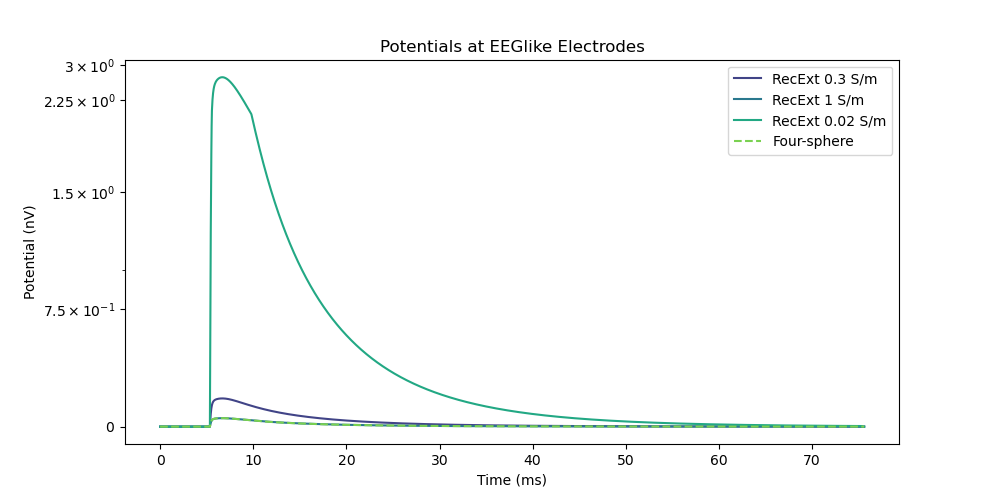
\includegraphics[width=1.2\linewidth]{Figures/Potentials_at_EEGlike.png}}
    \caption{Potential read from the different types of approximations of the \newline\texttt{FourSphereVolumeConductor} electrode and the actual measurement with the four sphere model. The stippled line shows the four sphere model and closely follows the trace from \texttt{RecExtElectrode} using a sigma of 1 $S/m$. Here a \texttt{hay\_soma} cell was used, meaning a single somatic input on a passive membrane cell.}
    \label{fig:FourSphereComp}
\end{figure}

\begin{table}[h]
    \centering
        \begin{tabular}{|c|c|c|c|}
        \hline
        Electrode type & Conductance ($S/m$) & Max Potential (nV) \\
        \hline
        \texttt{RecExtElectrode} & 0.3 & 0.181 \\
        \hline
        \texttt{RecExtElectrode} & 1 & 0.054 \\
        \hline
        \texttt{RecExtElectrode} & 0.02 & 2.708 \\
        \hline
        \texttt{FourSphereVolumeConductor} & n/a & 0.054 \\
        \hline
    \end{tabular}
    \caption{Max amplitudes measured by the different approximations of the \newline\texttt{FourSphereVolumeConductor} electrode and the actual measurement.}
    \label{tab:FourSphereAmps}
\end{table}

\newpage
\subsection{Chosen Waveforms for Varying Populations}\label{subsec:waveforms}
This section outlines some chosen waveforms of different cell models and how they change with populations of somewhat synchronized neurons. For these simulations, the jitter SD was 2 ms. Figure \ref{fig:apicalwav} outlines the waveforms for the \texttt{hay\_apical} cell. The signal is mostly negative with a tiny positive spike first. When summing, these tiny spikes are still visible for population sizes up to and including 100 cells. After this, the positive part is drowned by the vastly more outstretched negative potential. There is relatively little difference in the shape of the signal for the different populations.

Figure \ref{fig:axonwavmyen} shows the same waveforms for different population sizes of the Hallermann axon. The jitter time is still 2 ms and as with the apical input Hay cells the closest electrode is considered. Here the single action potential spike is very apparent, but already at 10 axons the max amplitude decreases and the signal gets more difficult to discern. Interestingly, the waveform from 10 000 axons starts to look more like the signal from a single AP than for population sizes in between. The larger population also achieves the same peak to peak amplitude as a single axon. This trend also mostly applies to unmyelinated axons, as shown in Figure \ref{fig:axonwavunmyen}. A key difference here is that the waveforms are a bit smoother and the amplitudes are higher than for the myelinated axon. 

\begin{figure}[htbp]
    \centering
    \makebox[\linewidth]{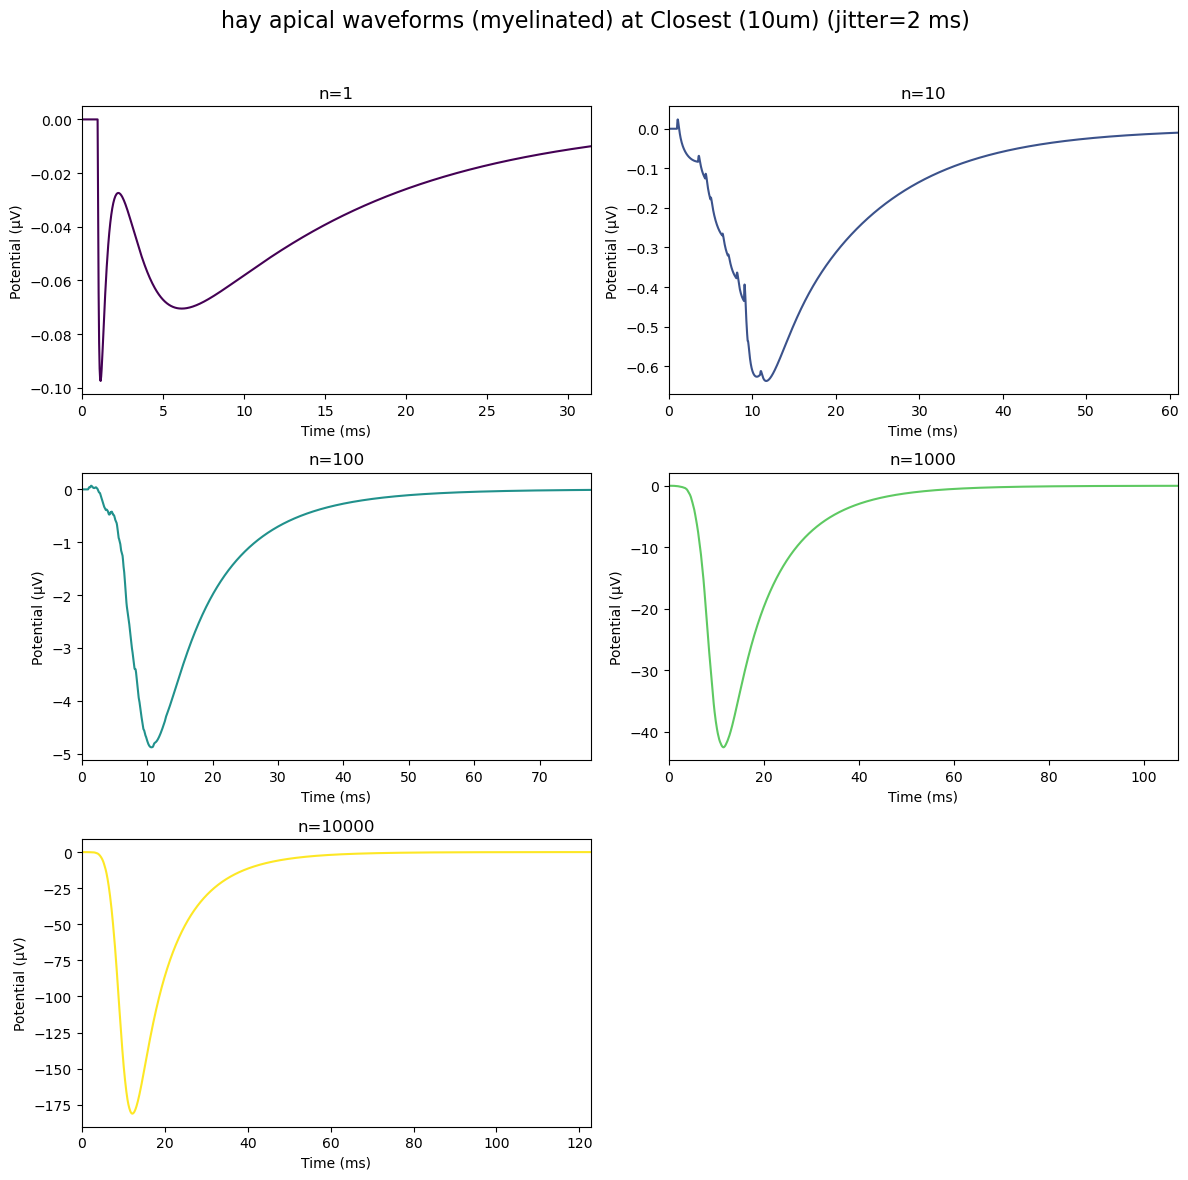
\includegraphics[width=1.2\linewidth]{Figures/Apical2jitter10um.png}}
    \caption{Waveforms for the \texttt{hay\_apical} cell model at the closest electrode (10 $\mu$m) and for a jitter SD of 2 ms.}
    \label{fig:apicalwav}
\end{figure}

\begin{figure}[htbp]
    \centering
    \makebox[1\linewidth]{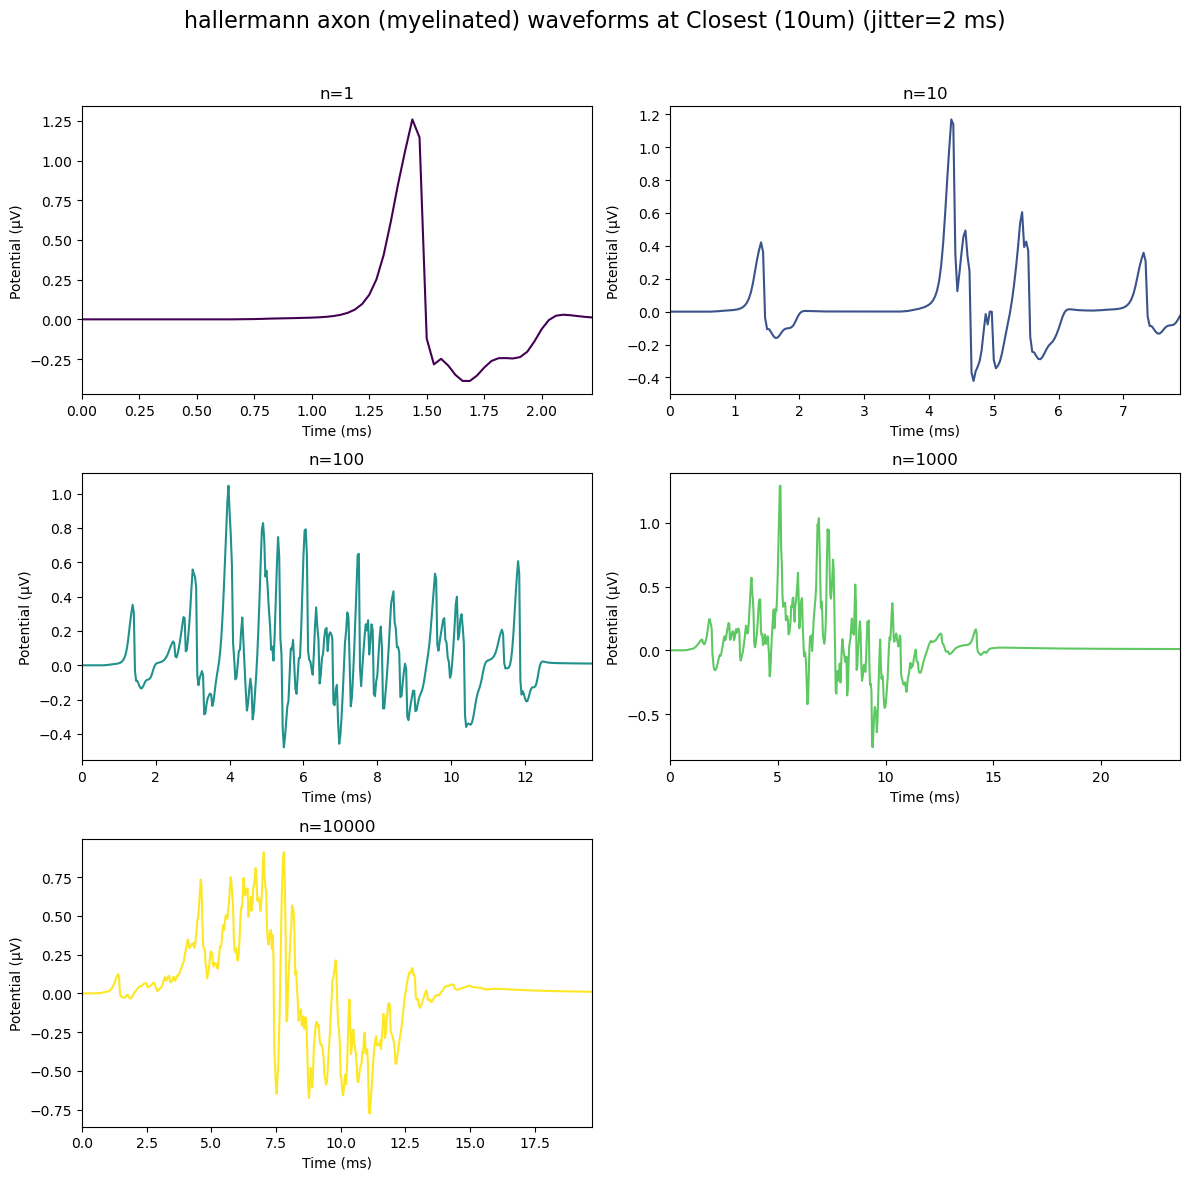
\includegraphics[width=1.2\linewidth]{Figures/Axon2jitter10um.png}}
    \caption{Waveforms for the \texttt{hallermann\_axon} cell model with myelination at the closest electrode (10 $\mu$m) and for a jitter SD of 2 ms.} 
    \label{fig:axonwavmyen}
\end{figure}

\begin{figure}[htbp]
    \centering
    \makebox[1\linewidth]{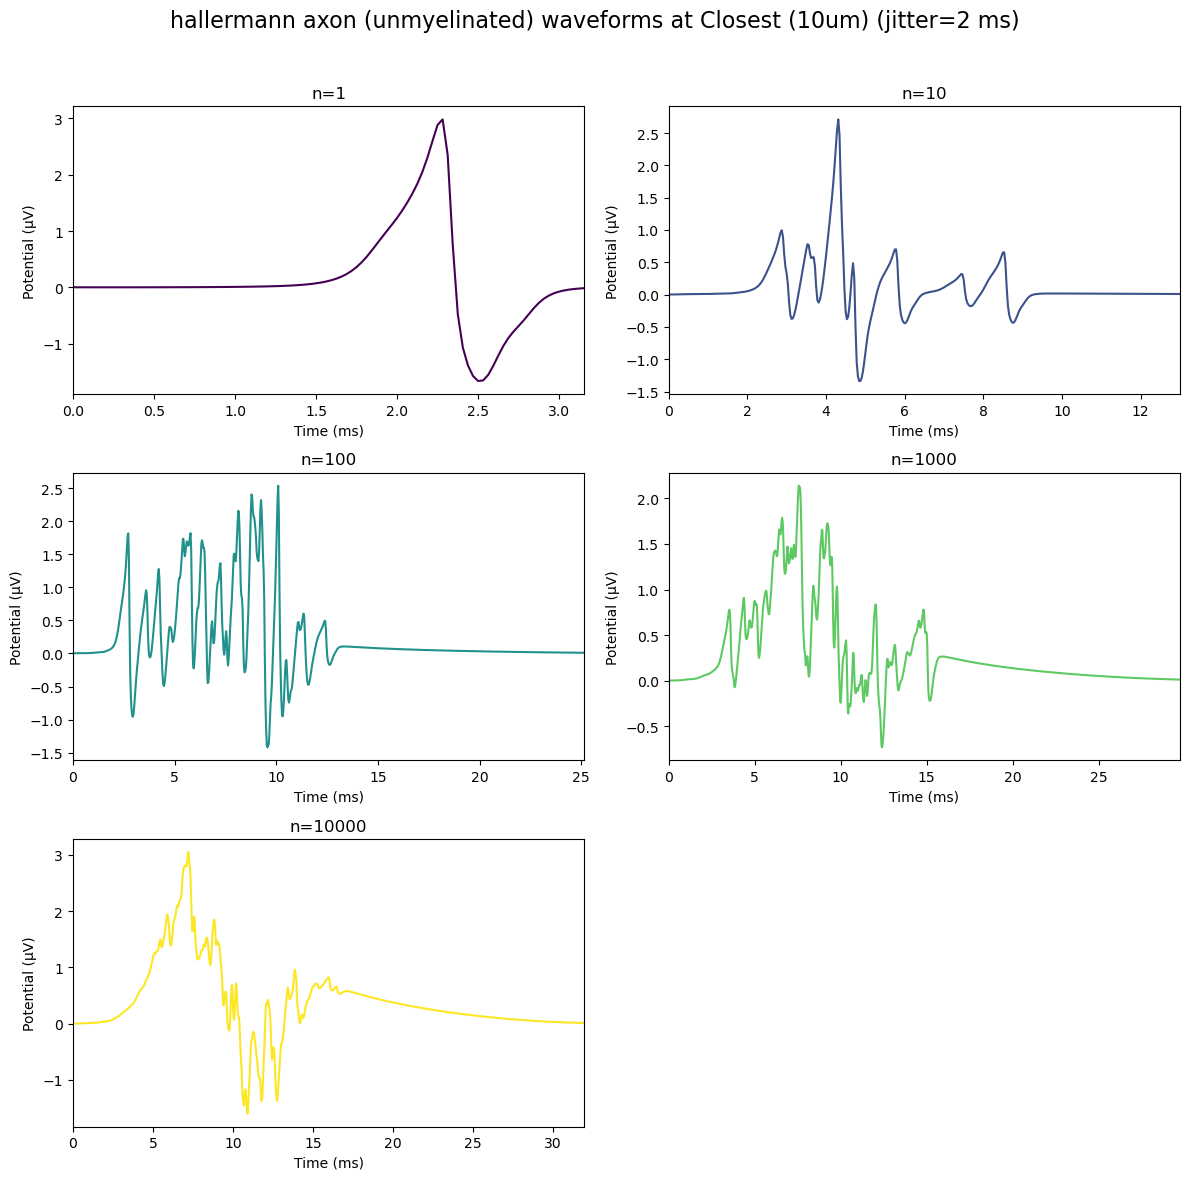
\includegraphics[width=1.2\linewidth]{Figures/Axon2jitter10umunmyen.png}}
    \caption{Waveforms for the \texttt{hallermann\_axon} cell model without myelination at the closest electrode (10 $\mu$m) and for a jitter SD of 2 ms.} 
    \label{fig:axonwavunmyen}
\end{figure}

\subsection{Effects of Distance on Axonal Potentials}
Figure \ref{fig:axonmyenelecswav} shows the waveforms of all electrodes used to measure a population of 10 000 axons with a 0 ms jitter value. The shapes of the waveforms are mostly the same, but the amplitudes are decreasing with increasing electrode number. Equivalently this means a larger distance from the cell to the electrode leads to lower potential measured. 

\begin{figure}[h]
    \centering
    \makebox[\linewidth]{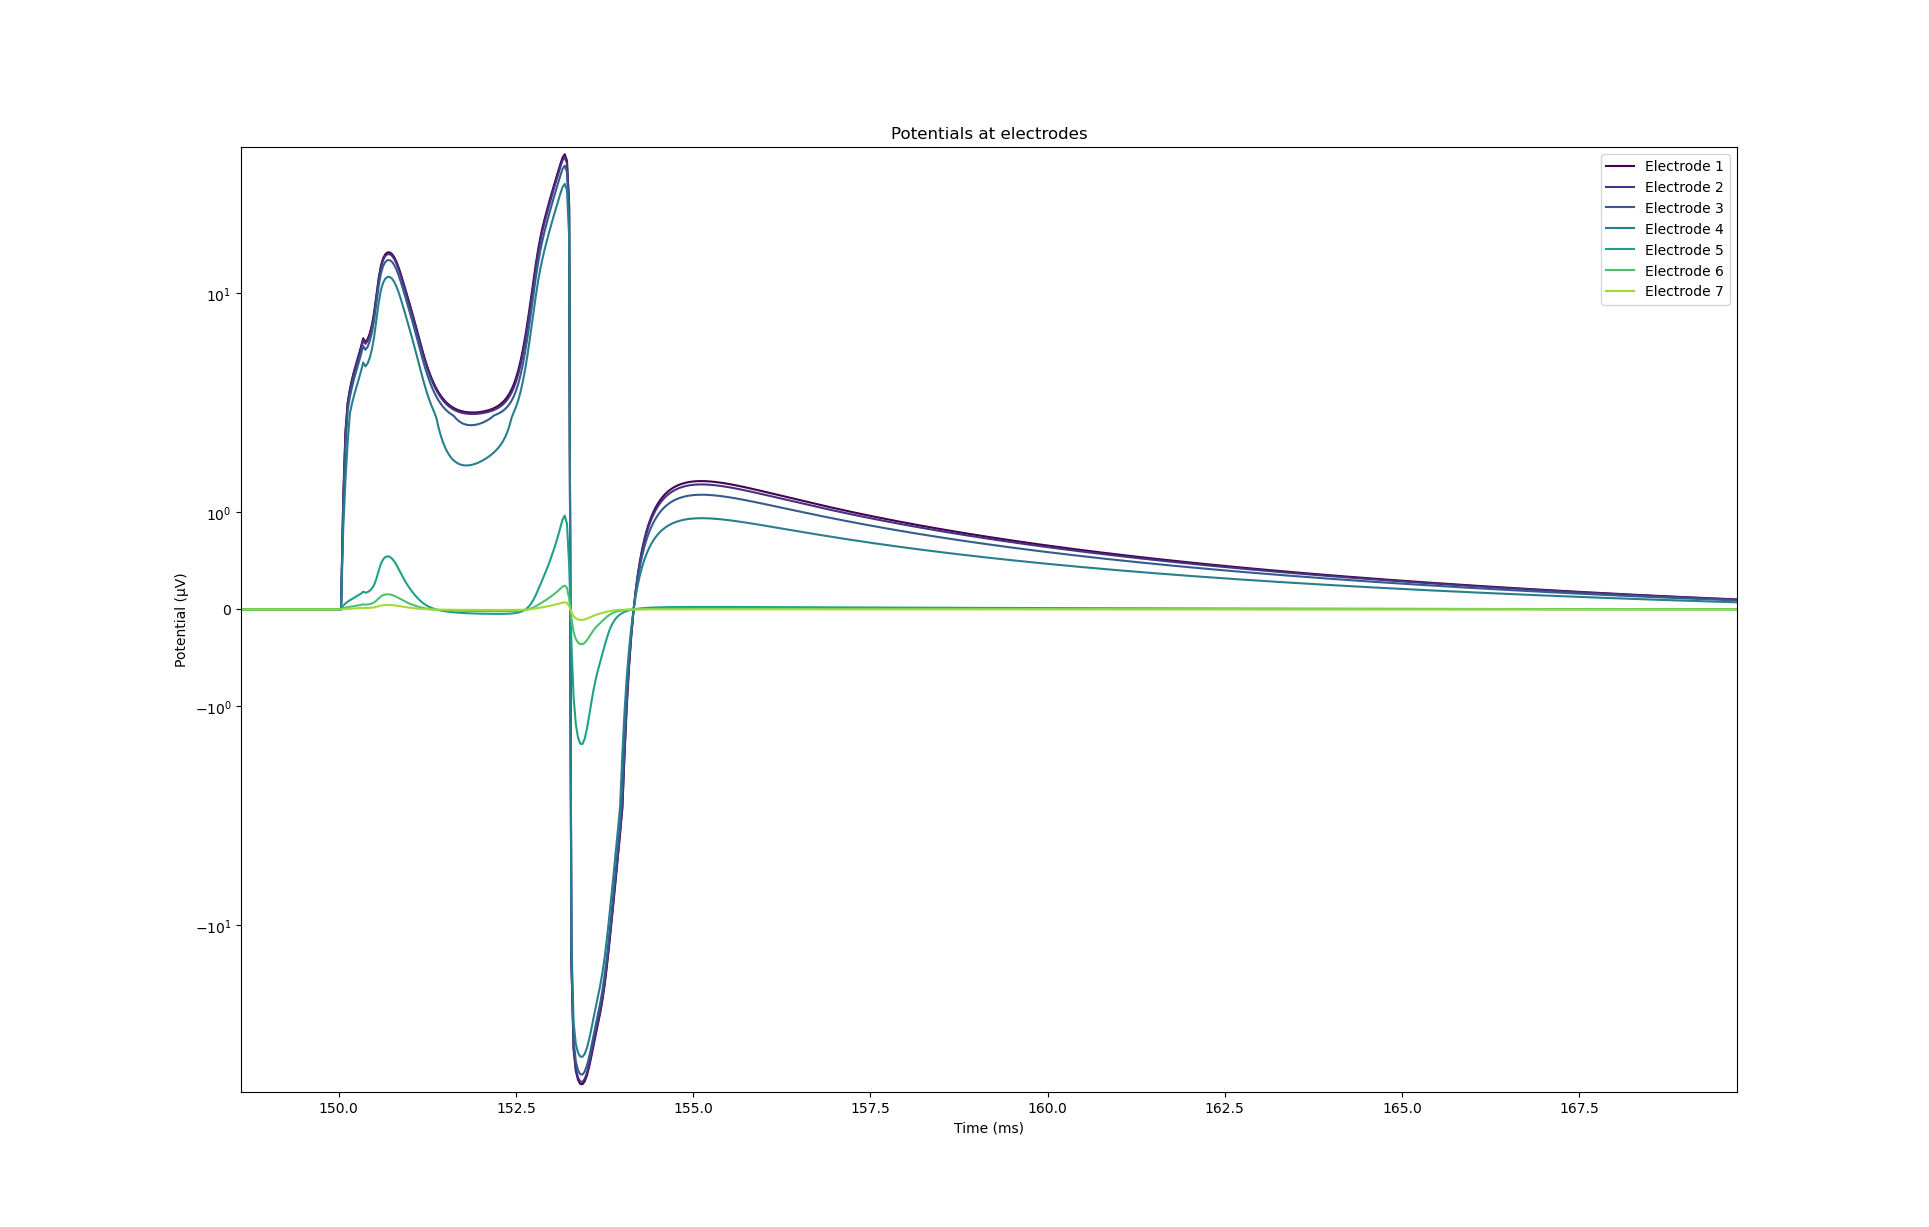
\includegraphics[width=1.2\linewidth]{Figures/axonunmyenpotselecs.png}}
    \caption{Waveforms of 10 000 unmyelinated axons with 0 jitter measured at all the different electrodes. The y-axis is logarithmic}
    \label{fig:axonmyenelecswav}
\end{figure}

\subsection{Temporal Smearing of Signals From Axons}
Figures \ref{fig:axonjitters} and \ref{fig:axonjitters2} show the waveforms of populations of 10 000 axons that are unmyelinated and measured with the electrode at 10 $\mu$m. The waveform for 0 jitter is clean and readable, but the higher jitter values become more and more chaotic. The amplitude plummets from around 140 $\mu$V at 0 ms jitter to around 12 $\mu$V at 1 ms jitter. The amplitudes keep falling for increasing jitter, plateauing at around 4 $\mu$V. Increasing the jitter also increases the "width" of the signals, or in other words, increases the length of time the signal is visible. Where no jitter yields a signal length on the order of 2-4 ms, the 10 ms jittered signal has a length of around 60 ms. 

\begin{figure}[htbp]
    \centering
    \vspace*{-3cm}
    \makebox[1\linewidth]{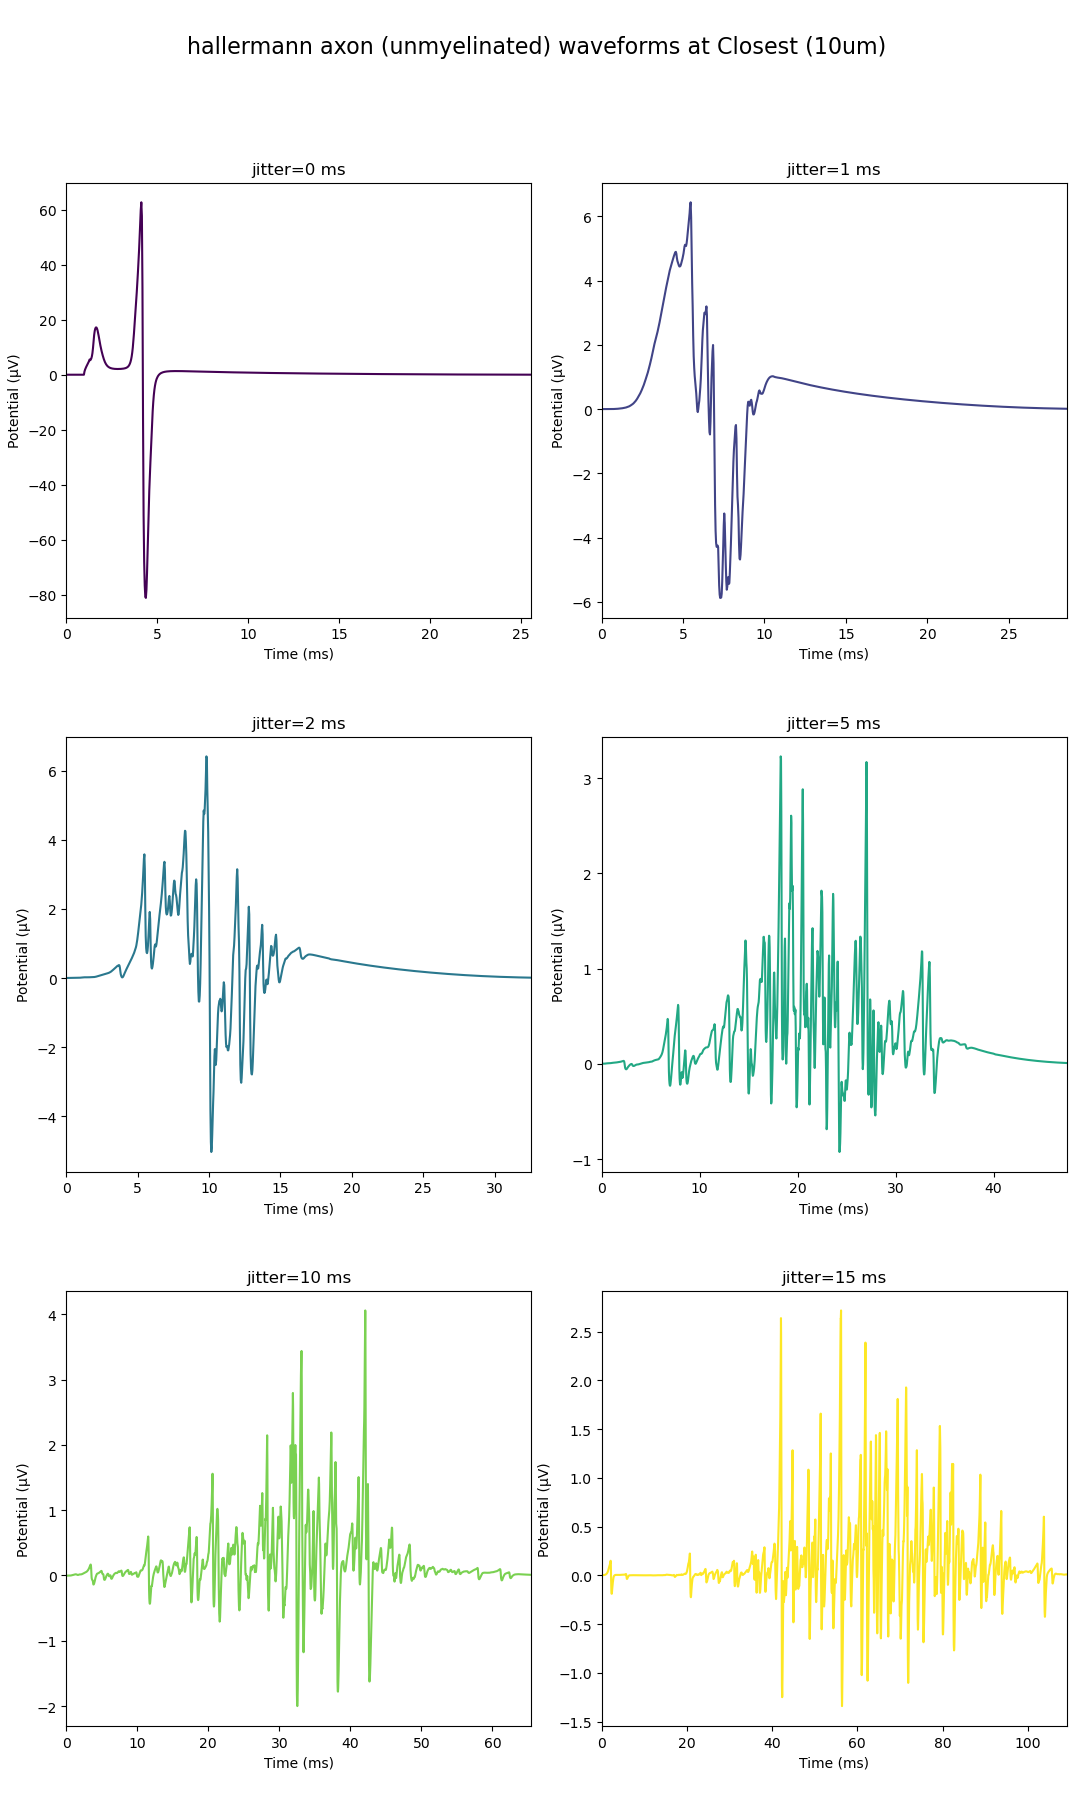
\includegraphics[width=1.2\linewidth]{Figures/axonjitters.png}}
    \caption{Waveforms for the \texttt{hallermann\_axon} cell model without myelination at the closest electrode (10 $\mu$m) and a population size of 10 000 with different jitter.} 
    \label{fig:axonjitters}
\end{figure}

\begin{figure}[htbp]
    \centering
    \vspace*{-3cm}
    \makebox[1\linewidth]{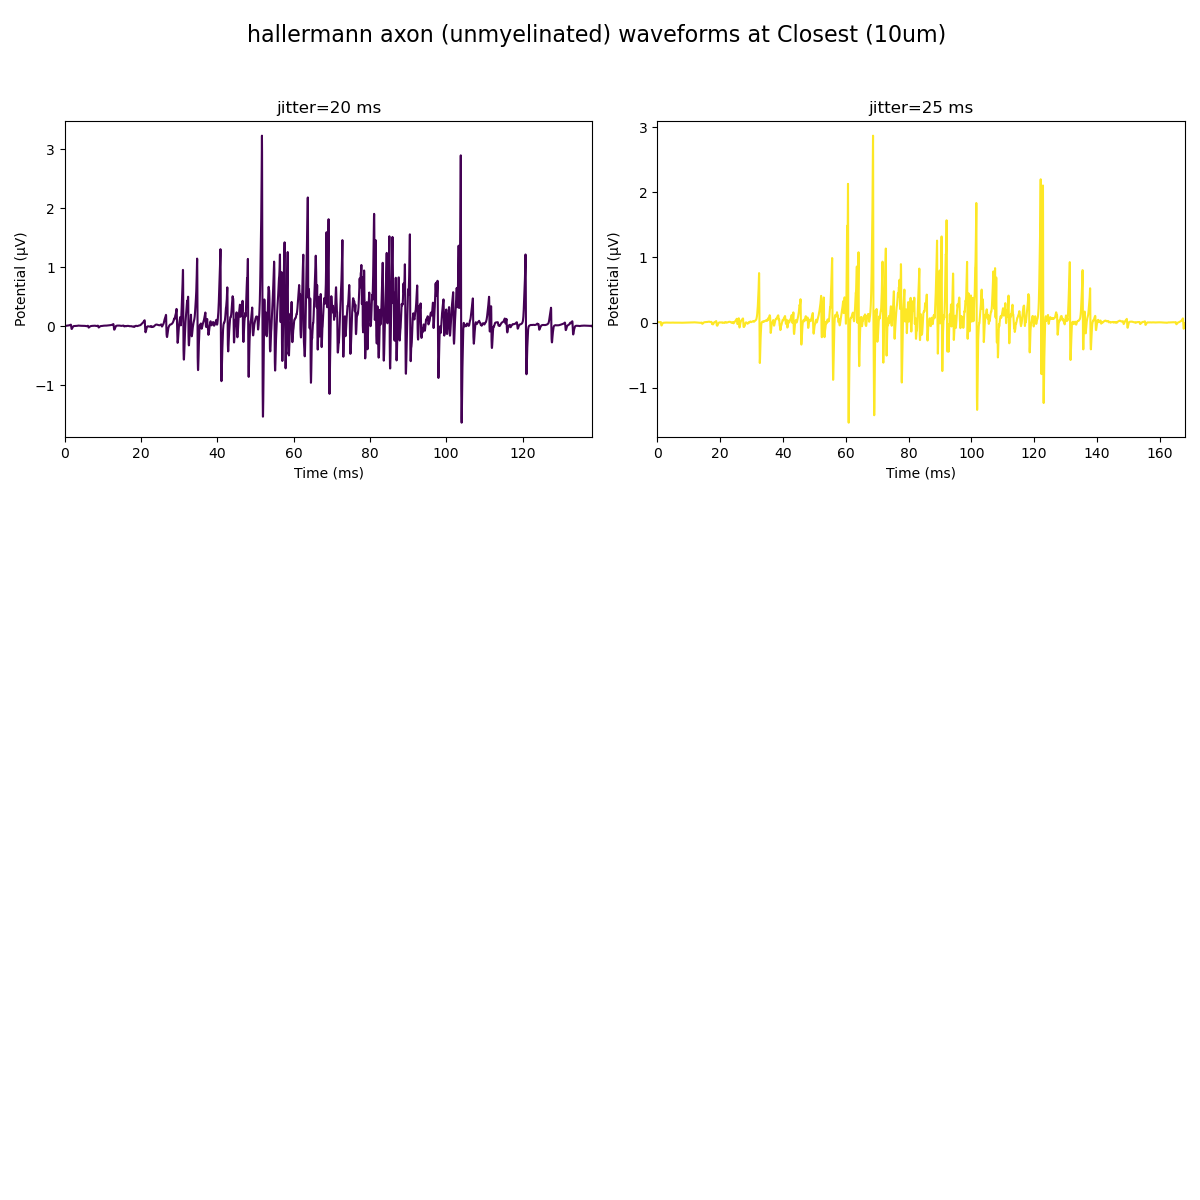
\includegraphics[width=1.2\linewidth]{Figures/axonjitters2.png}}
    \caption{(Continued) Waveforms for the \texttt{hallermann\_axon} cell model without myelination at the closest electrode (10 $\mu$m) and a population size of 10 000 with different jitter.}  
    \label{fig:axonjitters2}
\end{figure}

Figures \ref{fig:axonjitterseeg} and \ref{fig:axonjitters2eeg} show the same waveforms but for the furthest EEG-like electrode at 12 mm and with a higher conductance. Here the 0 ms jitter case has two clear spikes and a negative spike afterwards. At 1 ms and 2 ms jitter the signal is still discernible, but the amplitude has rapidly fallen. From 5 ms jitter and onwards, the signal looks just like random noise. The width of these waveforms seem to increase at about the same pace as the waveforms for the near field recording. 

\begin{figure}[htbp]
    \centering
    \vspace*{-3cm}
    \makebox[1\linewidth]{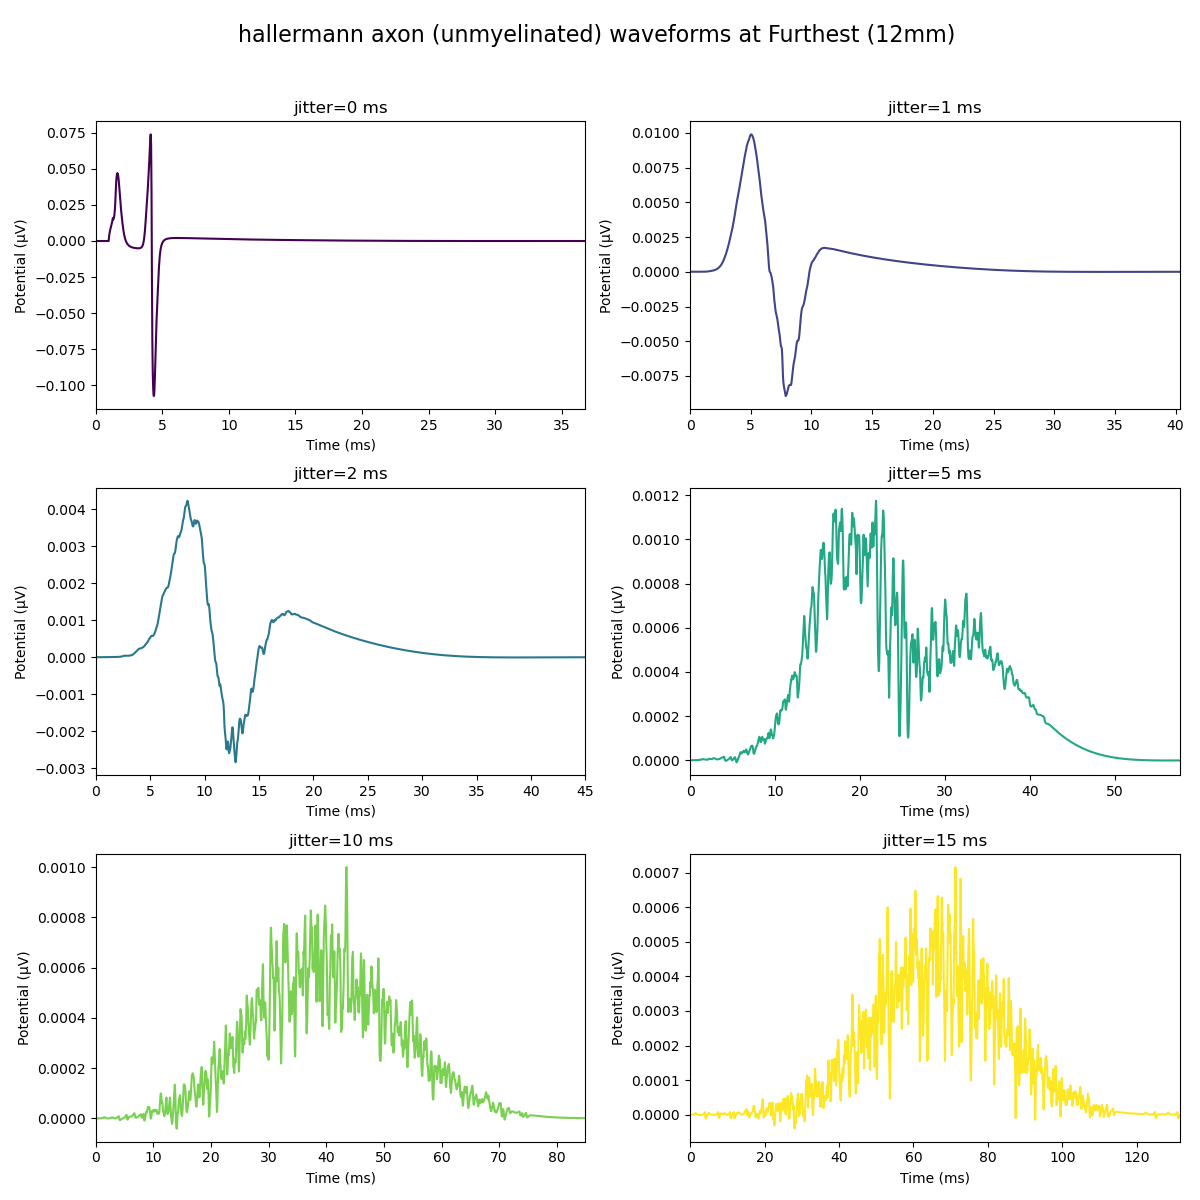
\includegraphics[width=1.2\linewidth]{Figures/axonjittersEEG.png}}
    \caption{Waveforms for the \texttt{hallermann\_axon} cell model without myelination at the furthest electrode (12 mm) with a higher EEG-like conductance and a population size of 10 000 with different jitter.} 
    \label{fig:axonjitterseeg}
\end{figure}

\begin{figure}[htbp]
    \centering
    \vspace*{-3cm}
    \makebox[1\linewidth]{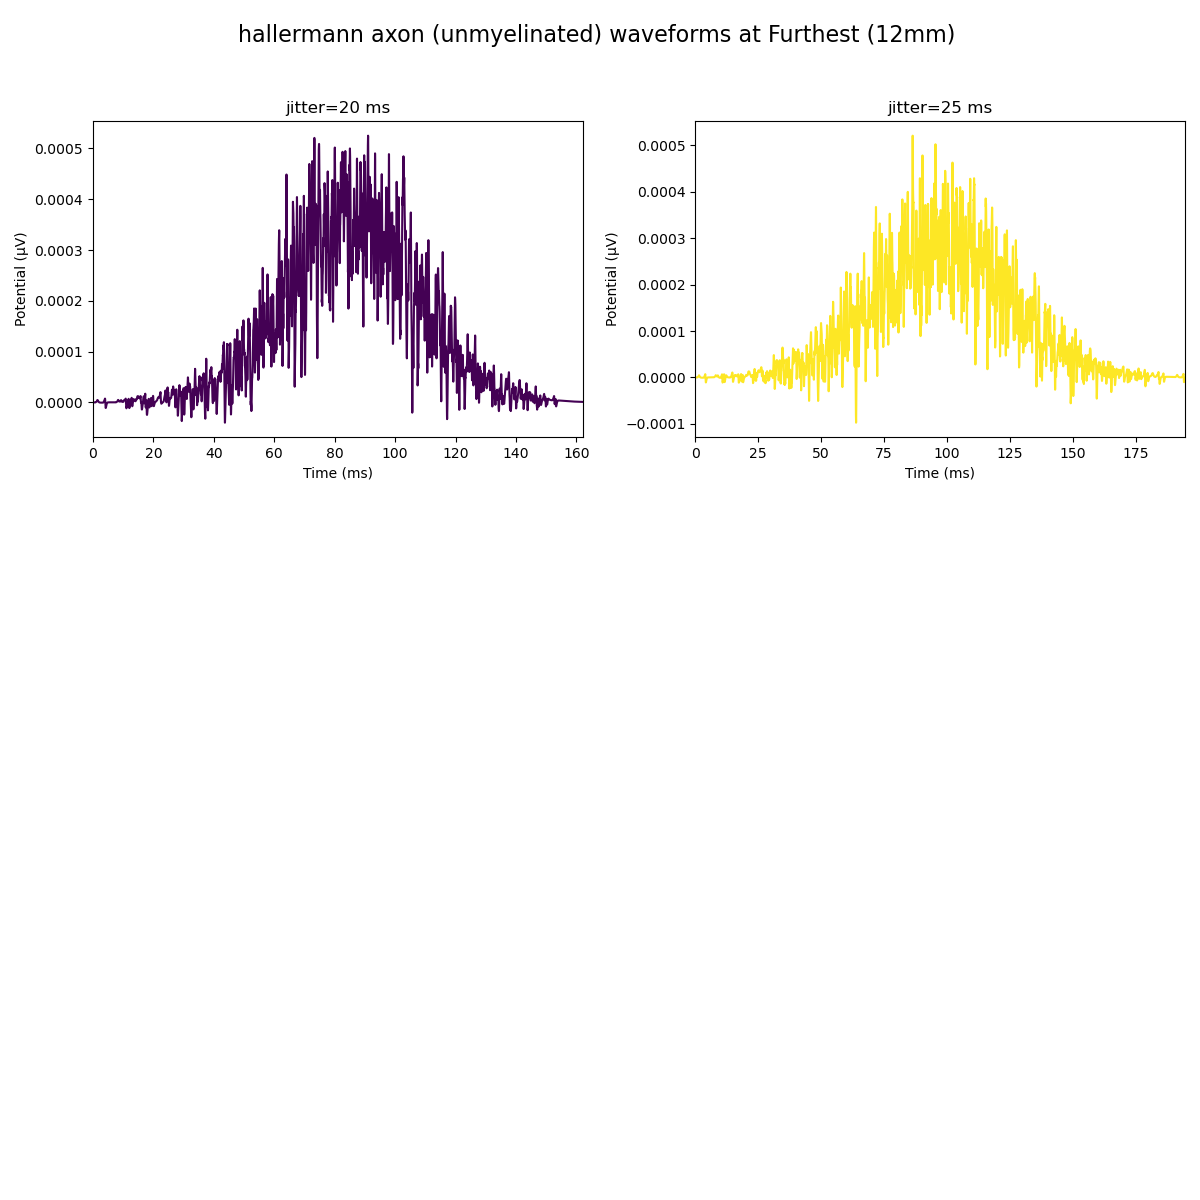
\includegraphics[width=1.2\linewidth]{Figures/axonjitters2EEG.png}}
    \caption{(Continued) Waveforms for the \texttt{hallermann\_axon} cell model without myelination at the furthest electrode (12 mm) with a higher EEG-like conductance and a population size of 10 000 with different jitter.}  
    \label{fig:axonjitters2eeg}
\end{figure}

\newpage
\subsection{Peak Amplitude Analysis}\label{subsec:PeakAmplitude}

The primary objective of this study was to investigate how the peak amplitude of extracellular potentials scales with the number of neurons and their temporal synchrony. The simulations included six cell types: Hallermann axon (myelinated and unmyelinated), and four types of Hay pyramidal cells (active soma, soma, apical, and single apical exp) as detailed in Section \ref{subsec:cellmodels}. For these extracellular potentials, two electrode configurations were chosen: the Closest (10 µm) electrode and the \texttt{RecExtElectrode} High Conductivity electrode as described in Section \ref{subsec:Electrodes}.

\subsubsection{Peak Amplitude vs. Population Size}

Figures \ref{fig:PeakAmpECoG} and \ref{fig:PeakAmpEEG} display the relationship between population size and peak-to-peak amplitude for each cell type across varying jitter levels (0 ms to 25 ms). The x-axis represents the logarithmic scale of population size, while the y-axis, also logarithmic, shows the amplitude in microvolts (µV).

\begin{figure}[p]
    \vspace*{-3cm}
    \centering
    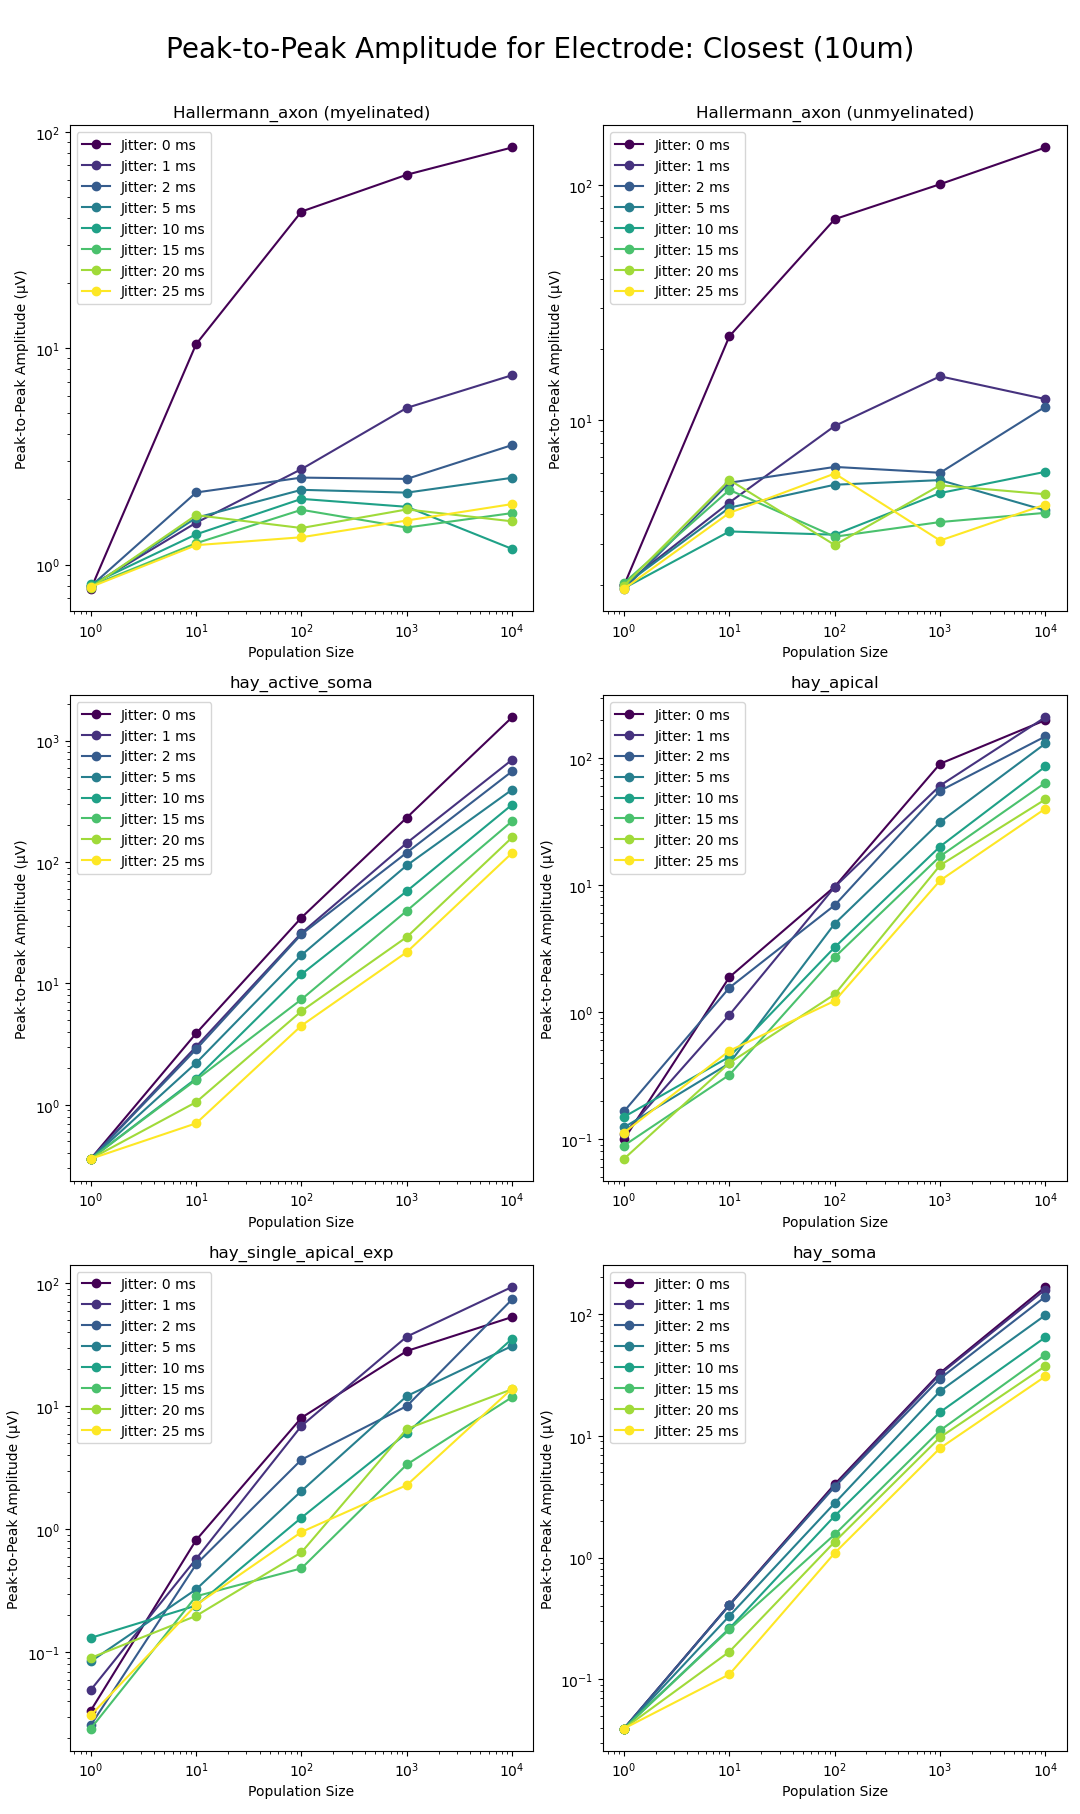
\includegraphics[width=\textwidth]{Figures/PeakAmpECoG.png}
    \caption{Peak amplitude vs. population size recorded using the closest (10 µm) electrode for various cell types and jitter levels. The x-axis represents the population size, while the y-axis shows the peak amplitude in microvolts (µV). Both axes are logarithmic}
    \label{fig:PeakAmpECoG}
\end{figure}

\begin{figure}[p]
    \vspace*{-3cm}
    \centering
    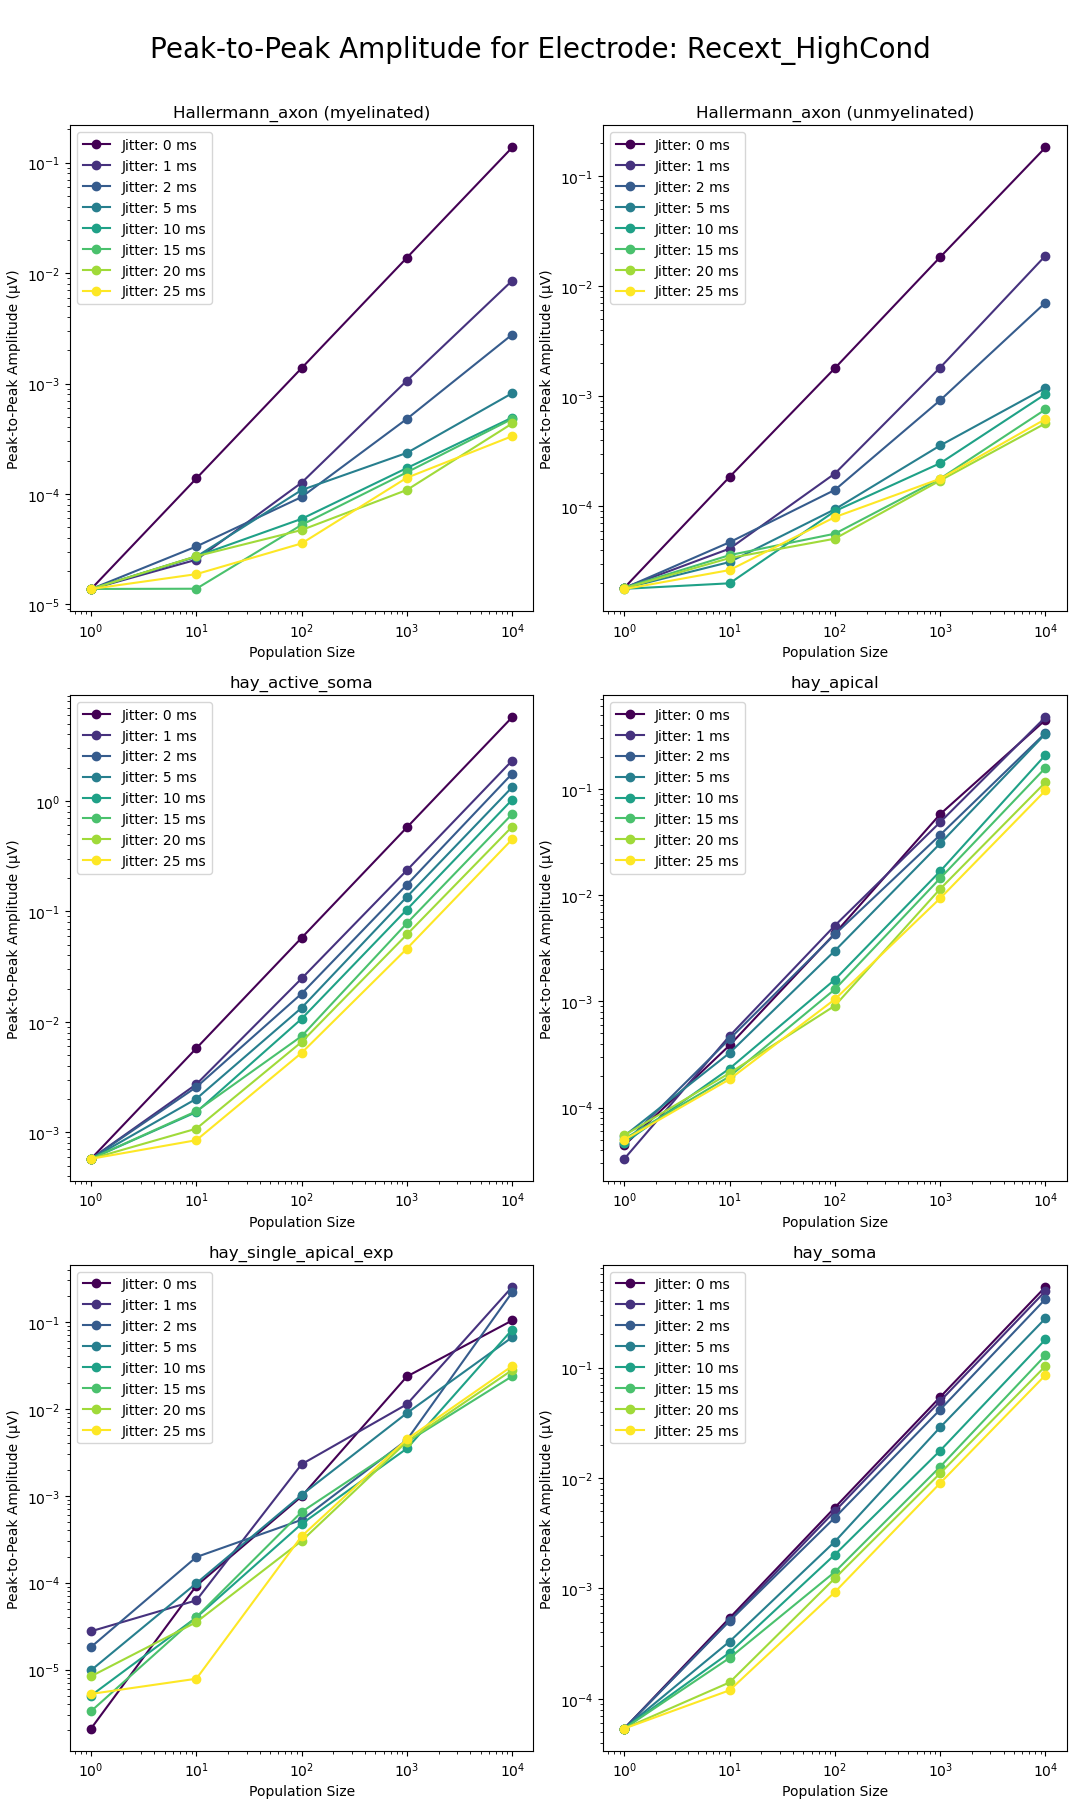
\includegraphics[width=\textwidth]{Figures/PeakAmpEEG.png}
    \caption{Peak amplitude vs. population size recorded using the four sphere approximation electrode for various cell types and jitter levels. The x-axis represents the population size, while the y-axis shows the peak amplitude in microvolts (µV). Both axes are logarithmic}
    \label{fig:PeakAmpEEG}
\end{figure}

\subsubsection{Closest (10 µm) Electrode}

The peak amplitude for the Closest electrode shows distinct patterns between cell types. For Hallermann axon models, the unmyelinated axon exhibits a higher peak amplitude compared to the myelinated variant, especially at low jitter levels. As the population size increases, the peak amplitude generally increases for Hallermann axons, but an increase in jitter gives lower amplitude, indicating a dispersive effect. The amplitude also increases less for each enlargement in population size for the axons. On the other hand, the Hay cell types show a more consistent increase in peak amplitude with population size.

\subsubsection{EEG-like High Conductivity Electrode}

For the \texttt{RecExtElectrode} with higher conductivity, the overall amplitude is significantly lower compared to the Closest electrode, reflecting the attenuation effect of the distance through the head. The pattern of increasing peak amplitude with population size remains consistent across Hay cell types, although the absolute values are lower. The Hallermann axon models still exhibit a decrease in peak amplitude with increasing jitter, but the difference between the myelinated and unmyelinated variants becomes less pronounced compared to the Closest electrode. All populations have linear scaling for synchronized firing. 


\subsubsection{Effects of Axonal Depth} \label{subsubsec:depth}
Figure \ref{fig:AxonDistancesPeakAmpECoG} shows the peak amplitudes of axons simulated with the original simulation code before the changes outlined in Section \ref{subsubsec:CodeChanges}. Here the jittered values show a decrease in signal for almost all jitter values above 0. The non jittered populations had similar scaling as in the newer simulations, but with slightly lower peak amplitudes. 

\begin{figure}[htbp]
    \centering
    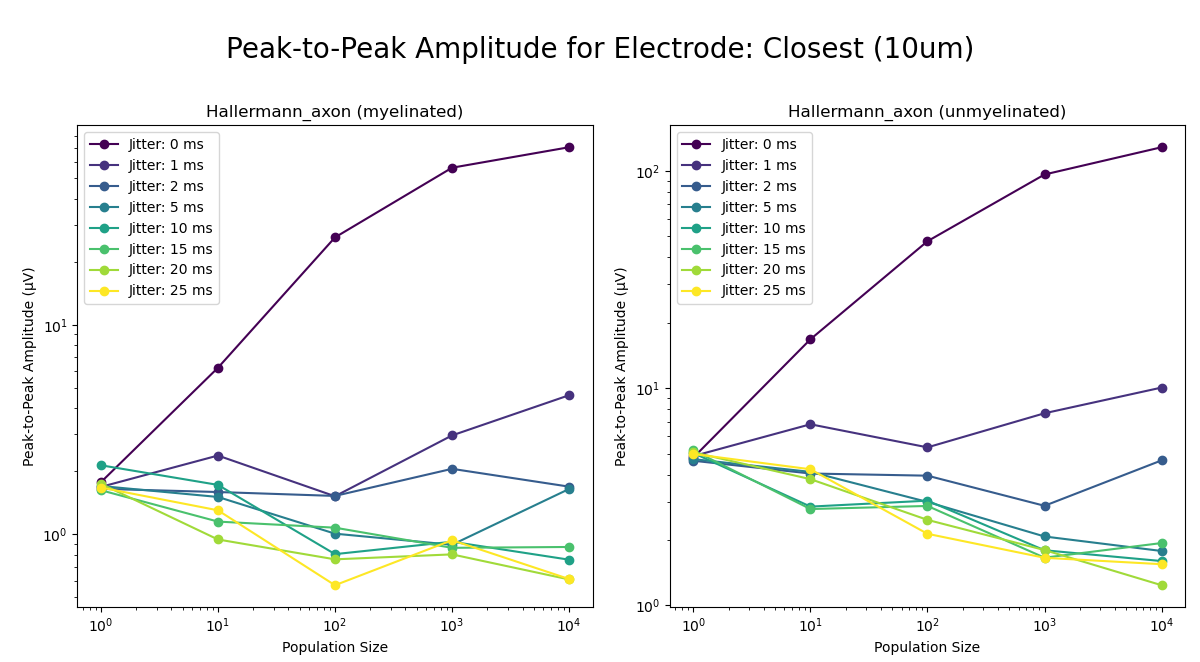
\includegraphics[width=\linewidth]{Figures/AxonDistancesPeakAmpECoG.png}
    \caption{Peak amplitude vs. population size recorded using the closest (10 µm) electrode for the Hallermann axon (both myelinated and unmyelinated) with varying jitter levels. The x-axis represents the population size, while the y-axis shows the peak amplitude in microvolts (µV). Both axes are logarithmic. These measurements were done with the first code meaning the variation of the depths of the axons was larger.}
    \label{fig:AxonDistancesPeakAmpECoG}
\end{figure}

\subsection{Combined Cell Simulations}
Figure \ref{fig:combinedwavecog} and Figure \ref{fig:combinedwaveeg} illustrates the waveforms of populations of 10 000 of combined cells for different jitter values for both an ECoG-like and an EEG-like electrode. These were simulated with unmyelinated input axons and synapses firing 1 ms after the spike hits the top of the axon. In these plots, this single ms of delay was removed later by shifting the potentials from the axons 1 ms later. The axon signal was not scaled compared to the complete cells for these unmyelinated axons. All results from combined models used the unmyelinated axons variant. As is apparent from the waveforms, a synchronized population is essential for the action potential to be visible. The positive spike before the actual action potential is the signal from the electrical stimulation to the axon hillock. 

\begin{figure}[htbp]
    \centering
    \vspace*{-3cm}
    \makebox[\linewidth]{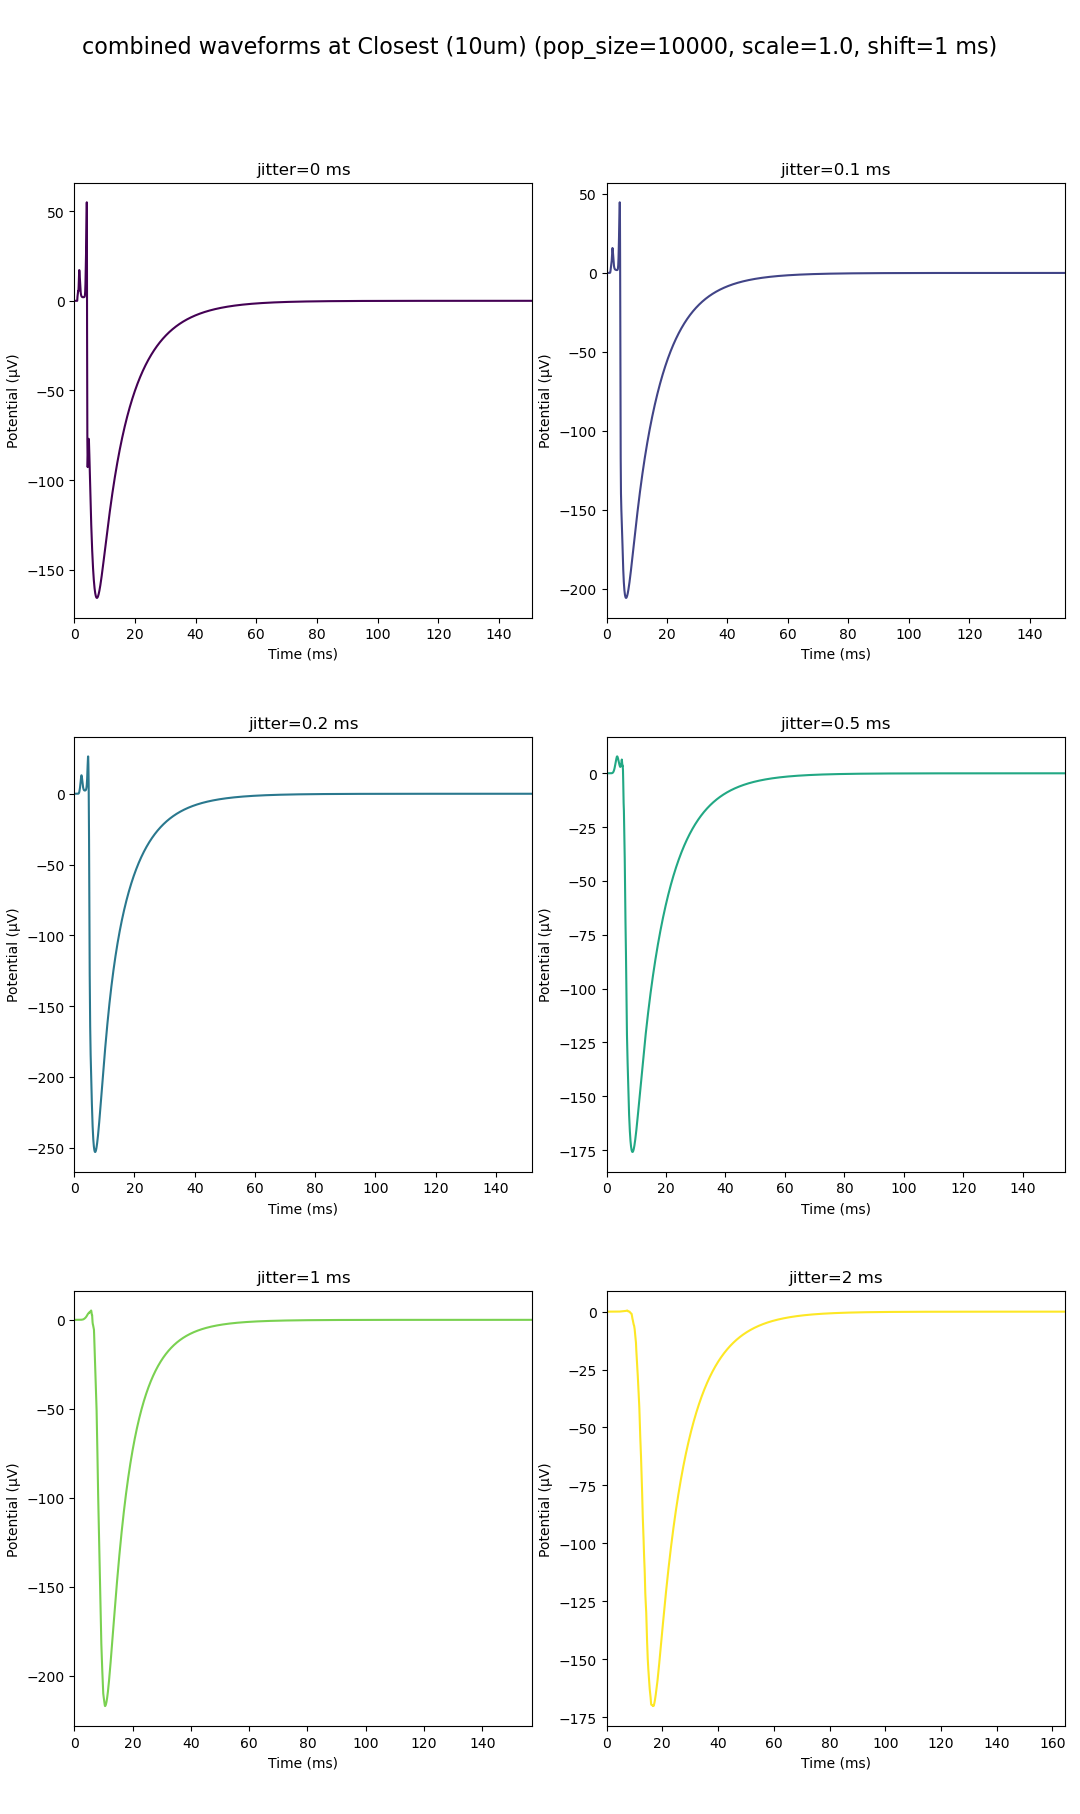
\includegraphics[width=1\linewidth]{Figures/combojitterECoG.png}}
    \caption{Waveforms for the combined cell model at the closest electrode (10 $\mu$m), a population size of 10 000 and varying jitter values.}
    \label{fig:combinedwavecog}
\end{figure}

\begin{figure}[htbp]
    \centering
    \vspace*{-3cm}
    \makebox[\linewidth]{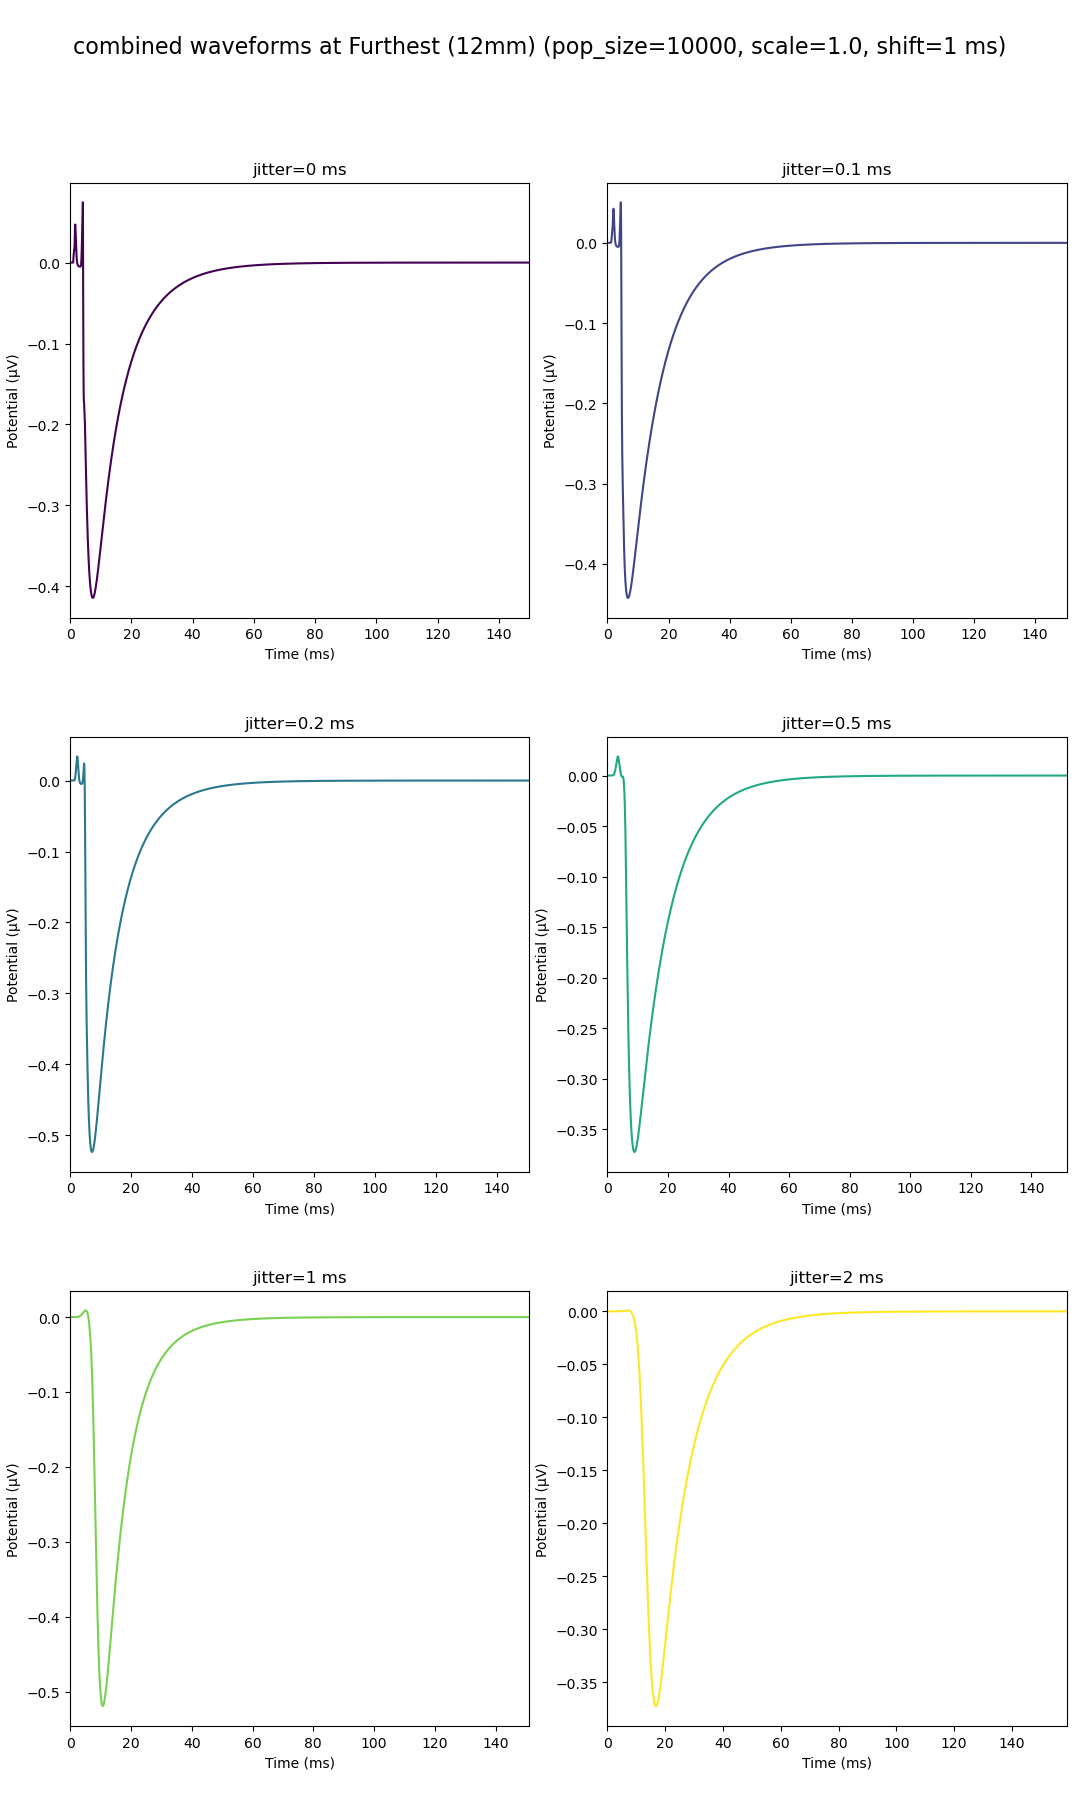
\includegraphics[width=1\linewidth]{Figures/combojitterEEG.png}}
    \caption{Waveforms for the combined cell model at the furthest electrode (12 mm) with higher conductance to be more like actual EEG, a population size of 10 000 and varying jitter values.}
    \label{fig:combinedwaveeg}
\end{figure}

The two sets of waveforms are quite similar. Both exhibit a small spike before the spike from the axons and a large and sustained negative deflection corresponding to the PSP from the cells. The negative deflection is around four times larger in amplitude than the positive deflection for populations with 0 jitter. The signals still exhibit this positive spike before a negative deflection up to and including 1 ms of jitter. After this, the positive spike is gone. The waveforms from the two electrodes are very similar for each jitter value, but the closer field recordings are a bit more "choppy" than the far field recordings. 

\clearpage
\section{Discussion}
\subsection{\texttt{FourSphereVolumeConductor} Approximations}
As can be seen from the results in Figure \ref{fig:FourSphereComp} and Table \ref{tab:FourSphereAmps}, there were quite large differences between the different electrodes used. The electrode with the largest signal was the one assuming the lowest conductance. This might seem counterintuitive, but makes sense when considering the impedance of the electrode-tissue boundary. A lower conductance will lead to a higher impedance, and therefore the signal will be less dissipated in the medium. This discovery prompted the creation of the electrode with a higher apparent conductance, as outlined in Section \ref{subsubsec: find sigma}. This value was a lot better fit, giving the same max potential and almost the same trace as the actual \texttt{FourSphereVolumeConductor} potential. A notable observation is also that the standard extracellular conductivity of 0.3 $S/m$ gave measurements not far from the target, only missing the actual value of the \texttt{FourSphereVolumeConductor} electrode by a factor of \textbf{$\approx$3}. This was opposed to the combined conductance model, which had an error of about 50 times too much power in the signal. Because of this observation the 1 $S/m$ \texttt{RecExtElectrode} was implemented, giving a much better approximation as well as saving a lot of time during the simulations. Each measurement with the \texttt{FourSphereVolumeConductor} took in the neighborhood of 23 seconds per measurement, while the \texttt{RecExtElectrode} took less than a second. Findings in this thesis should still be applicable, as the readings from the improved approximation and the actual four sphere model were so similar.
Note that this value for an approximated electrode has not been verified outside of the scope of this thesis, and as such might only be applicable to the cases simulated here. The approximation held for both complete Hay cells and Hallermann axons, but might break down for other cells or different parameters in other simulations. 

\subsection{Summation of Single Neuron Waveforms}
The essence of measuring brain potentials is summing of small signals to get a larger waveform. Each little neuron contributes and the sum of all the small parts is the resultant signal. This is exemplified in Figures \ref{fig:apicalwav}, \ref{fig:axonwavmyen}, and \ref{fig:axonwavunmyen}. Here the waveforms of single cells are displayed in the first plot. The short spike from the action potential spans only about 1 ms whereas the signal from apical input to the pyramidal cell spans up to 30ms. Another important note when summing these signals is the fact that the AP is both positive and negative, whereas the PSP is (in this case) only negative. This opens the AP up to both constructive and destructive interference while the PSP only experiences constructive interference. This is the main reason for the much larger amplitudes for populations of Hay cells compared to the Hallermann axons.
\newline In real cells the axon can terminate in the apical tuft of the pyramidal cell and activate synapses there. This is also approximated in the combined simulations in this thesis. Here the axons AP spikes up first, then the longer PSP from the pyramidal cell pulls the potential negative for a longer while afterwards. This can also be seen in Figure \ref{fig:combinedwavecog} where a population of 10 000 combined cells was simulated. In this more realistic scenario the AP is clearly visible when the cells are perfectly synchronized, but with just a little bit of jitter the spike vanishes quickly. As can be seen from \ref{fig:combinedwaveeg} this effect is still visible on the EEG-like electrodes as well, albeit with far lower amplitude. When the standard deviation for the jitter is less than or equal to 1 ms the positive spike is still visible. It might not be measurable as the signal ratio falls of dramatically with even 0.1 ms of jitter. For fully synchronized firing the positive spike is about 1/4 the amplitude of the negative deflection. When the jitter increases to 0.1 ms this relation decreases to around 1/5. Already at 0.2 ms the positive spike is 1/10 of the negative deflection and at 0.5 ms the spike is barely visible. This indicates that axons \emph{do} have an impact on measured brain potentials, but only in certain circumstances where the signals are well synchronized. For populations where the axons are not synchronized the potentials from each spike will destructively interfere, reducing the amplitude of the resultant total potential. 

\subsection{Attenuation due to Distance}
The results in Section \ref{subsubsec:depth} compare the peak to peak amplitudes of axons as seen in Figures \ref{fig:PeakAmpECoG} and \ref{fig:AxonDistancesPeakAmpECoG}. Here the amplitudes in Figure \ref{fig:AxonDistancesPeakAmpECoG} show the results before the changes outline in Section \ref{subsubsec:CodeChanges} were made. The amplitudes of jittered axons trend towards destructive interference and for all values above 1 ms of jitter the total signal from populations of any size is \emph{smaller} than the signal of a single axon. This was an unexpected result and prompted the change in the code as described in Section \ref{subsubsec:CodeChanges}. After adjusting the code the results looked better and more like the theory would suggest. These more expected results can be seen in Figure \ref{fig:PeakAmpECoG}. Here the axon populations keep on summing and giving a larger peak amplitude than for single axons. This is more inline with the expected results. The old simulation code had a lot more variance in the depth of the axons and this accounts for the difference between the two results. The fact that this small change in the simulation code had such an impact on the results show that the placement of the axons and the distance from the electrode is crucial for a clear signal. 
\newline This attenuation due to distance is also apparent in Figure \ref{fig:axonmyenelecswav} where all the electrodes are plotted. The distances for each electrode is outlined in Table \ref{tab:elecdist} and for the later electrodes which are placed further from the population the signal is a lot lower than for the closer field electrodes. Compared to the closest few electrodes (10-100 $\mu$m from the populations) the signal from the furthest electrodes (6-12 mm from the population) is almost invisible. 
The effect of distance attenuation is apparent and comparable for all simulations presented in this thesis. All simulations fell about three orders of magnitude when moving from the closest electrode to the furthest. 
\newline As a consequence of this the positive signal from the combined cells gets an amplitude of around 1 $\mu$V for the synchronized populations, as can be seen in Figure \ref{fig:combinedwaveeg}. Usually brain potentials need to be on the order of at least 10 $\mu$V to be measurable and discernible from the noise in the brain. This indicates that 10 000 perfectly synchronized cells are not enough for the AP to be visible in EEG conditions. Still, the positive spike might be visible if even larger populations on the order of 100 000 to 1 000 000 cells fire in unison. 

\subsection{Population and Jitter Effects on Peak Amplitudes}
The simulation results from Section~\ref{subsec:PeakAmplitude} clearly show how both population size and spike-time synchrony affect the peak extracellular signal amplitude, with distinct behaviors at the near-field (intracortical/ECoG-like) versus far-field (EEG-like) electrodes. Figures~\ref{fig:PeakAmpECoG} and~\ref{fig:PeakAmpEEG} illustrate the peak-to-peak voltage recorded as a function of the number of simultaneously active neurons under various spike-time jitter conditions. In broad terms, larger neuron populations produce higher peak signals, but this scaling is strongly modulated by the degree of synchrony in their firing. The contrast between the closest electrode (10~µm from the neurons) and the distant EEG-like electrode is especially striking: near the source, even relatively small synchronous populations can produce substantial voltage deflections, whereas at the far-field electrode, appreciable signals only emerge for very large and highly synchronized populations.

This section examines these trends in detail, comparing the contributions from different neuronal compartments: Isolated axonal spikes (Hallermann axon model, with and without myelination) versus somatic and dendritic synaptic potentials in a pyramidal cell (Hay model) as population size and timing jitter vary. The findings are then related back to the initial hypotheses about axonal versus dendritic contributions to extracellular potentials (see Section~\ref{subsec:AxonalContributions}).

\subsubsection{Near-Field Results (Closest Electrode, 10µm)}
At the nearest electrode, peak amplitude rises markedly with population size, consistent with the expectation that contributions from individual neurons sum when they fire together. In the absence of any spike-timing jitter (0 ms dispersion), this relationship is close to linear: adding more simultaneously active neurons leads to an almost proportional increase in the peak voltage. For example, multiplying the population by 10 from 10 to 100 neurons nearly increases the peak amplitude by an order of magnitude in the 0~ms jitter condition. Most source types follow this trend under perfect synchrony, although their absolute signal magnitudes differ due to the different biophysical properties of axons, somas, and dendrites. For axons the summation for perfect synchrony is less than linear.

Introducing spike-time jitter greatly reduces the efficiency of this summation. Even at the 10µm electrode, a slight desynchronization among neurons causes the peak amplitude to grow sub-linearly with population size. In other words the actual signal is below that of $N * single cell signal$. When a timing jitter of 1 ms is applied the peak amplitude still increases with the number of cells, but not as steeply as in the perfectly synchronous case. The growth curve tapers downward for larger populations. Each additional neuron contributes a bit less to the peak because its spike may not coincide exactly with the others. Quantitatively, the effect is noticeable: for example, at $N=100$ neurons, a 1 ms timing jitter can reduce the peak amplitude to on the order of $80\%$–$90\%$ of the no-jitter value (exact values depend on the cell type). With more severe desynchronization (e.g. 5 ms jitter or more), the peak-amplitude-versus-population curve eventually almost plateaus beyond a certain population size. In other words, beyond some point, adding additional out-of-sync neurons yields little to no further increase in the maximum signal—their contributions are too temporally dispersed to sum constructively. In the extreme case of 25 ms jitter, thousands of neurons firing within a wide time window produce a peak amplitude only on the order of a single neuron’s spike. This highlights that tight temporal coherence is crucial for achieving large peak signals, even locally.

Another factor contributing to the sublinear growth at large population sizes is the spatial distribution of the neurons. In our simulations the neuron density is kept fixed, so a larger population occupies a broader area. Neurons at the periphery of an enlarged population are slightly farther from the electrode than those at the center, so their spikes produce a somewhat smaller signal at that electrode. This geometric effect means that as population size increases, a diminishing fraction of each added neuron’s current contributes maximally to the recorded peak. This effect is especially important for the axons. Here the summation is less than linear from 10 neurons and up. This is most likely due to the increased distance from the axon to the electrode. This makes each new cell's contribution to the total potential decrease. Figure~\ref{fig:PeakAmpECoG} illustrates this phenomenon for the axon-only simulations: even with perfect synchrony, the incremental gain in peak amplitude per added axon diminishes as the cluster’s radius grows, and with jitter the summation is further blunted. 

This is more apparent in Figure \ref{fig:AxonDistancesPeakAmpECoG} were the pre-modification code was used. Here the cells were placed with a lot more variance than in the final simulation code. It seems this effect made more axonal spikes sum destructively and also contribute less to the total signal as a function of their distances to the electrode. The total effect of this seemingly leads to a reduction in signal as long as there is any jitter and a big variance in population height. This solidifies the assumption that axons can contribute meaningfully to measured brain potentials, but only in some circumstances and not always.

Thus, both timing dispersion and spatial dispersion limit the growth of peak amplitude in the near-field configuration. These near-field observations align well with theoretical expectations. In particular, they provide concrete modeling evidence for the idea that local field potentials (and by extension ECoG signals) are strongest when neurons fire in unison, as hypothesized in Section~\ref{sec:theory}.

\subsubsection{Far-Field Results (EEG-like Electrode)}
Recordings at the far-field (scalp) electrode present a markedly different picture. At the EEG-range electrode distance, absolute signal amplitudes are dramatically smaller, and the requirement for synchrony is even more pronounced. That is, the signals are small, but the summation effects actually seem stronger than for near-field recordings. Even with zero jitter, the peak voltage from a given population is orders of magnitude lower than at 10µm. For example, whereas a population of a few hundred perfectly synchronized pyramidal cells might produce a local peak on the order of tens to hundreds of microvolts at the intracortical electrode, the same population yields only a few microvolts at the scalp. This steep attenuation is expected given the distance and the insulating effects of skull and cerebrospinal fluid (see Section \ref{subsec:Electrodes}). More revealing is how differently the various cellular components contribute at this far-field scale. Orientation and spatial alignment of transmembrane currents become critical for constructive summation at the scalp. When many pyramidal cells receive simultaneous apical drive, their combined current dipoles (sinks in the distal dendrites and return sources at the somatic/proximal regions, all aligned normal to the cortical surface) sum coherently. Consequently, on the order of 1000 perfectly synchronized dendritic events can produce a clear far-field signal on the order of a few microvolts. In contrast, populations of pure axonal spikes are far less effective at driving scalp potentials: even a very large population (e.g. 1000 axons firing together) generates on the order of only $10^{-2}$µV (tens of nanovolts) at the scalp. Myelinated axons produce slightly lower EEG peaks than myelinated axons in these simulations, but both axonal cases remain one to two orders of magnitude smaller than the dendritic contribution. 
As in the near-field case, spike-time jitter diminishes far-field peak amplitudes, but the impact of desynchronization in the axons is less severe when taking relative signal levels into account. This indicates that the synchronization is not as important for far-field recordings, but will still lead to higher signals than unsynchronized neurons. Jittering is also less important for the other models showing close to linear scaling in all cases. These results underscore that under realistic conditions, axonal action potentials contribute minimally to EEG signals, whereas synchronized dendritic currents in aligned neurons can generate significant deflections. Another interesting observation is the fact that axonal potentials fell three to four orders of magnitude when moving from near-field to far-field. In comparison, the other models all fell a bit less, indicating that the spatial attenuation effects are a bit less severe for synaptic potentials than action potentials. The relatively large variance observed in the \texttt{hay\_single\_apical\_exp} case is likely due to the random placement of the single synaptic input, meaning the actual distance from the electrode varies between trials.

\subsubsection{Implications and Alignment with Initial Hypotheses}
These findings strongly support our theoretical framework (see Section~\ref{subsec:AxonalContributions}) that dendritic currents in aligned pyramidal cells are the primary contributors to ECoG and especially EEG signals, whereas the contribution of axonal action potentials is minimal. Even under highly favorable conditions, thousands of neurons firing together, my models show that peak scalp voltages from synchronous axonal spikes remain one to two orders of magnitude smaller than those from synchronous dendritic events. This reinforces the classic interpretation that typical EEG/ECoG peaks predominantly reflect summed postsynaptic (dendritic) potentials rather than axonal spikes.

In spite of this, the results also show that for closer field recordings axonal activity is more important. This is especially true for synchronized firing, where the axon signals has been shown to match or even surpass signals from PSPs. It is also apparent that the summation effects of the axonal activity is stronger at the EEG-like electrode for more realistic jittering values. Still, the potentials seen are under the noise floor of most modern EEG recorders and as such will most likely not be visible on recordings as the noise from other electrical signals and the amplification itself can mask the signal.

Moreover, the observed plateauing of the peak amplitude with increasing jitter quantitatively defines the limits of temporal summation discussed in Section~\ref{subsec:populationMethod}. Beyond a few milliseconds of spike-time dispersion adding more axons does not substantially increase the peak signal because the lack of simultaneity prevents their contributions from aligning. The slight sublinear scaling with very large populations in the near-field similarly echoes our spatial summation considerations: as neuron clusters grow, their signals do not add perfectly due to the increasing source–electrode distance for cells at the periphery. Overall, these results illustrate how population size, synchrony, spatial scale, and neuron morphology jointly determine the relationship between microscopic neural events and the macroscopic potentials they generate. The convergence of these simulation outcomes with our initial hypotheses provides confidence in the modeling approach and offers a quantitative basis for understanding and extrapolating to more complex brain activity patterns.

\subsection{Limitations of This Thesis}
The simulations in this thesis do, to a certain degree, use arbitrary values for a lot of parameters that might not be entirely analogous to real conditions in the brain and might therefore not be directly applicable to real world measured brain potentials. For instance, the chosen values for synaptic weight and timing might not be realistic in comparison to  the strengths of spikes from the axons. The creation of populations also has some limitations because, when only a single cell is used, it is placed at the bottom center of the population cylinder. Therefore, the effective distance for a single cell to the electrode is whatever height the electrode has + the max height of the population. When creating larger populations the cells are uniformly distributed from the first cell and upwards toward the "roof" of the population cylinder, meaning these come closer to the electrode and as such will contribute more to the potentials. This might influence the signals measured, especially close to the neural sources. Keeping the height of the populations static also changes the width of each population by a lot which can have a substantial effect on the measured brain potentials, in particular for near-field measurements. The EEG-like electrodes which are placed further away are less susceptible to this variance in both cell placement and population size as the variance in distance is negligible compared to the distance from population to electrode. Nevertheless, results and conclusions found during simulations of brain activity might give an indication as to what might be possible to observe in vivo and should therefore serve as inspiration for both further discussion and research into the contribution of axons to measured brain potentials. 
\newline
The cells used in these simulations are both based on cells from the rat cortex. Cell densities are taken from estimates on the density of the mouse cortex. While mammalian cortices are similar to a degree, they might not be perfectly analogous. At the same time, these models are time tested and have been utilized for many scientific publications earlier and as such findings from these simulations are still valuable.
\newline
The populations simulated were also quite small due to the computational cost of running simulations. The radius for the largest populations simulated were still only about 1 mm and as such would encompass a very small region of the brain. A bigger population of 100 000 cells would have a radius around 3.5 mm and therefore be closer to real recording areas of electrodes which usually span a couple of millimeters in diameter for ECoG and up to a centimeter for EEG. This would make for more realistic simulations of ECoG signals. A population of 1 000 000 neurons might give more accurate EEG signals as well. This would, however, take on the order of 3 days to simulate for one jitter value and cell type and as such was not possible for this thesis with its current methods. The computational cost of these simulations became apparent early, and the simulations were evidently single core CPU bound, but a solution to this was not found. As a brute force approach to speed up simulations multiple lightweight virtual machines were utilized simulating different models in order to have simulations running in parallel. 
\newline
The simulation of combined cells is not especially accurate to real cells. The axon and cell have a somewhat random placement, which could be improved. As is, the axon and cell are placed in the same spot, meaning the soma of the cell is below the hillock of the incoming axon. For real cells, the end of the axon will connect to the apical dendrites and, therefore, will dictate the position of the synapses, which was not taken into account here. The axon itself might also be offset or rotated, as compared to how they were simulated in this thesis. All of these considerations will change the resultant waveform, but these results still indicate that measured brain potentials from axons might be worth exploring further.
Additionally, the simulations do not include variability in axonal orientations, lengths, and conduction velocities, factors which could significantly impact the summation of extracellular potentials and the degree of synchronization achieved. Furthermore, simplified head geometry and homogeneous conductivity parameters were used, potentially underestimating real-world attenuation and spatial filtering effects, thus limiting the precise quantitative applicability of these results to in vivo conditions.
\newline
The effects of randomness on the measured potentials was not mitigated in any way. All simulations were ran only once and were not cross-checked with different seeds or using other techniques to average out the effects of the inherent randomness in the simulations. To make more robust conclusions, each simulation should be attempted more than once and then the results averaged. This would remove at least some outliers, as was apparent in the \texttt{hay\_single\_apical\_exp} results. Here a random location for an apical synapse was chosen, and this lead to a lot of variation in the peak amplitude of the potentials, even for a single cell. A more deterministic simulation could also be an option, but the parameters would need to be closer to real values.
\newline
Because of the electrical stimulation for the axons there are some artifacts in their waveform. This is apparent in all results where axons are involved and as such affects both axons and the combined cell models. This early spike from the electrical stimulation can be clearly seen in Figure \ref{fig:axonmyenelecswav} where there are two positive spikes before the negative part of the action potential. The first spike is the electrical stimulation and the second is the actual action potential. This artifact will likely lead to a bit higher signals than what is realistic. As such, a better approach would be to remove this stimulation deflection before summing the signals. This was not done for this thesis and therefore the axon waveforms and combined waveforms might be a bit more positive than they would be in reality.

\subsection{Outlook}
Future work should aim to refine computational models by incorporating more biologically realistic axonal geometries and precise synaptic placements to enhance simulation accuracy. Experimental validation of axonal contributions in highly synchronized states through in vivo studies or controlled in vitro setups could further substantiate the simulation findings. Additionally, exploring pathological brain states characterized by increased synchronization, such as epilepsy, might provide deeper insights into conditions under which axonal contributions become prominent. It would also be valuable to investigate how varying degrees of synchrony influence the detectability of axonal signals, potentially redefining conventional EEG/ECoG modeling approaches. Furthermore, advancements in measurement technology, which lowers the noise-floor in amplifiers, might enable more accurate reading of these axonal contributions. As such, this discussion might be at a stand still until more advanced measuring equipment is developed to be able to measure these potentials in vivo. Future experimental work could specifically aim to validate the contributions identified in simulations by employing pharmacological manipulations, such as the selective inhibition of axonal spikes, to differentiate clearly between axonal and synaptic sources of measured potentials. Additionally, incorporating axonal conduction delays and variability in axon morphology into computational models would enhance the understanding of their impacts on measurable brain potentials and clarify under which conditions these axonal signals become reliably detectable.

\subsection{Conclusion}
This thesis investigated the contribution of axonal action potentials to measured brain potentials, using computational models simulating EEG and ECoG recordings. The results demonstrated that while traditionally axonal contributions are neglected due to presumed cancellation effects, axons can influence recorded potentials under conditions of high neuronal synchrony. Although minimal in far-field EEG measurements under typical conditions, axonal potentials can become comparable to dendritic contributions at closer, intracortical distances when firing synchrony is high. Thus, axonal currents, traditionally overlooked, are important components in accurate ECoG signal modeling, but also for EEG signals, particularly under synchronized neuronal activity conditions where the resultant signals might be above the noise floor of the amplifiers. These findings challenge established assumptions, and strengthen modern theories emphasizing the importance of including axonal contributions in neural field models for certain physiological and pathological states. The findings presented explicitly challenge traditional modeling assumptions by demonstrating scenarios where axonal contributions become non-negligible, thereby highlighting the need to reconsider the interpretation of EEG/ECoG signals, especially under conditions characterized by significant neuronal synchronization such as epileptic seizures or evoked brain responses.

\clearpage
\references
\clearpage
\appendices 
\section{Simulation code}\label{app:simcode}
\inputminted[linenos]{python}{Appendicies/Simulation.py}
\end{document}

